\documentclass[a4paper,11pt]{report}

\usepackage{parskip}
\usepackage[margin=2.54cm]{geometry}
\usepackage[utf8]{inputenc}
\usepackage{graphicx}
\usepackage[table,xcdraw]{xcolor} 
\usepackage{pdfpages}  %to insert pdf documents
\usepackage[draft]{todonotes}
\usepackage{pdflscape}
\usepackage{teresa}  % this is the project-layout style

%Joao Imports
\usepackage{framed,color}
\definecolor{shadecolor}{rgb}{0.9,0.9,0.9}
\usepackage[hidelinks]{hyperref}
\usepackage[hyphenbreaks]{breakurl}
\usepackage{multirow}
\usepackage{subcaption}
\usepackage{amsfonts}
\usepackage{amsmath}
\usepackage{amsthm}
\usepackage{amssymb}
\usepackage{tikz}
\usetikzlibrary{patterns}
\usetikzlibrary{shapes.geometric}
\usetikzlibrary{calc}
\usetikzlibrary{shapes,arrows,chains}
\DeclareMathOperator*{\argmin}{\arg\!\min} 
\DeclareMathOperator*{\argmax}{\arg\!\max}
\usepackage{mathtools}
\usepackage{algorithm}
\usepackage{algorithmic}
\renewcommand{\rmdefault}{phv} % Arial
\renewcommand{\sfdefault}{phv} % Arial
 \usepackage[T1]{fontenc}

\graphicspath{{./}{figures/}}
%\theoremstyle{remark}
\newtheorem{req}{Requirement}
%\newcommand{\citn}{\begin{footnotesize}[cit. needed]\end{footnotesize}}
%\newcommand{\sw}[1]{\textcolor{red}{SW: #1}}
%\newcommand{\jtodo}[1]{\todo[inline]{TODO (Joao): #1}}
\newcommand{\halfrule}{\begin{center}{\rule{0.5\textwidth}{.4pt}}\end{center}}
\newenvironment{draftpts}
{\noindent\ignorespaces\begin{shaded}\begin{center}\footnotesize{DRAFT | Topics to include:}\end{center}\begin{small}}
{\end{small}\end{shaded}\par\noindent\ignorespacesafterend}

\setcounter{secnumdepth}{5}
\setcounter{tocdepth}{5}

%% Adapt the version and code to your deliverable.
%% Those values will appear in the header
\delivcode{D5.3}
\title{Feedback Part 2\\ Integrated Feedback System}
%% Running title
\titlefoot{Feedback Part 2 -- Integrated Feedback System}

\duedate{M30 -  May  31, 2016}
\wpleader{UvA}
\security{Public} %Public or private
\status{Submitted} %Submitted
\delivversion{1.0}



\begin{document}

\maketitle
\makeheader


%%Add a new row with the current version info. 
\begin{documentinfo}

\begin{tabular}{|p{5cm}|p{4cm}|p{5cm}|}
        \hline
        \rowcolor{gray!50}
        Date and Version Number & Author & Comments\\ \hline
        31.05.2016 v1.0 & Jo\~ao Messias \&\hfill Kyriacos Shiarlis & Initial Verson.\\ \hline
\end{tabular}

\end{documentinfo}


\pagebreak
\pagebreak

\tableofcontents

\pagebreak

\listoffigures

\pagebreak

\listoftables

\pagebreak

%\begin{abstract}

%\end{abstract}


\section{Executive Summary}\label{sec:sum}

The TERESA project aims to develop methods that allow a robot to interact effectively with a dynamic social environment. Specifically, we aim to place a semi-autonomous telepresence robot in a day-care center, to allow accessible and seamless communication between its members and remote visitors such as friends and family.\\

 A significant aspect of the project is that cost functions directly related to the movement and behaviour of the robot such as navigation and body pose are partly learned from data instead of being hard-coded. To make this possible, a variety of resources is required such as perception modules, learning algorithms, and of course the data themselves. \\

This deliverable describes the latest advancements 
elements for the TERESA robot through human feedback, in compliance with the 
Description of Work. It discusses:

\begin{itemize}
  \item Learning Algorithms. These are the methods that allow us to associate data from different sensors with feedback from the experiment subjects, into a cost function. We describe the algorithms used and methods for choosing between different design decisions within each algorithm.
  \item Experimentation. We perform experiments with manually 
controlled robots in which the involved subject thinks are autonomous. We describe 
specific instances of such a method, both for social navigation and social conversation scenario, where a 
  large amount of data and human feedback is collected and processed.
  \item Implementation. Using our methods, the collected data and existing algorithms we perform learning in real and simulated robot settings.
\end{itemize}

We present results and progress for all the above topics and explain in what 
ways their respective performance can be improved in the future.

\section{Contributors}\label{sec:cont}

The main contributors to this document are Kyriacos Shiarlis (UvA), Richard Pronk (UvA), Jo\~{a}o Messias (UvA) and Shimon Whiteson (UOXF). The document was reviewed by Luis Merino and Jes\'{u}s Capit\'{a}n (UPO).

\newpage

\section{Introduction}\label{sec:intro}

The technical goal of TERESA is to develop technology that enables a semi-autonomous robot to behave in an acceptable way in social situations. However, it is very hard to determine explicitly what constitutes an “acceptable way” for a robot to behave. Furthermore, imperfections and noise in the sensing and perception systems of the robot might add to the difficutly of designing a social robot. The goal of Work Package 5 is to produce work that overcomes these difficulties and deliver practical methods for improving the social behaviour of the system in a robust manner. This deliverable presents out latest work on learning social policies and cost functions from human interaction. Furthermore it describes both practical and theoretical innovations in the way these cost functions can be integrated.

Firstly in Section \ref{sec:rrt-iros} we present our latest work on Inverse Reinforcement Learning(IRL) for robotic path planning. In the previous deliverable we presented a new method, Rapidly Exploring Learning Trees, which allows learning of Rapidly Exploring Random Trees, from human demonstrations. I this deliverable we present an extension of the method that takes into account the kinodynamic constraints of the robot and we deploy the method on real data collected using the TERESA robot. 

Section \ref{sec:sl_policy} outlines a method that uses data of human demonstrations coupled with Deep Neural Networks, that allows the robot to learn body pose policies. Such policies determine for example how the robot should possition itself in the presence of an interaction target and an interaction group as well as how it should react to their movement.

Next in Section \ref{sec:sl+rl} we demonstrate how the cost functions learned using human feedback in Deliverable 5.3, can be integrated with the system detailed in Section ??. This is done using a novel hierarchical Neural Network architectures that Reinforcement Learning and Supervised Learning simultaneously. We further present an evaluation that shows that the robot can learn to replicate the demonstrated behaviour while at the same time perform well with respect to the given cost function.  

Finally in Section ??, we describe a more theoretical approach to cost function integration. This is based on...MOPOMDP...

\pagebreak


\section{Learning navigation cost functions from demosntration}
\label{sec:rrt-iros}

<<<<<<< HEAD
In the previous deliverable D5.3, we proposed a new Inverse Reinforcement Learning method that allowed us to learn RRT* cost function from demonstrations. We named this method Rapidly Exploring Random Trees and we showed its effectiveness in navigation settings. In this section we report our progress in that direction. Firstly we review our background and method sections from the previous deliverable. We then go on to perform more thorough experiments in order to compare $RLT^*$ with the baseline method of maximum margin planning (MMP). Furthermore we show that our method can be effectively used to deal with kinodynamic constraints that a robot might have and we demonstrate that our method is much faster than simply using a naive implementation. Finally we apply the method to real data collected during the TERESA project in order to derive a cost function for navigation.



\subsection{Approximate Maximum Margin Planning \label{subsec:ammp}}

Section \ref{subsec:inverse_problem} shows how the multiple constraints of \eqref{eq:const1} can be reduced to the single constraint of \eqref{eq:const} for each demonstration. However, this reduction requires an optimal planner to perform the minimisation in \eqref{eq:const1}, which is impractical in many robot applications. Suppose instead that, as in RRT$^*$, we have a mechanism for sampling different paths from $Z_{o,g}$ along with their respective costs and that, for a given finite time budget $T$, this path sampler samples a subset $\tilde{Z}_{o,g} \subset Z_{o,g}$,  Then, we can modify \eqref{eq:const} to demand that our cost function satisfies,
\begin{equation}
	C(\zeta^i_{o_i,g_i}) \leq \min_{\zeta_{o_i,g_i} \in \tilde{Z}_{o_i,g_i}} C(\zeta) \quad \forall i. \label{eq:const_rrt}
\end{equation}
	As $T$ increases, lower cost paths are sampled, making this inequality harder to satisfy. Assuming $\tilde{Z}_{o_i,g_i}$ is constant, we can rewrite \eqref{eq:unconstrained} as:

	\begin{equation} \frac{1}{2}||\mathbf{w}||^2 + \frac{\lambda}{D} \sum_i \big( C(\zeta^i_{o_i,g_i}) - \min_{\zeta \in \tilde{Z}_{o_i,g_i}}\big(C(\zeta) + L_i(\zeta)\big) \big). \label{eq:unconstrained_rrt}
	\end{equation}
This gives rise to an approach we call Approximate Maximum Margin Planning (AMMP). It is similar  to MMP with the crucial difference that the planning step is executed by a sample-based planner and not a deterministic one, like A$^*$. An important consequence is that $\tilde{Z}_{o_i,g_i}$ changes every time we invoke the sample-based planner. Thus, AMMP can be thought of as sampling the \emph{constraints} that we want our cost function to satisfy. The main advantage of AMMP is that it is not bound by the restrictive assumptions of  A$^*$, such as a discrete state-action space and no motion constraints. 

However, an ineffective sampler could yield poor gradient estimates and thus poor solutions. In fact, Ratliff et al.\ \cite{ratliff2009chomp} argue that, for this reason, sample-based planners like RRT are not suited to learning cost functions from demonstration, as the paths sampled by RRT are heavily biased during the sampling process and thus highly suboptimal. However, asymptotically optimal sample-based planners like RRT$^*$ are better able to plan low-cost paths \cite{karaman2011sampling} and thus well suited for use within AMMP.

\subsubsection{Rapidly Exploring Learning Trees \label{subsec:cached}}

As suggested above, a simple way implement AMMP is to use RRT$^*$ as the sample-based planner.  RRT$^*$ can sample low-cost paths, allowing AMMP to learn a good cost function. Furthermore, RRT$^*$ can cope with large and continuous state-action spaces with motion constraints. However, the result is a computationally expensive algorithm that calls the planner $I\times|D|$ times over $I$ iterations, given a dataset of size $|D|$. Furthermore, sampling a separate set of points at every iteration could produce noisy gradients that negatively affect convergence. In this section, we propose Rapidly Exploring Learning Trees (RLT$^*$), which implements AMMP with an RRT$^*$ planner using a novel caching scheme to ensure both computational efficiency and more consistent gradients.

A key observation is that, in RRT$^*$, only the rewiring step depends on the cost function.  The sampling step is independent of it and, especially when motion constraints are present, contains the most computationally expensive operations. These are: 1) fitting and querying a data structure to find the nearest neighbour and the radius neighbours to a newly sampled point, 2) applying the steer function to all neighbours to and from the newly sampled point, and 3) checking for obstacles in these paths. By contrast,  the only potentially expensive operation in the rewiring step is querying the cost of an edge. 

Therefore, a key idea behind RLT$^*$ is to perform the sampling step just once for each data point and cache it for reuse throughout learning. Then, at each iteration, only the rewiring step needs to be repeated as the cost function changes.

Algorithm \ref{alg:rrt_cache} describes the caching step, which takes as input $p$, the number of points to randomly sample from free space; $s_{init}$, the initial point; and $\eta$, the steer step size. For each randomly sampled point $s_{rand}$, we find the nearest neighbour, $s_{nearest}$, from the set of points in the vertex set $V$. We then create a new configuration point $s_{new}$ by steering from $s_{nearest}$ to $s_{rand}$. Next, we query the radius neighbours, $S_{near}$, of $s_{new}$ at a radius determined by  $\min\{\gamma_{RRT^*}(\frac{\log(|V|)}{|V|})^{\frac{1}{d}},\eta\}$. Here, $d$ is the dimensionality of $S$, and $\gamma_{RRT^*}$ is a constant based on the volume of free space (see \cite{karaman2011sampling}).  Next, we determine which points in $S_{near}$ can safely reach $s_{new}$ through the chosen \texttt{Steer} function (lines 13-17). These forward paths are stored in $Paths_{fwd}$. We then perform the same procedure but this time checking the paths from $s_{new}$ to $S_{near}$ and store them in the set $Paths_{bwd}$ (lines 18-22). This algorithm turns the sampling process of RRT$^*$  into a preprocessing step. Consequently, the expensive \texttt{Nearest}, \texttt{Near}, \texttt{Steer} and \texttt{Safe} procedures only need to be repeated $|D|$ times instead of $I\times|D|$ times.


	\begin{algorithm}
	 \algsetup{linenosize=\tiny}
 	\scriptsize
	\caption{\small \texttt{cacheRRT}($n$,$s_{init}$,$\eta$)}
	\label{alg:rrt_cache}
	\begin{algorithmic}[1]
	\STATE $P \gets \emptyset$ \hfill \COMMENT{Initialise the point cache}
	\STATE $V \gets {s_{init}}$
	\FOR{$i=0 \dots n $}
	\STATE $s_{rand} \gets SampleFree_i$
	\STATE $s_{nearest} \gets \texttt{Nearest}(V,s_{rand})$
	\STATE $s_{new} \gets \texttt{Get}(s_{nearest},s_{rand})$
	\STATE $S_{near} \gets \texttt{Near}(V,{s_{new}},\min\{\gamma_{RRT^*}(\frac{\log(|V|)}{|V|})^{\frac{1}{d}},\eta\})$
	\STATE $Paths_{fwd} \gets \emptyset$
	\STATE $Paths_{bwd} \gets \emptyset$
	\STATE $S_{fwd} \gets \emptyset$
	\STATE $S_{bwd} \gets \emptyset$
	\FOR{$s_{near} \dots S_{near}$}
	\STATE $path_{fwd} = \texttt{Steer}(s_{near},s_{new})$
	\IF{$\texttt{Safe}(path_{fwd})$}
	\STATE $Paths_{fwd} \gets Paths_{fwd} \cup path_{fwd}$
	\STATE $S_{fwd} \gets S_{fwd} \cup s_{near}$
	\ENDIF
	\STATE $path_{bwd} = \texttt{Steer}(s_{new},s_{near})$
	\IF{$\texttt{Safe}(path_{bwd})$}
	\STATE $Paths_{bwd} \gets Paths_{bwd} \cup path_{bwd}$
	\STATE $S_{bwd} \gets S_{bwd} \cup s_{near}$
	\ENDIF
	\ENDFOR
	\STATE $V\gets V \cup s_{new}$
	\STATE $P \gets P \cup \{s_{nearest},s_{new},S_{fwd},S_{bwd},Paths_{fwd},Paths_{bwd}\}$
	\ENDFOR
	\RETURN $P$
	\end{algorithmic}

	\end{algorithm}


The output of Algorithm \ref{alg:rrt_cache} is input to Algorithm \ref{alg:plan_cached}, which resembles the rewiring procedure in RRT$^*$ \cite{karaman2011sampling} and returns a low-cost path to the goal. However, unlike RRT$^*$ rewiring, the vertices of the tree and their neighbours at each iteration are already known and contained within the point cache. This speeds computation while keeping consistency between the planners used during learning and final execution. As learning proceeds and the cost function changes, so does the wiring of this tree; however, the points involved do not change. %Note that, despite caching, Algorithms \ref{alg:rrt_cache} and \ref{alg:plan_cached} are consistent with the planning procedure of the RRT$^*$. Consequently, there is no discrepancy between the planner used during learning and execution.

Algorithm \ref{alg:ammp} describes Rapidly Exploring Learning Trees (RLT$^*$), which uses Algorithms \ref{alg:rrt_cache} and \ref{alg:plan_cached}. First, we initialise the weights, either randomly or using a cost function that simply favours shortest paths. Then, for each datapoint $\zeta_i$, we calculate feature sums and run \texttt{cacheRRT}. The main learning loop involves cycling through all data points and finding the best path under a loss-augmented cost function. The feature sums of this path are calculated and subsequently the difference with the demonstrated feature sums is computed. At the end of each iteration, an average gradient is calculated and the cost function is updated. At convergence, the learned weights are returned.

In addition to saving computation time, the use of caching encourages consistency between the gradients computed in each iteration, as they are estimated from the same sampled points.  The effect on the gradients, which resembles that of momentum \cite{polyak1964some}, can improve performance, as our results in the next section show.

	\begin{algorithm}
	\algsetup{linenosize=\tiny}
 	\scriptsize
	\caption{\texttt{planCachedRRT$^*$}($P$,$s_{init}$,$c()$)}
	 \label{alg:plan_cached}
	\begin{algorithmic}[1]
	\STATE $E \gets \emptyset$
	\STATE $V \gets {s_{init}}$
	\FOR{$i=0 \dots |P| $}
	\STATE $(s_{nearest},s_{new}) \gets P_i$
	\STATE $(S_{fwd},S_{bwd}) \gets P_i$
	\STATE $(Paths_{bwd},Paths_{fwd}) \gets P_i$
	\STATE $V\gets V \cup s_{new}$
	\STATE $s_{min}\gets s_{nearest}$
	\STATE $c_{min}\gets \texttt{Cost}(s_{nearest}) + c(path_{s_{nearest},s_{new}})$
	%\FOR{$s_{fwd} \in S_{fwd} $}
	\FOR{$j=0 \dots |S_{fwd}| $}
	\STATE $s_{fwd} = S^j_{fwd}$
	\STATE $path_{fwd} = Paths^j_{fwd}$  
	\STATE $C_{near} \gets \texttt{Cost}(s_{fwd}) + c(path_{fwd})$
	\IF { $C_{near}<c_{new}$}
	\STATE $s_{min} \gets s_{fwd}; c_{min}\gets c_{near}$
	\ENDIF
	\ENDFOR
	\STATE $E \gets E \cup \{(s_{min},s_{new})\} $
	%\FOR{$s_{bwd} \in S_{bwd} $}
	\FOR{$j=0 \dots |S_{bwd}| $}
	\STATE $s_{bwd} = S^j_{bwd}$
	\STATE $path_{bwd} = Paths^j_{bwd}$
	\STATE $C_{new} \gets \texttt{Cost}(s_{new}) + c(path_{bwd})$
	\IF {$C_{new}<\texttt{Cost}(s_{near})$}
	\STATE $s_{parent} \gets \texttt{Parent}(s_{bwd})$
	\STATE $E \gets E  \smallsetminus {(s_{parent},s_{bwd})} \cup {(s_{new},s_{bwd})} $
	\ENDIF
	\ENDFOR
	\ENDFOR
	\STATE $\zeta_{min} \gets \texttt{minCostPath}(V,E,c())$
	\RETURN $\zeta_{min}$
	\end{algorithmic}
	\end{algorithm}



	\begin{algorithm}
	 \algsetup{linenosize=\tiny}
  	\scriptsize
	\caption{\texttt{RLT$^*$}($D,p,\eta,\lambda,\delta$)\label{alg:ammp}}
	\begin{algorithmic}[1]
	\STATE $\mathbf{w} \gets \texttt{initialiseWeights}$
	\STATE $\mathbf{\tilde{F}} \gets \emptyset$
	\STATE $R \gets \emptyset$
	\FOR{$\zeta^i \text{ in } D$}
	\STATE $\tilde{F}_{\zeta^i} \gets \texttt{FeatureSums}(\zeta^i)$
	\STATE $\mathbf{\tilde{F}} \gets \mathbf{\tilde{F}} \cup \tilde{F}_{\zeta^i}$
	\STATE $r_i \gets \texttt{cacheRRT}(p,s_{init}^{\zeta^i},\eta)$
	\STATE $R \gets R \cup r_i $
	\ENDFOR
	\REPEAT
	\STATE $\nabla_{\mathbf{w}}\gets 0$
	\FOR{$ \zeta^i \text{in } D $}
	\STATE $c() \gets \texttt{getCostmap}(\mathbf{w}) + L(\zeta^i)$ 
	\STATE $r_i \gets R\{i\}$ ;	$\tilde{F}_i \gets \mathbf{\tilde{F}}\{i\}$ 
	\STATE $\zeta \gets \texttt{planCachedRRT}^*(r_i,x^i_{init},c())$
	\STATE $F_i \gets \texttt{FeatureSums}(\zeta)$
	\STATE $\nabla_{\mathbf{w}} \gets \nabla_{\mathbf{w}} + \tilde{F}_i - F_i $
	\ENDFOR
	\STATE $\nabla_{\mathbf{w}} \gets \mathbf{w} + \frac{\lambda}{|D|}\nabla_{\mathbf{w}} $
	\STATE $\mathbf{w} \gets \mathbf{w} - \delta\nabla_{\mathbf{w}} $
	\UNTIL{convergence}
	\RETURN $\mathbf{w}$

	\end{algorithmic}
	\end{algorithm}

	% \STATE $\widetilde{\mu}^{\mathcal{D}} \gets \mathtt{empiricalFE}(\mathcal{D})$\hfill \COMMENT{using \eqref{eqn:empirical_fe}}
	% \STATE $\widetilde{\mu}^{\mathcal{F}} \gets \mathtt{empiricalFE}(\mathcal{F})$ 
	% \STATE $P_{\mathcal{D}}^{s_1} \gets \mathtt{initialStateDistribution}(\mathcal{D})$
	% \STATE $P_{\mathcal{F}}^{s_1} \gets \mathtt{initialStateDistribution}(\mathcal{F})$
	% \STATE $w^{\mathcal{F}}_k\gets 0\quad\forall k\in\{1,\ldots,K\}$
	% \REPEAT
	% \STATE $R(s,a) \gets (w^{\mathcal{D}}+w^{\mathcal{F}})^T\phi(s,a)\quad\forall s\in\mathcal{S},a\in\mathcal{A}$
	% \STATE $\pi \gets \mathtt{softPlan}(\mathcal{S},\mathcal{A},T,R)$\hfill\COMMENT{using \eqref{eq:soft_backup}}
	% \STATE $\mu^\pi|_{\mathcal{D}} = \mathtt{calculateFE}(\pi,T,P_{\mathcal{D}}^{s_1})$
	% \STATE $\mu^\pi|_{\mathcal{F}} = \mathtt{calculateFE}(\pi,T,P_{\mathcal{F}}^{s_1})$
	% \STATE $w^{\mathcal{D}} \leftarrow w^{\mathcal{D}} - \alpha (\mu^\pi|_{\mathcal{D}} - \widetilde{\mu}^{\mathcal{D}})$
	% \STATE $w^{\mathcal{F}} \leftarrow \frac{(\mu^\pi|_{\mathcal{F}} - \widetilde{\mu}^{\mathcal{F}})}{\lambda}$

	% \IF {$\lambda > \lambda_{min}$}
	% \STATE $\lambda \leftarrow \alpha_{\lambda}\lambda$
	% \ENDIF
	% \UNTIL{convergence}
	% \RETURN $R,\pi$


For RRT$^*$, the dependance of $\tilde{Z}_{o_i,g_i}$ on the time budget T is hard to quantify since it depends on the size and nature of $S$ as well as the cost function we are using, which also changes with every iteration. For this reason, we resort to an experimental assessment of the ability of RRT$^*$ to sample the right constraints at every iteration of RLT$^*$ and hence effectively learn a cost function from demonstration.

\subsection{Experiments}

We evaluate RLT$^*$ by comparing it to MMP, implemented using an A$^*$ planner, and RLT$^*$-NC, an ablated version of RLT$^*$ that does not use caching.  We consider three experimental settings: 1) a simulated holonomic robot, 2) a simulated non-holonomic robot, and 3) a real telepresence robot.
	
	Our experiments take place in the context of socially intelligent navigation. IRL has been widely used in this setting \cite{henry2010learning,vasquez2014inverse,okallearning} because it is usually infeasible to hard-code the cost functions that a planner should use in complex social situations. Having the ability to quickly and effectively learn social navigation cost functions from demonstration would be a major asset for robots that operate in crowded environments such as airports \cite{triebel2015spencer}, museums \cite{thrun1999minerva} and care centres \cite{shiarlis2015teresa}.
	
	\subsubsection{Simulated Experiments}
	We first consider randomly generated social environments in simulation, such as the one shown in Figure \ref{fig:exp_setting}. Each arrow in the figure represents a person's position and orientation. The robot is given the task of navigating from one point in the room to another. While it is aware of the orientation and position of different people, it has no idea how to trade off reaching the target quickly with avoiding people and obstacles, i.e., the cost function is unknown. Instead, the robot is given a dataset of demonstrations $D$. Each demonstration $\zeta_i$ is a set of configurations $s = (x,y)$ representing positions of the robot in the configuration space and each demonstration takes place for a different random configuration of the social environment, i.e., the people are at different positions and orientations every time. The task is to use $D$ to extract a cost function that enables socially intelligent behaviour.

	\begin{figure}[tbh]
%	\hspace{-5cm}
	\centering
      \begin{subfigure}[b]{0.35\columnwidth}
    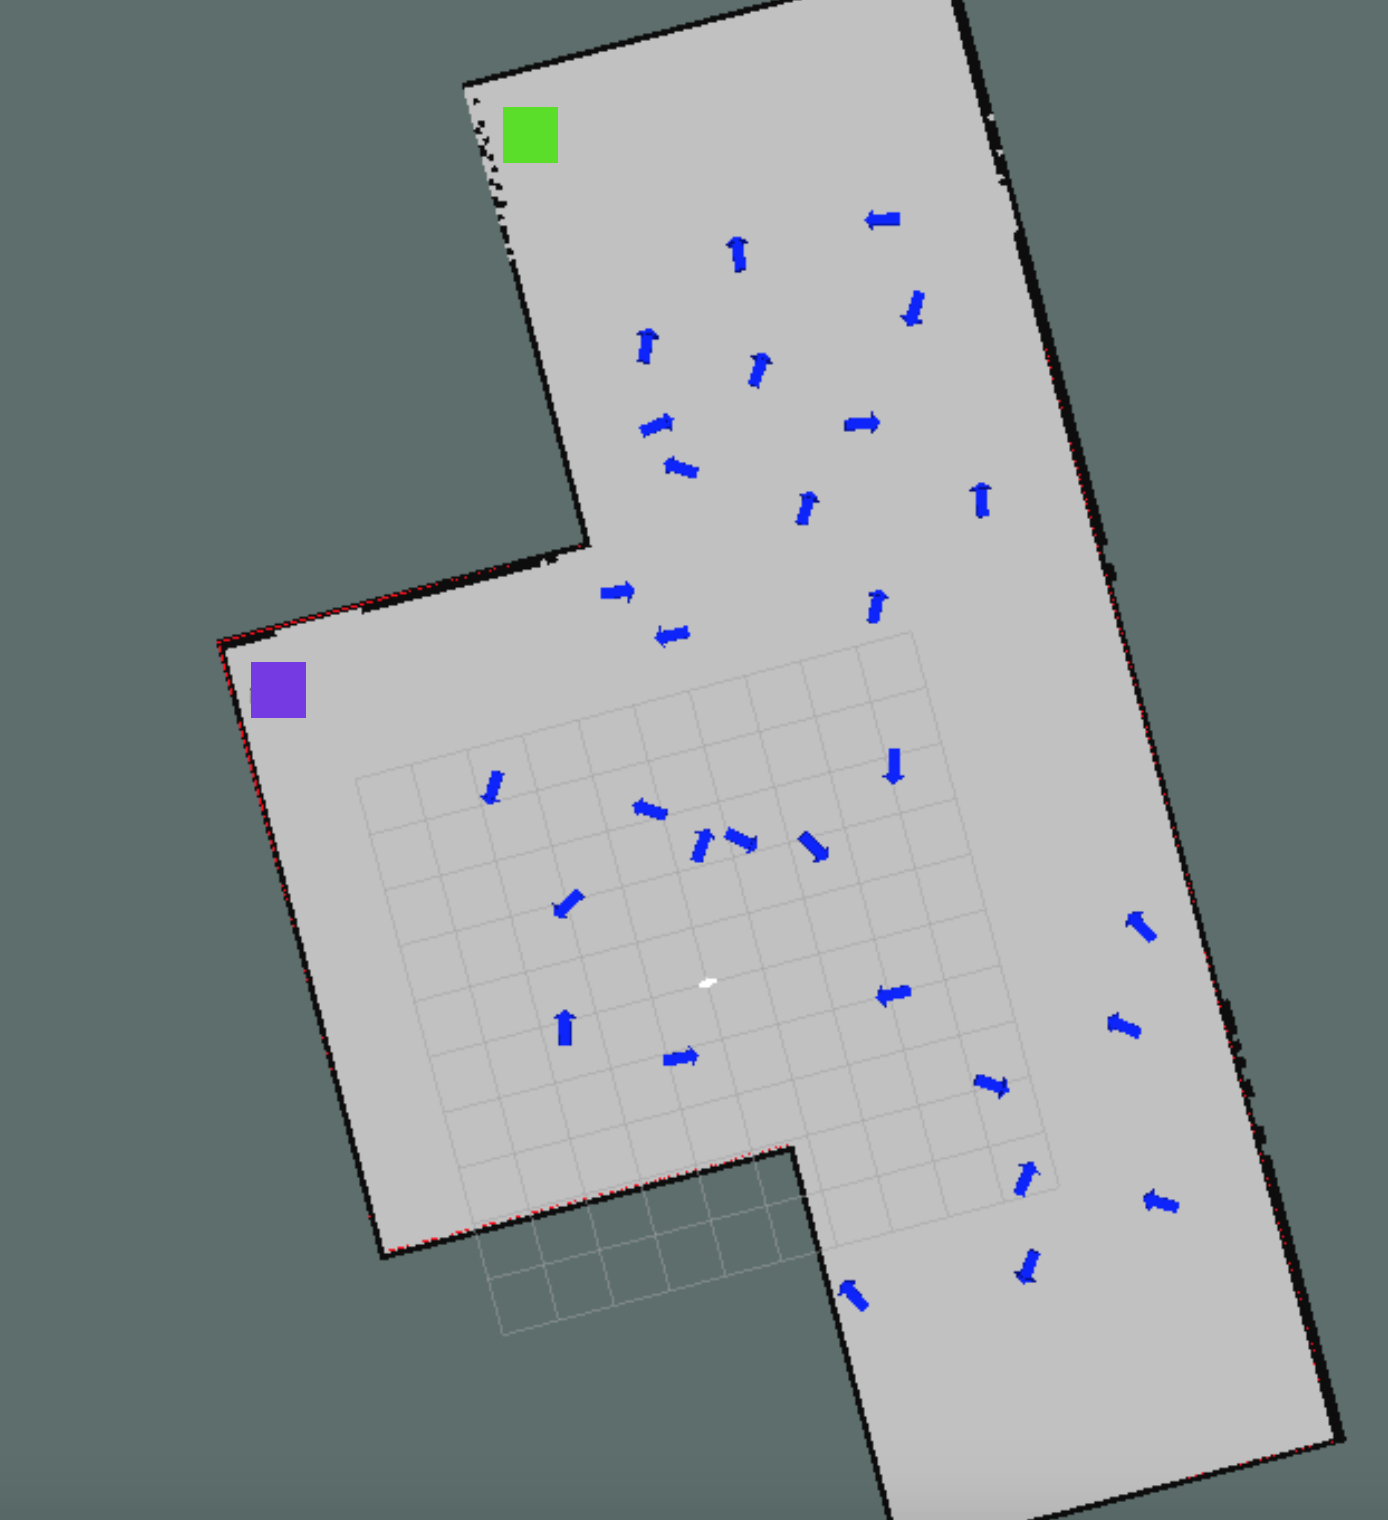
\includegraphics[scale = 0.15]{figures/no_cf.png}
    \caption{Example setting }
    \label{fig:exp_setting}
  \end{subfigure}
  \hspace{10mm}
  \begin{subfigure}[b]{0.35\columnwidth}
  \hspace{4mm}
    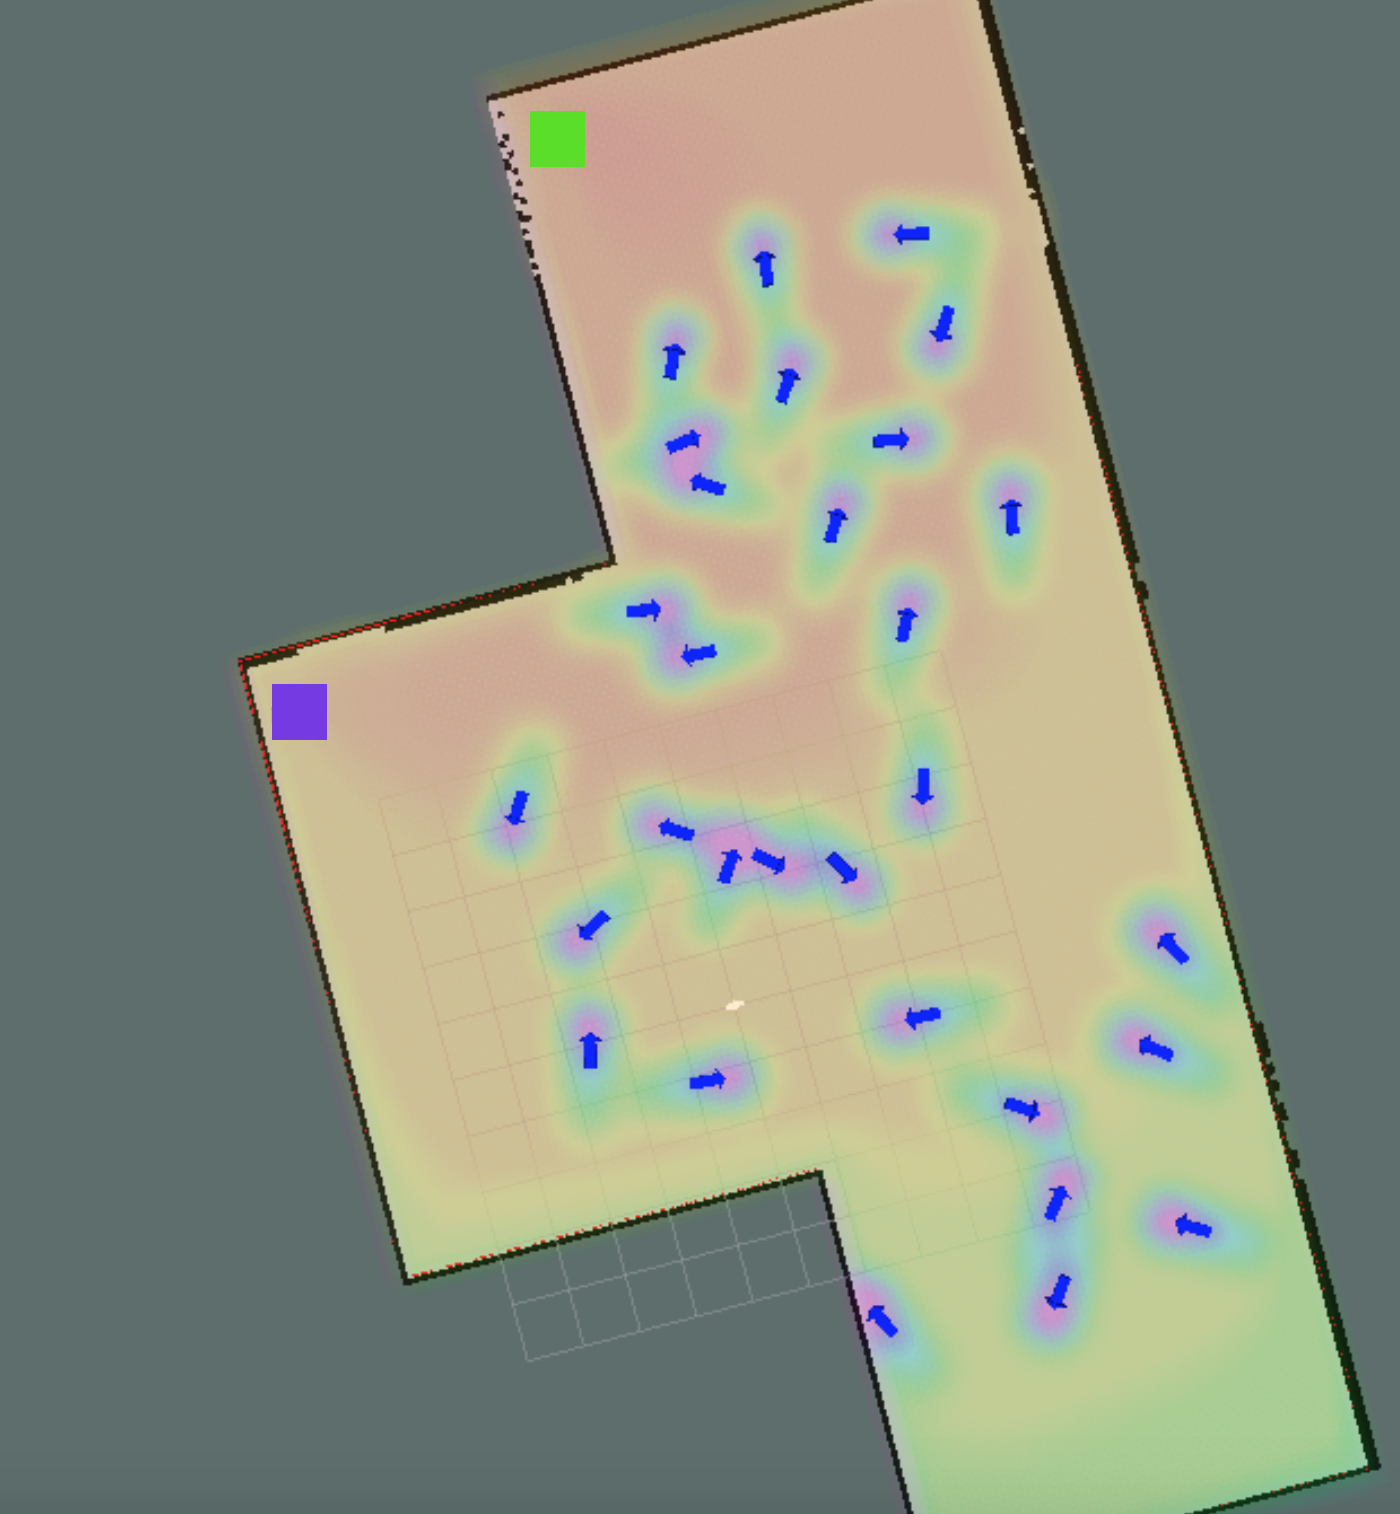
\includegraphics[scale = 0.15]{figures/cf.png}
    \caption{Cost function}
    \label{fig:cost_f}
  \end{subfigure} 

  %\vspace{-3mm}
  \caption[Simulated navigation task]{(a) A randomised instance of the social navigation task. Arrows denote the position and orientation of people in the scene. The robot is represented by the magenta box and the goal location is represented by the green box. (b) The corresponding cost function. Red denotes \emph{low} cost, while purple denotes \emph{high} cost.}

    \vspace{-2mm}

  %\vspace{-3mm}
  \label{fig:setting}
  \end{figure}

	The features we use can be divided into three categories. The first category encodes proxemics to the people present in the scene, i.e., the social features. Within this category we consider two variations, for reasons explained in the following section.
	\begin{itemize}
		\item {\bf Social feature set 1 (S1)}: Three isotropic Gaussian functions with different means, centred in front, behind, and on the person.
		\item {\bf Social feature set 2 (S2)}: Three field-of-view features. The features have a value of 1 if the robot is within a certain distance and angle from the person.
	\end{itemize}
	  The second category of features encodes the distance from the target location using linear, exponential, and logarithmic functions. The third category encodes the obstacle cost using a stable function of the reciprocal of the distance from the nearest obstacle. Figure \ref{fig:cost_f} shows an example cost function over the whole configuration space for the configuration in Figure \ref{fig:exp_setting}. We use different functions for human and target proximity, to allow for more degrees of freedom when modelling the underlying cost function. Sufficient regularisation ensures that that the model does not overfit.



% 	\begin{figure}[tbh]
% %	\hspace{-5cm}
% 	\centering
%       \begin{subfigure}[b]{0.42\columnwidth}
%     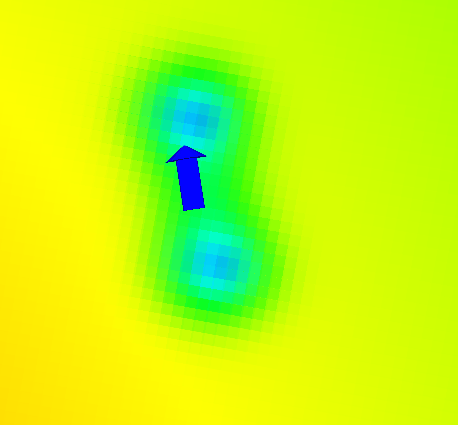
\includegraphics[scale=0.2]{images/person_feat2.png}
%     \caption{Social feature set S1.}
%     \label{fig:S1}
%   \end{subfigure}
%   \hspace{10mm}
%   \begin{subfigure}[b]{0.42\columnwidth}
%   \hspace{4mm}
%     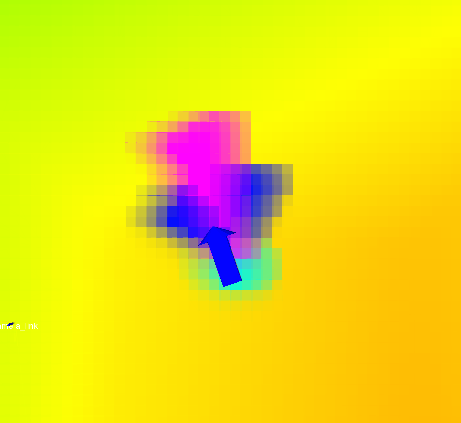
\includegraphics[scale=0.2]{images/person_feat1.png}
%     \caption{Social feature set S2}
%     \label{fig:S2}
%   \end{subfigure} 
%   %\vspace{-3mm}
%   \caption{Cost functions resulting from linear combinations of the social featuresets. Figure \ref{fig:S1} demonstrates featureset 1. It consists of three isotropic Gaussian functions centered in front in the center and behind the person. Figure \ref{fig:S2} shows the field-of-view features of featureset S2. \sw{I have no idea what these plots are showing.} \ks{Now?}}
%     \vspace{-2mm}
%   %\vspace{-3mm}
%   \label{fig:setting}
%   \end{figure}


	\subsubsection{Evaluation}

	To evaluate our algorithms, we generate a dataset $D$ by planning near-optimal paths from initial configurations $s_o$ to goal configurations $s_g$ under a ground-truth cost function $c_{gt}()$ derived from ground-truth weights $\mathbf{w}_{gt}$ and features $\mathbf{F}_{gt}$. A fully optimal path can only be derived asymptotically in terms of either time  for RRT$^*$, or resolution for A$^*$. In practice, however, we found that planning for 100 seconds using  RRT$^*$  achieves a path that is nearly optimal; running longer leads to negligible changes in path cost. 
	The resulting ground truth dataset enables a quantatitive empirical evaluation, which is otherwise problematic in IRL \cite{vasquez2014inverse,shiarlis2016inverse}. For each path $\zeta$ generated by the learning algorithm, we know its cost under the ground-truth cost function and features is simply  $\mathbf{w}_{gt}^T\mathbf{F}_{gt}(\zeta)$. Furthermore, we can compute the \emph{cost difference} between the learned path and the demonstrated path with respect to ground truth:
	\begin{equation}
		Q(\zeta,\zeta_i,\mathbf{w}_{gt}) = \mathbf{w}_{gt}^T(\mathbf{F}_{gt}(\zeta)-\mathbf{F}_{gt}(\zeta_i)), \label{eq:obj_eval}
	\end{equation}
which is our primary performance metric.  Note that, if the demonstration path $\zeta_i$ is optimal under $\mathbf{w}_{gt}$, then $Q(\zeta,\zeta_i,\mathbf{w}_{gt}) \geq 0$. For our holonomic simulated experiments, we consider two learning scenarios.
\begin{enumerate}
	\item \textbf{Unknown weights}: only $\mathbf{w}_{gt}$ is unknown. The demonstrations and the learning algorithm share social feature set S1.
	\item \textbf{Unknown weights and features}: $\mathbf{w}_{gt}$ and $\mathbf{F}_{gt}$  are unknown. S2 is used to generate the demonstrations and S1 is used for learning.
\end{enumerate}

The first scenario evaluates each algorithm's ability to learn good cost functions when provided only with limited demonstrations of the task. The second scenario introduces a feature discrepancy to better simulate real-world settings, since it is unlikely that the features we define will exactly match those implicitly used by the human demonstrator.
% In both cases the ground-truth weights $\mathbf{w}_{gt}$ were chosen to induce a cost function that penalises passing in front of people. In addition, small weights were added to the person related features, as well as linear and exponential penalisation of the distance from the goal, so that the cost functions would not be too trivial. 

We also document the total learning time for K iterations for the algorithms under comparison.  All algorithms were implemented in Python, share similar functions, and were not optimised for speed apart from the caching scheme in RLT$^*$. Finally, we perform a qualitative evaluation by visually comparing the learned cost functions for each algorithm and the paths they generate against ground truth.

	\subsubsection{Holonomic Robot Results}

	Our dataset $D$ consists of 20 trajectories from random social social situations. We split $D$ into $D_{train}$ and $D_{test}$, each with 10 trajectories. After training on $D_{train}$, the cost difference of a cost function is evaluated on $D_{test}$ using \eqref{eq:obj_eval}. The process is repeated 7 times for the same dataset but with different random compositions of $D_{train}$ and $D_{test}$.  All learning algorithms are initialised using the same cost function that only favours shortest paths.
	
	As mentioned earlier, planning time and grid resolution affect the performance of RRT$^*$ and $A^*$, respectively. To make a fair comparison, we vary these two quantities for each algorithm and plot cost difference against learning time at each setting.  We can then identify which algorithms at which settings comprise the Pareto front, i.e., are undominated with respect to cost difference and learning time.
	
	 Figures \ref{fig:res_sim1} and \ref{fig:res_sim2} show the results for the two scenarios described earlier. MMP\_X (green) refers to MMP with X meters of grid resolution while  RLT\_X (red) and RLT$^*$-NC\_X (blue) refer to RLT and RLT without caching, respectively, with X seconds of planning. The shading represents an interpolation of the performance between settings for each method. In this way an area of single colour illustrates hypothesized domination of that method over another, given the same amount of time. Since lower is better for both cost difference and learning time, the closer a point is to the bottom left corner, the better.

	\begin{figure}[tbh]
	\centering
	\captionsetup[subfigure]{justification=centering}
	\hspace{-1cm}
      \begin{subfigure}[b]{0.41\columnwidth}
    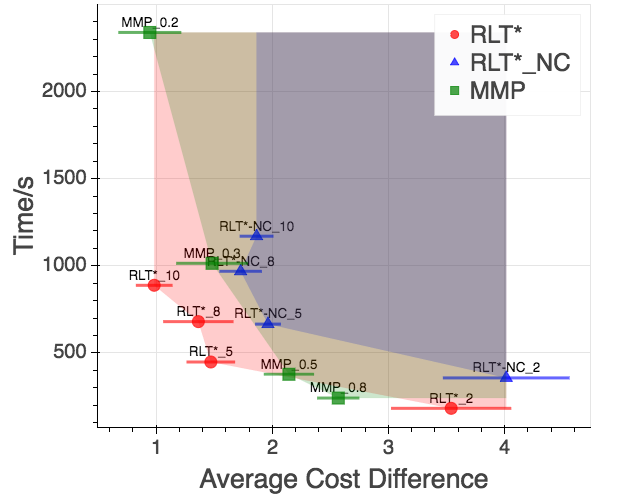
\includegraphics[scale=0.40]{figures/pf_same.png}
    \caption{Unknown weights scenario.}
    \label{fig:res_sim1}
  \end{subfigure}
     	\hspace{10mm}
  \begin{subfigure}[b]{0.41\columnwidth}

    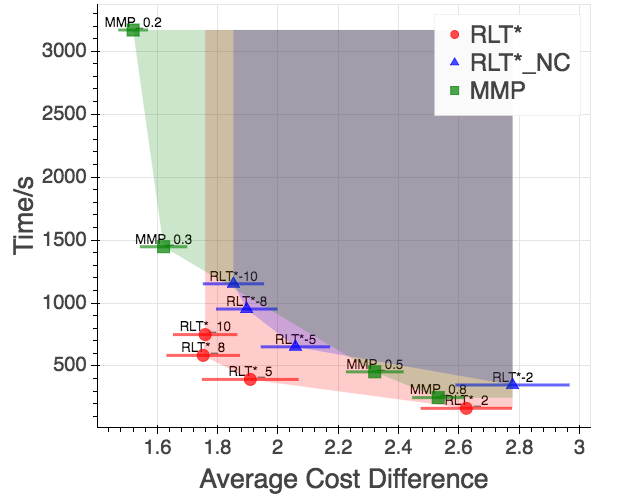
\includegraphics[scale=0.40]{figures/pf_different.png}
    \caption{Unknown weights and features scenario.}
    \label{fig:res_sim2}
  \end{subfigure} 
    \caption[Learning time vs.\ cost difference on the holonomic robot]{Learning time vs.\ cost difference on the holonomic robot for MMP (green), RLT$^*$-NC (blue), and RLT (red) at different planning fidelities. On both axes \emph{lower is better}.}
    \vspace{-2mm}
  %\vspace{-3mm}
  \label{fig:results_sim}
  \end{figure}

 RLT$^*$ (red) comprises a large majority of the Pareto front, demonstrating good performance and generalisation in reasonable time.  However, the performance of RLT$^*$ and RLT$^*$-NC significantly degrades at very low planning times (2 seconds) because AMMP cannot sample good enough paths to compute a useful gradient.
 
 Note that caching not only speeds learning in RLT$^*$, it also modestly reduces cost differences. This suggests that the caching scheme introduces extra robustness and generalisation capabilities within the algorithm.  As mentioned in Section \ref{subsec:cached}, we hypothesise that the caching scheme improves learning by making the gradients smoother and more consistent, as with momentum. To confirm this, we plot the inner product between successive gradients during learning in Figure \ref{fig:in_prod_grad}. The plot confirms that subsequent gradients in RLT$^*$ are more similar.
 
 Finally, note that MMP's learning time scales exponentially with the size of the grid. This, however, is not solely due to the graph getting larger but also because A$^*$ search scales poorly with the complexity of the cost function itself. Since it relies on an admissible heuristic that for complex cost functions is no longer tight, A$^*$ must expand many more states.  RLT$^*$ is less susceptible to such problems.

 	\begin{figure}[tbh]
%	\hspace{-5cm}
	\centering
    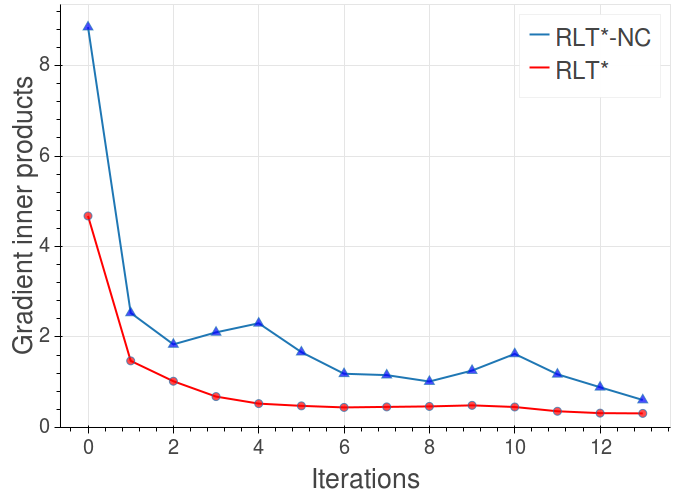
\includegraphics[scale=0.40]{figures/momentum.png}
    \caption[Inner product of succcessive gradients during learning]{Inner product of succcessive gradients during learning. The smoother curve for RLT$^*$ suggests that fixing the sampled points during learning makes the gradients more consistent. }
    \vspace{-2mm}
  %\vspace{-3mm}
  \label{fig:in_prod_grad}
  \end{figure}


  \subsubsection{Non-Holonomic Robot Results}
  As mentioned earlier, a potential advantage of RLT$^*$ is that it can efficiently handle learning in the presence of motion constraints. In this section, we consider a robot planning in a three-dimensional space, $(x,y,\theta)$, representing the position and orientation of the robot. The robot's motion is further subject to the following motion constraints:
%
  \begin{align}
  	&\dot{x} = v\times\cos(\theta),\\
  	&\dot{y} = v\times\sin(\theta),\\
  	&\dot{\theta} = \omega,
  \end{align}
  where $v,\omega$ are the linear and angular velocities respectively.
  To meet these constraints, we use the POSQ $\texttt{Steer}$ function \cite{palmieri2014novel}.  Since this approach gives a local closed-loop policy between two vertices of the tree, it is  more robust to noise and uncertainty in the motion than an open loop trajectory. Furthermore, it has been shown to produce smooth paths between feasible configurations \cite{palmieri2014novel}. Evaluation is done in the same way as in the previous section, except that we compare RLT$^*$ only to RLT$^*$-NC and not MMP, as the latter cannot handle motion constraints.
RLT$^*$-NC was given 100 seconds to plan, in which case about 3000 configurations were sampled, and RLT$^*$'s cache was set to this size. 

Figure \ref{fig:results_kino} shows that RLT$^*$ is an order of magnitude faster than RLT$^*$-NC, while achieving a lower cost difference. The kinematic constraints contribute to this speedup since they make the \texttt{Steer} and \texttt{Safe} procedures, which are cached, more expensive. As in the holonomic case, RLT$^*$ resulted in smoother learning, confirming the results of Figure \ref{fig:in_prod_grad}. 

  	\begin{figure}[tbh]
	\centering
	\captionsetup[subfigure]{justification=centering}
	\hspace{-1cm}
      % \begin{subfigure}[b]{0.42\columnwidth}
    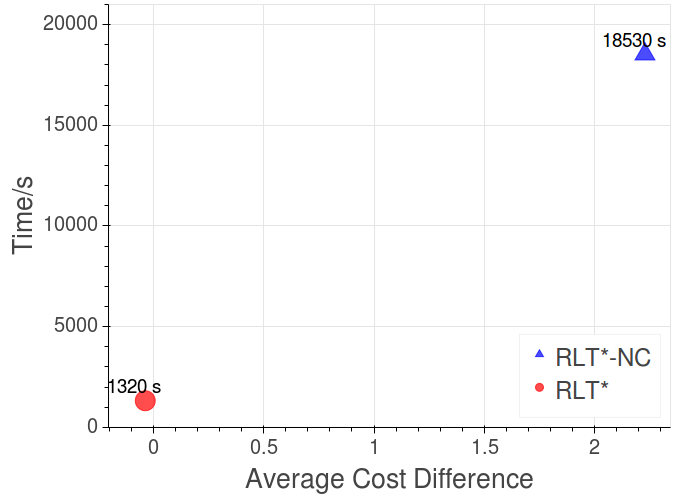
\includegraphics[scale=0.4]{figures/pareto_front_kino.png}
    % \caption{Learning time vs.\ cost difference.}
    % \label{fig:res_kino1}
  % \end{subfigure}
     	% \hspace{10mm}
  % \begin{subfigure}[b]{0.42\columnwidth}

  %   \includegraphics[scale=0.25]{images/cost_diff_val_kino.png}
  %   \caption{Learning curve}
  %   \label{fig:res_kino2}
  % \end{subfigure} 
    \caption{Non-holonomic robot results.}
    \vspace{-2mm}
  %\vspace{-3mm}
  \label{fig:results_kino}
  \end{figure}

Figure \ref{fig:results_qual} shows an instance of the types of paths generated by our method when compared to ground truth. This specific example was drawn from the validation set and is thus not a case of overfitting.


	\begin{figure}[tbh]
%	\hspace{-5cm}
	\centering
    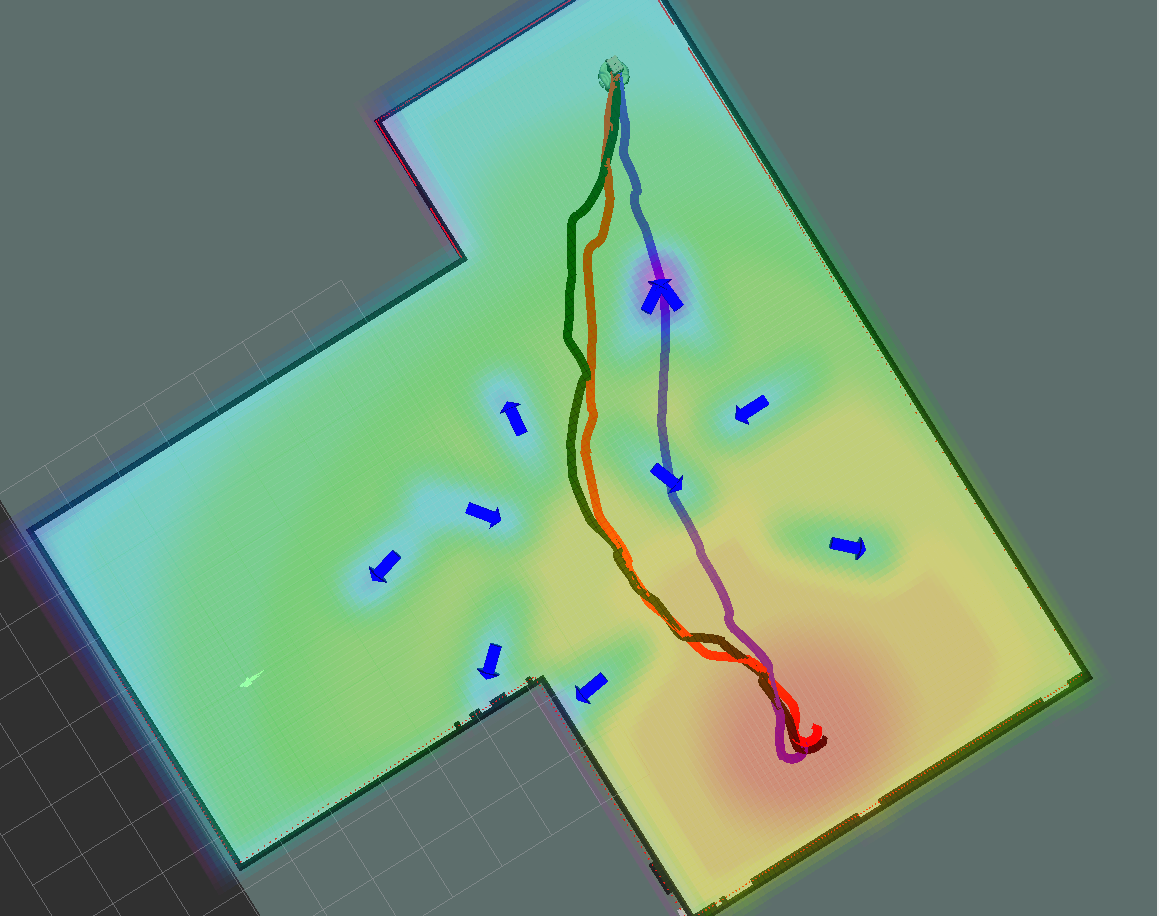
\includegraphics[scale=0.15]{figures/kino_paths.png}
    \caption[Qualitative comparison of simulated results]{Qualitative evaluation of simulated results. The colour map denotes the learned cost function. Red denotes \emph(low) cost and green \emph{high} cost. The learned path (red) is quite similar to the demonstrated path (black) with a clear improvement over the path before learning (purple).}
    \vspace{-2mm}
  %\vspace{-3mm}
  \label{fig:results_qual}
  \end{figure}

	\subsubsection{Real Robot Experiments}
	In this section, we apply RLT$^*$ to real, human demonstrations the TERESA robot, in a social navigation scenario. Furthermore, we deploy the learned cost function on the actual robot.

We use the data collected during local experiments at the UPO during October and November 2015. This dataset is explained in a previous deliverable (D5.1). RLT$^*$ learns a cost function from this data using the social feature set S1 and the rest of the features described earlier.

Since quantitative evaluation is difficult using real data, as no ground truth is available, we perform a qualitative evaluation instead. Figure \ref{fig:results_real} shows some representative cases that arose during learning. Figure \ref{fig:res_real1} shows a case where RLT$^*$ produced paths (red) that are quite similar to the demonstrated ones (black). Figure \ref{fig:res_real4} shows an instance instances where  the learned paths are reasonable even though they are not similar to the demonstrated paths.

			\begin{figure}[tbh]
	\centering
      \begin{subfigure}[b]{0.42\columnwidth}
    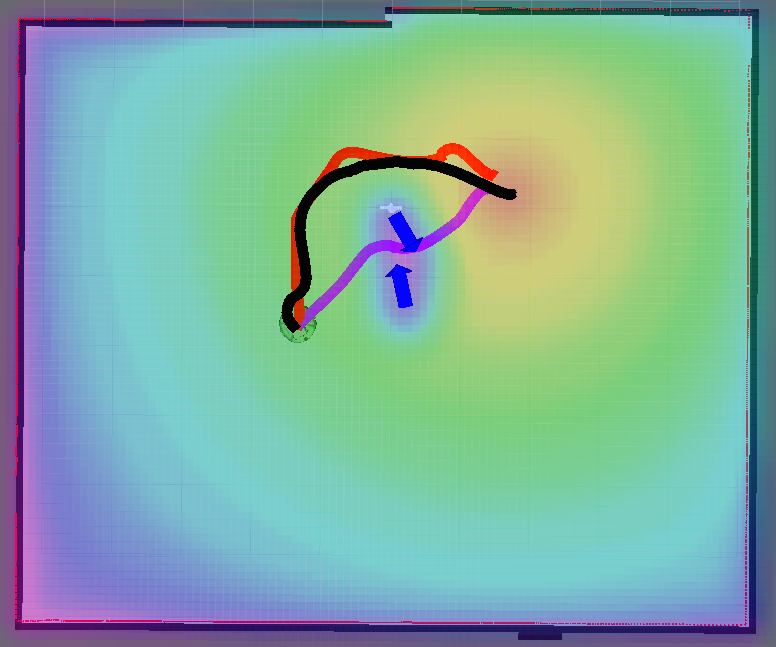
\includegraphics[scale=0.20]{figures/real_good_new.png}
    \caption{}
    \label{fig:res_real1}
  \end{subfigure}
  \begin{subfigure}[b]{0.42\columnwidth}
    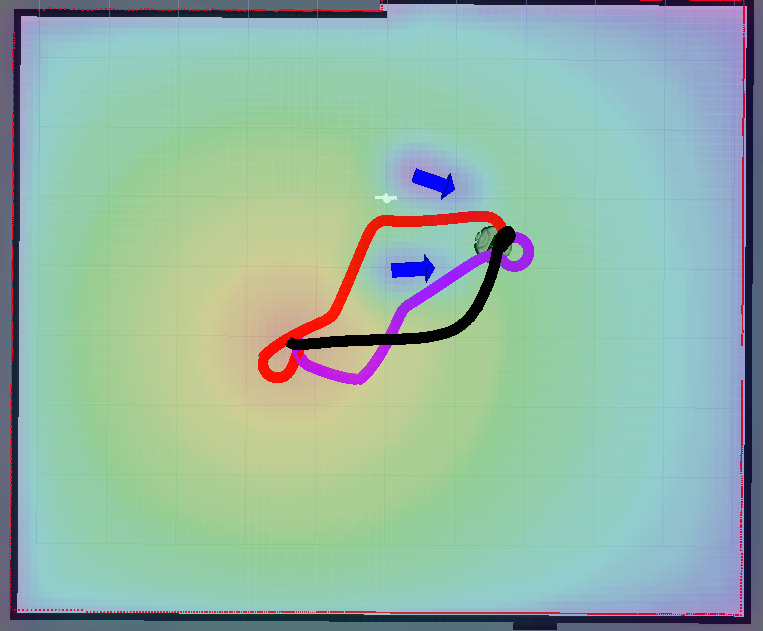
\includegraphics[scale=0.20]{figures/real_reasonable_new.png}
    \caption{}
    \label{fig:res_real4}
  \end{subfigure} 
    \caption[Real vs learned paths]{Real demonstrated paths (black), learned paths (red), and shortest paths (purple). In (a), the learned path is similar to the demonstrated path; in (b) it is different but reasonable. The paths are laid over the learned cost function.}
  \label{fig:results_real}
  \end{figure}


	Finally, we successfully deployed the learned cost function, also shown in Figure \ref{fig:results_real}, on a real telepresence robot. A video demonstrating this deployment can be found in the supplementary material. Even though our planner outputs a full policy in terms of angular and linear velocities, to follow the prescribed path we used an elastic bands local planner in order to deal with dynamic changes in the environment.



\vspace{-1mm}
\subsection{Conclusion \& Future Work}
In this paper, we proposed Rapidly Exploring Learning Trees (RLT$^*$), which learns the cost functions of Rapidly Exploring Random Trees (RRT) from demonstration, thereby making inverse learning methods applicable to more complex tasks. Our approach extends the Maximum Margin Planning to work with RRT$^*$ cost functions. Furthermore, it uses a caching scheme that greatly reduces the computational cost and improves performance. Our results in simulated social navigation scenarios show that RLT$^*$ achieves better performance at lower computational cost, even when there is a discrepancy between the features used for demonstration and learning. Furthermore, our results show that RLT$^*$ can handle more complex configuration spaces with motion constraints. Finally, we used RLT$^*$ to learn a cost function using data from real demonstrations from the TERESA robot and successfully deployed that cost function.

In future work, we hope to extend RLT$^*$ to model how features evolve over time, in order to, e.g., consider people's movement during planning.  For complex social path planning applications, periodic replanning has been shown to help \cite{henry2010learning,vasquez2014inverse}. Replanning in RRT$^*$ is also possible \cite{otte2015rrtx} and could potentially be incorporated into RLT$*$.
=======
Learning from demonstration (LfD) \cite{argall2009survey} is of great interest to roboticists because it can circumvent tedious and often infeasible manual programming of complex behaviours. While most LfD methods rely on supervised learning (i.e., behavioural cloning) to directly learn policies, certain approaches, namely inverse optimal control (IOC) \cite{kalman1964linear} and inverse reinforcement learning (IRL) \cite{abbeel2004apprenticeship} instead learn \emph{cost functions} from demonstration, which are then used to \emph{plan} the robot's behaviour. 

In addition, learned cost functions are often useful even when the environment changes.  For example, if the friction in a robot's wheels changes due to wear and tear, the optimal policy will change but the cost function will not. Thus, a robot trained via supervised learning would need to learn a new policy, while a robot trained via IRL could simply replan on the new dynamics with its existing cost function. In addition, cost functions are thought to be more succinct representations of the aims of the agent \cite{abbeel2004apprenticeship}. For example, a robot whose aim is to reach a goal as fast as possible may have a simple cost function but a complex policy. 

IRL is an iterative process that, in an inner loop, solves the forward planning problem (i.e., finds an optimal policy under the current cost function) and subsequently, in an outer loop, updates the current cost function. This process repeats until convergence. For continuous domains such as robotics, solving the planning problem exactly is typically intractable. Doing so may result in high-dimensional models to which most planning algorithms scale poorly, necessitating a coarse discretisation that yields poor performance.  Consequently, in robotics, planning is often done using sample-based, single-query motion planners such as Rapidly Exploring Random Trees (RRTs) \cite{lavalle1998rapidly} and their variants \cite{karaman2011sampling}. Such methods can cope with high-dimensional continuous domains, as well as the presence of obstacles in the environment and motion constraints on the robot.


In this paper, we first propose Approximate Maximum Margin Planning (AMMP), a variant of Maximum Margin Planning (MMP) \cite{ratliff2006maximum} that does not assume an optimal planner. Doing so allows us to use sample-based planning algorithms, such as RRT$^*$ in the inner loop of IRL. Second, we propose a caching scheme that both improves performance and reduces the computational cost when RRT$^*$ is used within AMMP. The resulting algorithm, which we call Rapidly Exploring Learning Trees (RLT$^*$),  allows computationally efficient IRL in high-dimensional, continuous domains with obstacles and motion constraints. 

We evaluate RLT$^*$ on real and simulated data from a social navigation scenario. The results demonstrate that, in the absence of obstacles and motion constraints, RLT$^*$ performs better and is faster than both MMP and RLT$^*$ without caching. Furthermore, we show that RLT$^*$, unlike MMP, can learn cost functions in robotic tasks with obstacles and motion constraints. Finally, we deploy our method on a real telepresence robot using data from human demonstrations.

\subsubsection{Related Work \label{sec:related_work}}


Substantial research has applied IRL to robotics \cite{henry2010learning,abbeel2008apprenticeship,vasquez2014inverse}.
A big challenge in doing so is solving the forward planning problem under the current cost function at every iteration. The planning problem is especially intractable in robotics because the state-action spaces encountered are often continuous and high dimensional. 
One approach is to discretise the state-action spaces and solve the resulting Markov decision process (MDP). However, in high-dimensional tasks, fine discretisations render planning intractable and coarse discretisations yield poor performance.

Some methods that use discretisation formulate the problem such that only an open-loop path (rather than a closed-loop policy) is required. Then, given deterministic dynamics, planning can be performed using A$^*$ \cite{ratliff2006maximum}, allowing realistic problems to be tackled. We take a similar approach but, by planning using RRT$^*$, we substantially enlarge the class of tasks that can be tackled.

Another approach is to use hybrid planners. Inverse Optimal Heuristic Control \cite{ratliff2009inverse} models the long-term goals of the agent as a coarsely discretised MDP, to ensure tractability, while using supervised learning to determine the local policy of the agent at each state. Graph-Based IOC \cite{byravan2015graph} uses discrete optimal control on a coarse graph and the actual path is executed using local trajectory optimisation techniques such as CHOMP \cite{ratliff2009chomp}, which would otherwise suffer from local minima. However, these methods employ complex and domain-specific planning formulations that are not suitable for all robotics tasks. By contrast, our approach employs a widely used planner, making it versatile and easy to implement. 

Another recent method is Adaptive State Graphs \cite{okallearning}, which builds a state-action controller graph before doing any learning. This controller graph is akin to \emph{options} in semi-Markov decision processes, and allows for a more flexible representation of the state-action space. However, the controller used to learn the underlying cost function is different from the one used to execute the robot's behaviour. This can have adverse effects since IRL  assumes that the demonstration paths came from the same planner used during learning.  Instead of building a controller graph first and then using a different controller to optimise trajectories, RLT$^*$ builds a controller tree on the fly and uses the same planner for learning and execution.

All of the above methods require a model of the dynamics of the system. Another paradigm, that of model-free IRL, avoids the need to explicitly plan, employing sampling instead. As a result it tends to scale better to high-dimensional state-action spaces and does not require a model of the system dynamics, \cite{boularias2011relative,kalakrishnan2013learning}.
 Model free IRL samples trajectories, usually starting from the initial conditions observed in the data. The probability of these trajectories is weighted according to the current cost function, which is then updated to make trajectories closer to the data more likely. A big challenge is to find an appropriate importance distribution at each iteration. \cite{finn2016guided} considers guiding the importance distribution by simultaneously learning a good policy under the current cost function and using it as an adaptive importance sampler. However, since it uses a modified version of Linear Quadratic Regulator control the derived policies are only locally optimal and can produce highly suboptimal paths or even fail in the presence of obstacles. By contrast, RRTs cope naturally with obstacles, as long as they are static and mapped, and is also asymptotically optimal.

\subsection{Background}
We begin with background on path planning and inverse reinforcement learning for path planning.

\subsubsection{Path Planning \label{subsec:path_planning}}
Path planning occurs in a space $\mathcal{S}$ of possible robot configurations. A configuration $s \in \mathcal{S}$ is usually continuous, and often represents spatial quantities such as position and orientation. A path planner seeks an obstacle-free path $\zeta_{o,g} = (s_1,s_2,s_3$ $\ldots,s_{l_{\zeta}}) $ of length $l_{\zeta}$, from an initial configuration $o = s_1$ to a goal configuration  $g =s_{l_{\zeta}}$. When the initial and goal configurations are implied, we refer to a path as $\zeta$.

As there could be several paths to the goal, planners often employ a \emph{cost functional}, $C(\zeta)$, which typically sums the costs between two subsequent configurations $c(s_i,s_j)$:
\begin{equation}
	C(\zeta) = \sum_{i=1}^{l_{\zeta}-1} c(s_i,s_{i+1}).
\end{equation}
This cost functional is similar to the one used in optimal control and analogous to the return used in reinforcement learning. Given the cost functional, the path planner seeks an optimal path $\zeta^*$, which satisfies,
\begin{equation}
 	\zeta^*_{o,g} = \argmin_{\zeta_{o,g} \in Z_{o,g}} C(\zeta), \label{eq:back_plan}
\end{equation}
where $Z_{o,g}$ is the set of possible paths such that $s_1 = o, s_{l_\zeta} = g$. Many path planning algorithms discretise $\mathcal{S}$ and use graph search algorithms like A$^*$ to find the optimal path. Under mild assumptions, these approaches are guaranteed to find the best path on the graph, therefore solving \eqref{eq:back_plan} for a subset $\tilde{Z}_{o,g} \subset Z_{o,g}$, whose size depends on the discretisation. However, such methods scale poorly in the size of $\mathcal{S}$. Furthermore, such algorithms ignore motion constraints as they assume all nodes in the graph can be reached by their neighbours in exactly the same way. This assumption does not hold, e.g., for non-holonomic robots, where the ortientation at each node places constraints on how it can be reached. In this constrained space, it is less straightforward to define actions, neighbouring nodes, or an admissible heuristic, which is necessary for optimality.

These drawbacks motivate \emph{sample-based} path planning algorithms such as RRT$^*$  \cite{karaman2011sampling}. Instead of building a graph and then searching it, RRT$^*$ builds a tree on the fly and keeps track of the current best path. The algorithm consists of two interleaved steps. 

The first step is \emph{sampling}. A random point $s_{rand}$ is sampled from the configuration space. Next, the closest point $s_{closest}$, already in the existing vertex set $V$ is determined and a new point $s_{new}$ is created by \emph{steering} from  $s_{closest}$ to $s_{rand}$. In a Euclidean space, steering between two points means simply connecting them with a straight line. However, if orientations and motion constraints are used, then becomes more complex. Finally, the sampling step determines the points, $S_{near}$, within a given radius of $s_{new}$.

The second step is \emph{rewiring}, which determines which points in $S_{near}$ we should connect to $s_{new}$, i.e., it determines which path to $s_{new}$ results in a lowest cost path. Finally, we repeat this step for the parents of $S_{near}$. Thus, the tree is rewired locally around the new point, such that lower global cost paths arise.

Alternating between these two steps for a given time budget $T$ solves \eqref{eq:back_plan} for a subset $\tilde{Z}_{o,g}$ that is determined by the randomly sampled points. As $T \rightarrow \infty$, RRT$^*$ minimises over the entire $Z_{o,g}$, i.e., it is asymptotically optimal in time \cite{karaman2011sampling}. By contrast, A$^*$ is asymptotically optimal in resolution.


\subsubsection{IRL for Path Planning \label{subsec:inverse_problem}}
In path planning, we are given a cost function and must find a (near) optimal path to the goal. In the inverse problem, we are given example paths and must find the cost function for which these paths are (near) optimal.  The example paths comprise a dataset $\mathcal{D} = (\zeta^1_{o_1,g_1},\zeta^2_{o_2,g_2}...\zeta^D_{o_D,g_D})$ where $\zeta^i_{o_i,g_i}$ is an example path with initial and final configurations $o_i$ and $g_i$. We assume the unknown cost function is of the form,
\begin{equation}
	c(s_i,s_j) = \mathbf{w}^T \mathbf{f}(s_i,s_j), \label{eq:inner_prod}
\end{equation}
where $\mathbf{f}(s_i,s_j)$ is a $K$-dimensional vector of features that encode different aspects of the configuration pair and $\mathbf{w}$ is a vector of unknown weights to be learned. Since $\mathbf{w}$ is independent of the configuration, we can express the total cost of the path in a parametric form:

\begin{equation}
	C(\zeta) = \mathbf{w}^T\sum_{i=0}^{l_{\zeta}-1} \mathbf{f}(s_i,s_{i+1}) := \mathbf{w}^T \mathbf{F}(\zeta),
\end{equation}
where $\mathbf{F}(\zeta)$ is the \emph{feature sum} of the path.

While many formulations of the inverse problem exist, the general idea is to find a weight vector that assigns less cost to the example paths than all other possible paths with the same initial and goal configuration.  This can be formalised by a set of inequality constraints:

\begin{equation}
	C(\zeta^i_{o_i,g_i}) \leq  C(\zeta) \quad \forall \zeta \in Z_{o_i,g_i}  \quad \forall i. \label{eq:const1}
\end{equation}
The constraint is an inequality because $Z_{o_i,g_i}$ contains only paths available to the planner and thus may not include the example path $\zeta^i_{o_i,g_i}$.
$Z_{o_i,g_i}$ can be large but if we have an optimisation procedure that solves \eqref{eq:back_plan}, it is enough to satisfy, 
\begin{equation}
	C(\zeta^i_{o_i,g_i}) \leq \min_{\zeta \in Z_{o_i,g_i}} C(\zeta) \quad \forall i. \label{eq:const}
\end{equation}

Maximum Margin Planning (MMP) \cite{ratliff2006maximum} introduces a margin function $L_i(\zeta)$ that decreases the cost of the proposed path $\zeta$ if it is dissimilar to $\zeta^i_{o_i,g_i}$. For example, $L_i(\zeta)$ could be $-1$ times the number of configurations in the demonstration path not visited by $\zeta$. As in Support Vector Machines, requiring the model to fit the data well even in the presence of a margin improves generalisation. Furthermore, the margin helps address the ill-posed nature of IRL, i.e., many cost functions are consistent with the demonstrated behaviour. Formally, MMP solves the following optimisation problem:
\begin{equation}
	\argmin_{\mathbf{w},\tau} \frac{1}{2}||\mathbf{w}||^2 + \frac{\lambda}{D} \sum_i \tau_i \label{eq:mas_marg}
\end{equation}
\begin{equation}
	\text{s.t.} \quad C(\zeta^i_{o_i,g_i}) - \tau_i \leq \min_{\zeta \in Z_{o_i,g_i}} C(\zeta) + L_i(\zeta) \quad \forall i,
\end{equation}
where $\tau_i$ are slacks that can be used to relax the constraints. Rearranging the inequality in terms of the slacks yields:

\begin{equation}
	 \quad C(\zeta^i_{o_i,g_i}) - \min_{\zeta \in Z_{o_i,g_i}} C(\zeta) + L_i(\zeta)  \leq \tau_i  \quad \forall i.
\end{equation}
Consequently, the $\mathbf{w}$ minimising:
\begin{equation}
	\frac{1}{2}||\mathbf{w}||^2 + \frac{\lambda}{D} \sum_i \big( C(\zeta^i_{o_i,g_i}) - \min_{\zeta \in Z_{o_i,g_i}}\big(C(\zeta) + L_i(\zeta)\big) \big) \big. \label{eq:unconstrained}
\end{equation}
also minimises \eqref{eq:mas_marg}, i.e., the slacks are tight.
The minimum can be found by computing a subgradient and performing gradient descent on the above objective:
\begin{equation}
	\nabla_{\mathbf{w}} =\mathbf{w} +  \frac{\lambda}{D} \sum_{i=0}^D F(\zeta^i_{o_i,g_i}) - F(\tilde{\zeta}^*_{o_i,g_i}), \label{eq:update1}
\end{equation}
where,
\begin{equation}
	\tilde{\zeta}^*_{o_i,g_i} = \argmin_{\zeta \in Z_{o_i,g_i}} C(\zeta) + L_i(\zeta). \label{eq:augmented_max}
\end{equation}

The inverse problem can therefore be seen as an iterative procedure that first solves \eqref{eq:augmented_max} in the inner loop while keeping the weights constant. Given that solution, it then updates the weights using \eqref{eq:update1} in the outer loop. The weights at convergence represent the cost function that is used to plan future behaviour. In \cite{ratliff2006maximum}, A$^*$ search was used for planning in the inner loop, assuming that the domain contained acyclic positive costs. In this paper, we make the same assumptions but develop methods that use RRT$^*$ for planning.

\subsection{Method}
	In this section, we propose Rapidly Exploring Learning Trees (RLT$^*$).  We first propose a generic extension to MMP that we call Approximate Maximum Margin Planning.  We then show how an implementation of this approach with an RRT$^*$ planner and a novel caching scheme yields RLT$^*$.

	\subsection{Approximate Maximum Margin Planning \label{subsec:ammp}}

Section \ref{subsec:inverse_problem} shows how the multiple constraints of \eqref{eq:const1} can be reduced to the single constraint of \eqref{eq:const} for each demonstration. However, this reduction requires an optimal planner to perform the minimisation in \eqref{eq:const1}, which is impractical in many robot applications. Suppose instead that, as in RRT$^*$, we have a mechanism for sampling different paths from $Z_{o,g}$ along with their respective costs and that, for a given finite time budget $T$, this path sampler samples a subset $\tilde{Z}_{o,g} \subset Z_{o,g}$,  Then, we can modify \eqref{eq:const} to demand that our cost function satisfies,
\begin{equation}
	C(\zeta^i_{o_i,g_i}) \leq \min_{\zeta_{o_i,g_i} \in \tilde{Z}_{o_i,g_i}} C(\zeta) \quad \forall i. \label{eq:const_rrt}
\end{equation}
	As $T$ increases, lower cost paths are sampled, making this inequality harder to satisfy. Assuming $\tilde{Z}_{o_i,g_i}$ is constant, we can rewrite \eqref{eq:unconstrained} as:

	\begin{equation} \frac{1}{2}||\mathbf{w}||^2 + \frac{\lambda}{D} \sum_i \big( C(\zeta^i_{o_i,g_i}) - \min_{\zeta \in \tilde{Z}_{o_i,g_i}}\big(C(\zeta) + L_i(\zeta)\big) \big). \label{eq:unconstrained_rrt}
	\end{equation}
This gives rise to an approach we call Approximate Maximum Margin Planning (AMMP). It is similar  to MMP with the crucial difference that the planning step is executed by a sample-based planner and not a deterministic one, like A$^*$. An important consequence is that $\tilde{Z}_{o_i,g_i}$ changes every time we invoke the sample-based planner. Thus, AMMP can be thought of as sampling the \emph{constraints} that we want our cost function to satisfy. The main advantage of AMMP is that it is not bound by the restrictive assumptions of  A$^*$, such as a discrete state-action space and no motion constraints. 

However, an ineffective sampler could yield poor gradient estimates and thus poor solutions. In fact, Ratliff et al.\ \cite{ratliff2009chomp} argue that, for this reason, sample-based planners like RRT are not suited to learning cost functions from demonstration, as the paths sampled by RRT are heavily biased during the sampling process and thus highly suboptimal. However, asymptotically optimal sample-based planners like RRT$^*$ are better able to plan low-cost paths \cite{karaman2011sampling} and thus well suited for use within AMMP.

\subsubsection{Rapidly Exploring Learning Trees \label{subsec:cached}}

As suggested above, a simple way implement AMMP is to use RRT$^*$ as the sample-based planner.  RRT$^*$ can sample low-cost paths, allowing AMMP to learn a good cost function. Furthermore, RRT$^*$ can cope with large and continuous state-action spaces with motion constraints. However, the result is a computationally expensive algorithm that calls the planner $I\times|D|$ times over $I$ iterations, given a dataset of size $|D|$. Furthermore, sampling a separate set of points at every iteration could produce noisy gradients that negatively affect convergence. In this section, we propose Rapidly Exploring Learning Trees (RLT$^*$), which implements AMMP with an RRT$^*$ planner using a novel caching scheme to ensure both computational efficiency and more consistent gradients.

A key observation is that, in RRT$^*$, only the rewiring step depends on the cost function.  The sampling step is independent of it and, especially when motion constraints are present, contains the most computationally expensive operations. These are: 1) fitting and querying a data structure to find the nearest neighbour and the radius neighbours to a newly sampled point, 2) applying the steer function to all neighbours to and from the newly sampled point, and 3) checking for obstacles in these paths. By contrast,  the only potentially expensive operation in the rewiring step is querying the cost of an edge. 

Therefore, a key idea behind RLT$^*$ is to perform the sampling step just once for each data point and cache it for reuse throughout learning. Then, at each iteration, only the rewiring step needs to be repeated as the cost function changes.

Algorithm \ref{alg:rrt_cache} describes the caching step, which takes as input $p$, the number of points to randomly sample from free space; $s_{init}$, the initial point; and $\eta$, the steer step size. For each randomly sampled point $s_{rand}$, we find the nearest neighbour, $s_{nearest}$, from the set of points in the vertex set $V$. We then create a new configuration point $s_{new}$ by steering from $s_{nearest}$ to $s_{rand}$. Next, we query the radius neighbours, $S_{near}$, of $s_{new}$ at a radius determined by  $\min\{\gamma_{RRT^*}(\frac{\log(|V|)}{|V|})^{\frac{1}{d}},\eta\}$. Here, $d$ is the dimensionality of $S$, and $\gamma_{RRT^*}$ is a constant based on the volume of free space (see \cite{karaman2011sampling}).  Next, we determine which points in $S_{near}$ can safely reach $s_{new}$ through the chosen \texttt{Steer} function (lines 13-17). These forward paths are stored in $Paths_{fwd}$. We then perform the same procedure but this time checking the paths from $s_{new}$ to $S_{near}$ and store them in the set $Paths_{bwd}$ (lines 18-22). This algorithm turns the sampling process of RRT$^*$  into a preprocessing step. Consequently, the expensive \texttt{Nearest}, \texttt{Near}, \texttt{Steer} and \texttt{Safe} procedures only need to be repeated $|D|$ times instead of $I\times|D|$ times.


	\begin{algorithm}
	 \algsetup{linenosize=\tiny}
 	\scriptsize
	\caption{\small \texttt{cacheRRT}($n$,$s_{init}$,$\eta$)}
	\label{alg:rrt_cache}
	\begin{algorithmic}[1]
	\STATE $P \gets \emptyset$ \hfill \COMMENT{Initialise the point cache}
	\STATE $V \gets {s_{init}}$
	\FOR{$i=0 \dots n $}
	\STATE $s_{rand} \gets SampleFree_i$
	\STATE $s_{nearest} \gets \texttt{Nearest}(V,s_{rand})$
	\STATE $s_{new} \gets \texttt{Get}(s_{nearest},s_{rand})$
	\STATE $S_{near} \gets \texttt{Near}(V,{s_{new}},\min\{\gamma_{RRT^*}(\frac{\log(|V|)}{|V|})^{\frac{1}{d}},\eta\})$
	\STATE $Paths_{fwd} \gets \emptyset$
	\STATE $Paths_{bwd} \gets \emptyset$
	\STATE $S_{fwd} \gets \emptyset$
	\STATE $S_{bwd} \gets \emptyset$
	\FOR{$s_{near} \dots S_{near}$}
	\STATE $path_{fwd} = \texttt{Steer}(s_{near},s_{new})$
	\IF{$\texttt{Safe}(path_{fwd})$}
	\STATE $Paths_{fwd} \gets Paths_{fwd} \cup path_{fwd}$
	\STATE $S_{fwd} \gets S_{fwd} \cup s_{near}$
	\ENDIF
	\STATE $path_{bwd} = \texttt{Steer}(s_{new},s_{near})$
	\IF{$\texttt{Safe}(path_{bwd})$}
	\STATE $Paths_{bwd} \gets Paths_{bwd} \cup path_{bwd}$
	\STATE $S_{bwd} \gets S_{bwd} \cup s_{near}$
	\ENDIF
	\ENDFOR
	\STATE $V\gets V \cup s_{new}$
	\STATE $P \gets P \cup \{s_{nearest},s_{new},S_{fwd},S_{bwd},Paths_{fwd},Paths_{bwd}\}$
	\ENDFOR
	\RETURN $P$
	\end{algorithmic}

	\end{algorithm}


The output of Algorithm \ref{alg:rrt_cache} is input to Algorithm \ref{alg:plan_cached}, which resembles the rewiring procedure in RRT$^*$ \cite{karaman2011sampling} and returns a low-cost path to the goal. However, unlike RRT$^*$ rewiring, the vertices of the tree and their neighbours at each iteration are already known and contained within the point cache. This speeds computation while keeping consistency between the planners used during learning and final execution. As learning proceeds and the cost function changes, so does the wiring of this tree; however, the points involved do not change. %Note that, despite caching, Algorithms \ref{alg:rrt_cache} and \ref{alg:plan_cached} are consistent with the planning procedure of the RRT$^*$. Consequently, there is no discrepancy between the planner used during learning and execution.

Algorithm \ref{alg:ammp} describes Rapidly Exploring Learning Trees (RLT$^*$), which uses Algorithms \ref{alg:rrt_cache} and \ref{alg:plan_cached}. First, we initialise the weights, either randomly or using a cost function that simply favours shortest paths. Then, for each datapoint $\zeta_i$, we calculate feature sums and run \texttt{cacheRRT}. The main learning loop involves cycling through all data points and finding the best path under a loss-augmented cost function. The feature sums of this path are calculated and subsequently the difference with the demonstrated feature sums is computed. At the end of each iteration, an average gradient is calculated and the cost function is updated. At convergence, the learned weights are returned.

In addition to saving computation time, the use of caching encourages consistency between the gradients computed in each iteration, as they are estimated from the same sampled points.  The effect on the gradients, which resembles that of momentum \cite{polyak1964some}, can improve performance, as our results in the next section show.

	\begin{algorithm}
	\algsetup{linenosize=\tiny}
 	\scriptsize
	\caption{\texttt{planCachedRRT$^*$}($P$,$s_{init}$,$c()$)}
	 \label{alg:plan_cached}
	\begin{algorithmic}[1]
	\STATE $E \gets \emptyset$
	\STATE $V \gets {s_{init}}$
	\FOR{$i=0 \dots |P| $}
	\STATE $(s_{nearest},s_{new}) \gets P_i$
	\STATE $(S_{fwd},S_{bwd}) \gets P_i$
	\STATE $(Paths_{bwd},Paths_{fwd}) \gets P_i$
	\STATE $V\gets V \cup s_{new}$
	\STATE $s_{min}\gets s_{nearest}$
	\STATE $c_{min}\gets \texttt{Cost}(s_{nearest}) + c(path_{s_{nearest},s_{new}})$
	%\FOR{$s_{fwd} \in S_{fwd} $}
	\FOR{$j=0 \dots |S_{fwd}| $}
	\STATE $s_{fwd} = S^j_{fwd}$
	\STATE $path_{fwd} = Paths^j_{fwd}$  
	\STATE $C_{near} \gets \texttt{Cost}(s_{fwd}) + c(path_{fwd})$
	\IF { $C_{near}<c_{new}$}
	\STATE $s_{min} \gets s_{fwd}; c_{min}\gets c_{near}$
	\ENDIF
	\ENDFOR
	\STATE $E \gets E \cup \{(s_{min},s_{new})\} $
	%\FOR{$s_{bwd} \in S_{bwd} $}
	\FOR{$j=0 \dots |S_{bwd}| $}
	\STATE $s_{bwd} = S^j_{bwd}$
	\STATE $path_{bwd} = Paths^j_{bwd}$
	\STATE $C_{new} \gets \texttt{Cost}(s_{new}) + c(path_{bwd})$
	\IF {$C_{new}<\texttt{Cost}(s_{near})$}
	\STATE $s_{parent} \gets \texttt{Parent}(s_{bwd})$
	\STATE $E \gets E  \smallsetminus {(s_{parent},s_{bwd})} \cup {(s_{new},s_{bwd})} $
	\ENDIF
	\ENDFOR
	\ENDFOR
	\STATE $\zeta_{min} \gets \texttt{minCostPath}(V,E,c())$
	\RETURN $\zeta_{min}$
	\end{algorithmic}
	\end{algorithm}



	\begin{algorithm}
	 \algsetup{linenosize=\tiny}
  	\scriptsize
	\caption{\texttt{RLT$^*$}($D,p,\eta,\lambda,\delta$)\label{alg:ammp}}
	\begin{algorithmic}[1]
	\STATE $\mathbf{w} \gets \texttt{initialiseWeights}$
	\STATE $\mathbf{\tilde{F}} \gets \emptyset$
	\STATE $R \gets \emptyset$
	\FOR{$\zeta^i \text{ in } D$}
	\STATE $\tilde{F}_{\zeta^i} \gets \texttt{FeatureSums}(\zeta^i)$
	\STATE $\mathbf{\tilde{F}} \gets \mathbf{\tilde{F}} \cup \tilde{F}_{\zeta^i}$
	\STATE $r_i \gets \texttt{cacheRRT}(p,s_{init}^{\zeta^i},\eta)$
	\STATE $R \gets R \cup r_i $
	\ENDFOR
	\REPEAT
	\STATE $\nabla_{\mathbf{w}}\gets 0$
	\FOR{$ \zeta^i \text{in } D $}
	\STATE $c() \gets \texttt{getCostmap}(\mathbf{w}) + L(\zeta^i)$ 
	\STATE $r_i \gets R\{i\}$ ;	$\tilde{F}_i \gets \mathbf{\tilde{F}}\{i\}$ 
	\STATE $\zeta \gets \texttt{planCachedRRT}^*(r_i,x^i_{init},c())$
	\STATE $F_i \gets \texttt{FeatureSums}(\zeta)$
	\STATE $\nabla_{\mathbf{w}} \gets \nabla_{\mathbf{w}} + \tilde{F}_i - F_i $
	\ENDFOR
	\STATE $\nabla_{\mathbf{w}} \gets \mathbf{w} + \frac{\lambda}{|D|}\nabla_{\mathbf{w}} $
	\STATE $\mathbf{w} \gets \mathbf{w} - \delta\nabla_{\mathbf{w}} $
	\UNTIL{convergence}
	\RETURN $\mathbf{w}$

	\end{algorithmic}
	\end{algorithm}

	% \STATE $\widetilde{\mu}^{\mathcal{D}} \gets \mathtt{empiricalFE}(\mathcal{D})$\hfill \COMMENT{using \eqref{eqn:empirical_fe}}
	% \STATE $\widetilde{\mu}^{\mathcal{F}} \gets \mathtt{empiricalFE}(\mathcal{F})$ 
	% \STATE $P_{\mathcal{D}}^{s_1} \gets \mathtt{initialStateDistribution}(\mathcal{D})$
	% \STATE $P_{\mathcal{F}}^{s_1} \gets \mathtt{initialStateDistribution}(\mathcal{F})$
	% \STATE $w^{\mathcal{F}}_k\gets 0\quad\forall k\in\{1,\ldots,K\}$
	% \REPEAT
	% \STATE $R(s,a) \gets (w^{\mathcal{D}}+w^{\mathcal{F}})^T\phi(s,a)\quad\forall s\in\mathcal{S},a\in\mathcal{A}$
	% \STATE $\pi \gets \mathtt{softPlan}(\mathcal{S},\mathcal{A},T,R)$\hfill\COMMENT{using \eqref{eq:soft_backup}}
	% \STATE $\mu^\pi|_{\mathcal{D}} = \mathtt{calculateFE}(\pi,T,P_{\mathcal{D}}^{s_1})$
	% \STATE $\mu^\pi|_{\mathcal{F}} = \mathtt{calculateFE}(\pi,T,P_{\mathcal{F}}^{s_1})$
	% \STATE $w^{\mathcal{D}} \leftarrow w^{\mathcal{D}} - \alpha (\mu^\pi|_{\mathcal{D}} - \widetilde{\mu}^{\mathcal{D}})$
	% \STATE $w^{\mathcal{F}} \leftarrow \frac{(\mu^\pi|_{\mathcal{F}} - \widetilde{\mu}^{\mathcal{F}})}{\lambda}$

	% \IF {$\lambda > \lambda_{min}$}
	% \STATE $\lambda \leftarrow \alpha_{\lambda}\lambda$
	% \ENDIF
	% \UNTIL{convergence}
	% \RETURN $R,\pi$


For RRT$^*$, the dependance of $\tilde{Z}_{o_i,g_i}$ on the time budget T is hard to quantify since it depends on the size and nature of $S$ as well as the cost function we are using, which also changes with every iteration. For this reason, we resort to an experimental assessment of the ability of RRT$^*$ to sample the right constraints at every iteration of RLT$^*$ and hence effectively learn a cost function from demonstration.

\subsection{Experiments}

We evaluate RLT$^*$ by comparing it to MMP, implemented using an A$^*$ planner, and RLT$^*$-NC, an ablated version of RLT$^*$ that does not use caching.  We consider three experimental settings: 1) a simulated holonomic robot, 2) a simulated non-holonomic robot, and 3) a real telepresence robot.
	
	Our experiments take place in the context of socially intelligent navigation. IRL has been widely used in this setting \cite{henry2010learning,vasquez2014inverse,okallearning} because it is usually infeasible to hard-code the cost functions that a planner should use in complex social situations. Having the ability to quickly and effectively learn social navigation cost functions from demonstration would be a major asset for robots that operate in crowded environments such as airports \cite{triebel2015spencer}, museums \cite{thrun1999minerva} and care centres \cite{shiarlis2015teresa}.
	
	\subsubsection{Simulated Experiments}
	We first consider randomly generated social environments in simulation, such as the one shown in Figure \ref{fig:exp_setting}. Each arrow in the figure represents a person's position and orientation. The robot is given the task of navigating from one point in the room to another. While it is aware of the orientation and position of different people, it has no idea how to trade off reaching the target quickly with avoiding people and obstacles, i.e., the cost function is unknown. Instead, the robot is given a dataset of demonstrations $D$. Each demonstration $\zeta_i$ is a set of configurations $s = (x,y)$ representing positions of the robot in the configuration space and each demonstration takes place for a different random configuration of the social environment, i.e., the people are at different positions and orientations every time. The task is to use $D$ to extract a cost function that enables socially intelligent behaviour.

	\begin{figure}[tbh]
%	\hspace{-5cm}
	\centering
      \begin{subfigure}[b]{0.35\columnwidth}
    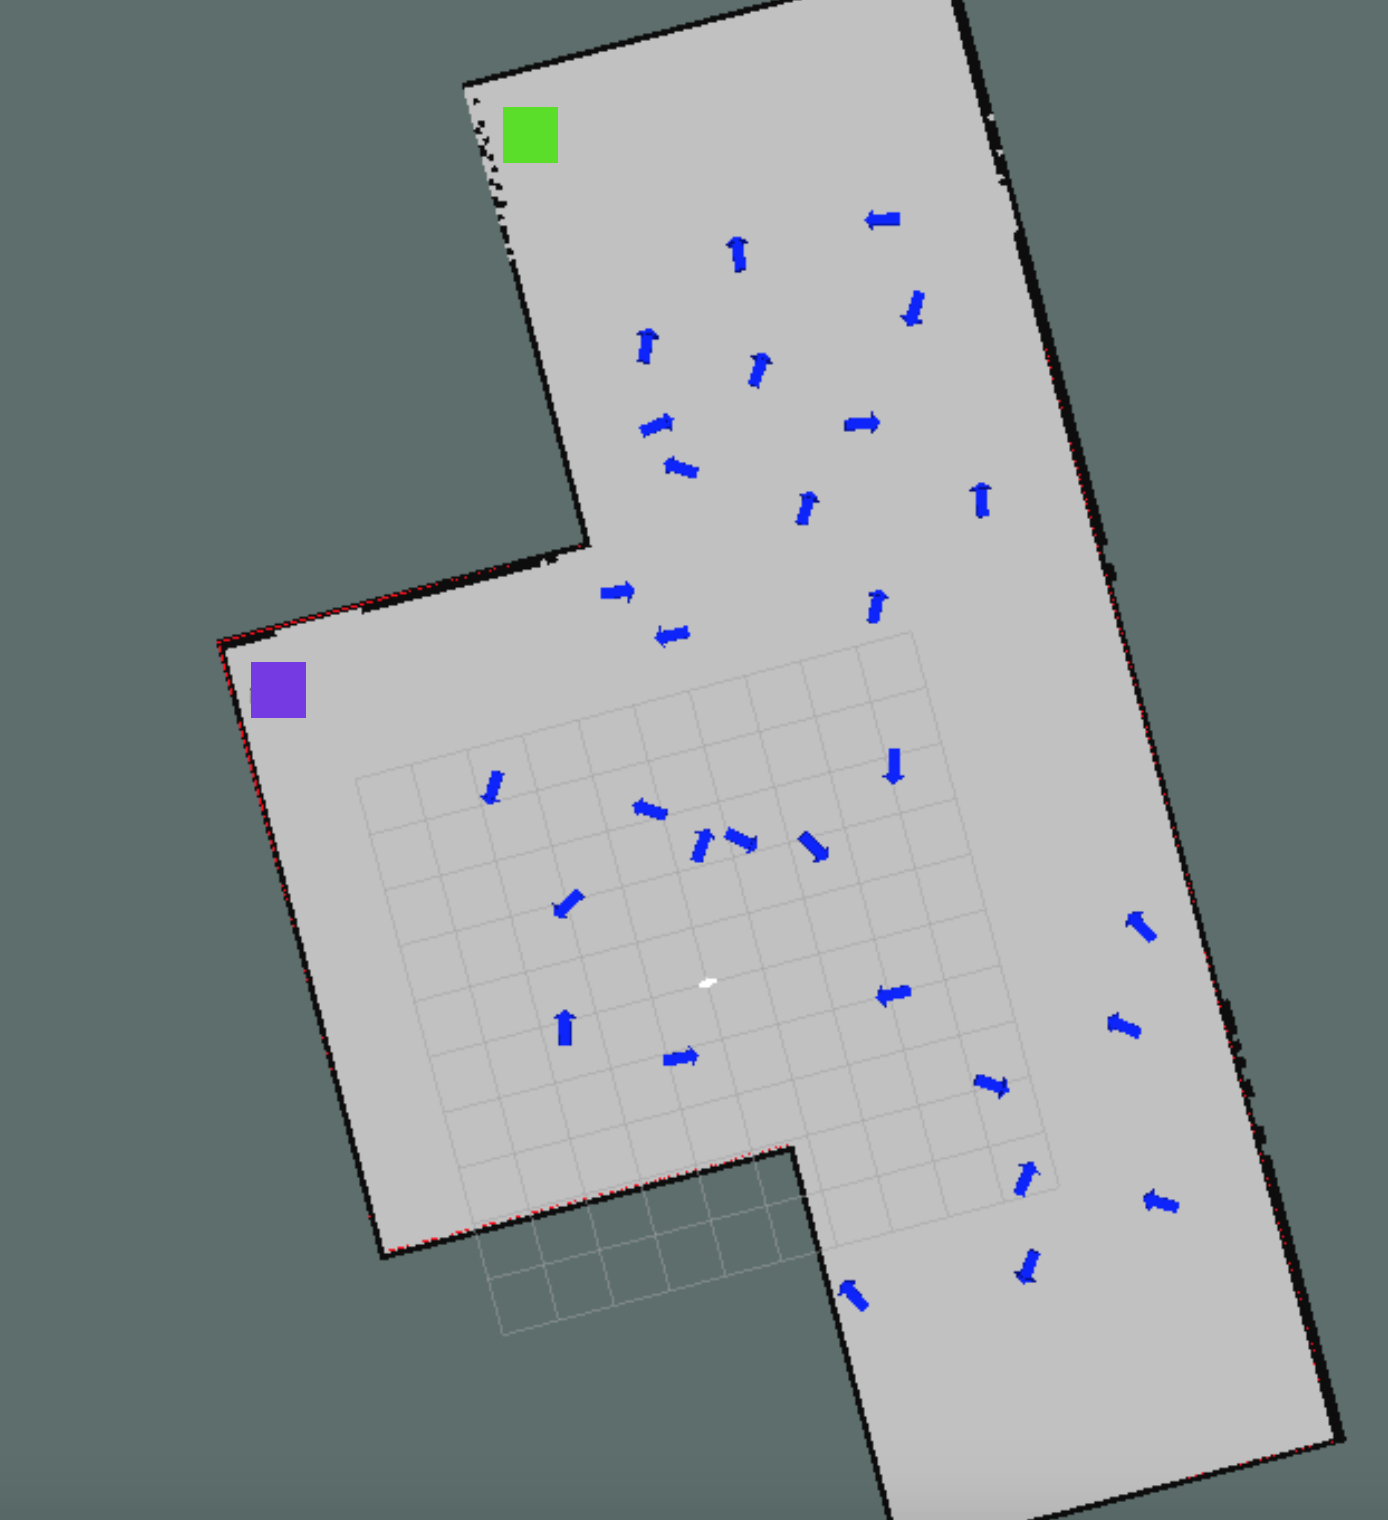
\includegraphics[scale = 0.15]{figures/no_cf.png}
    \caption{Example setting }
    \label{fig:exp_setting}
  \end{subfigure}
  \hspace{10mm}
  \begin{subfigure}[b]{0.35\columnwidth}
  \hspace{4mm}
    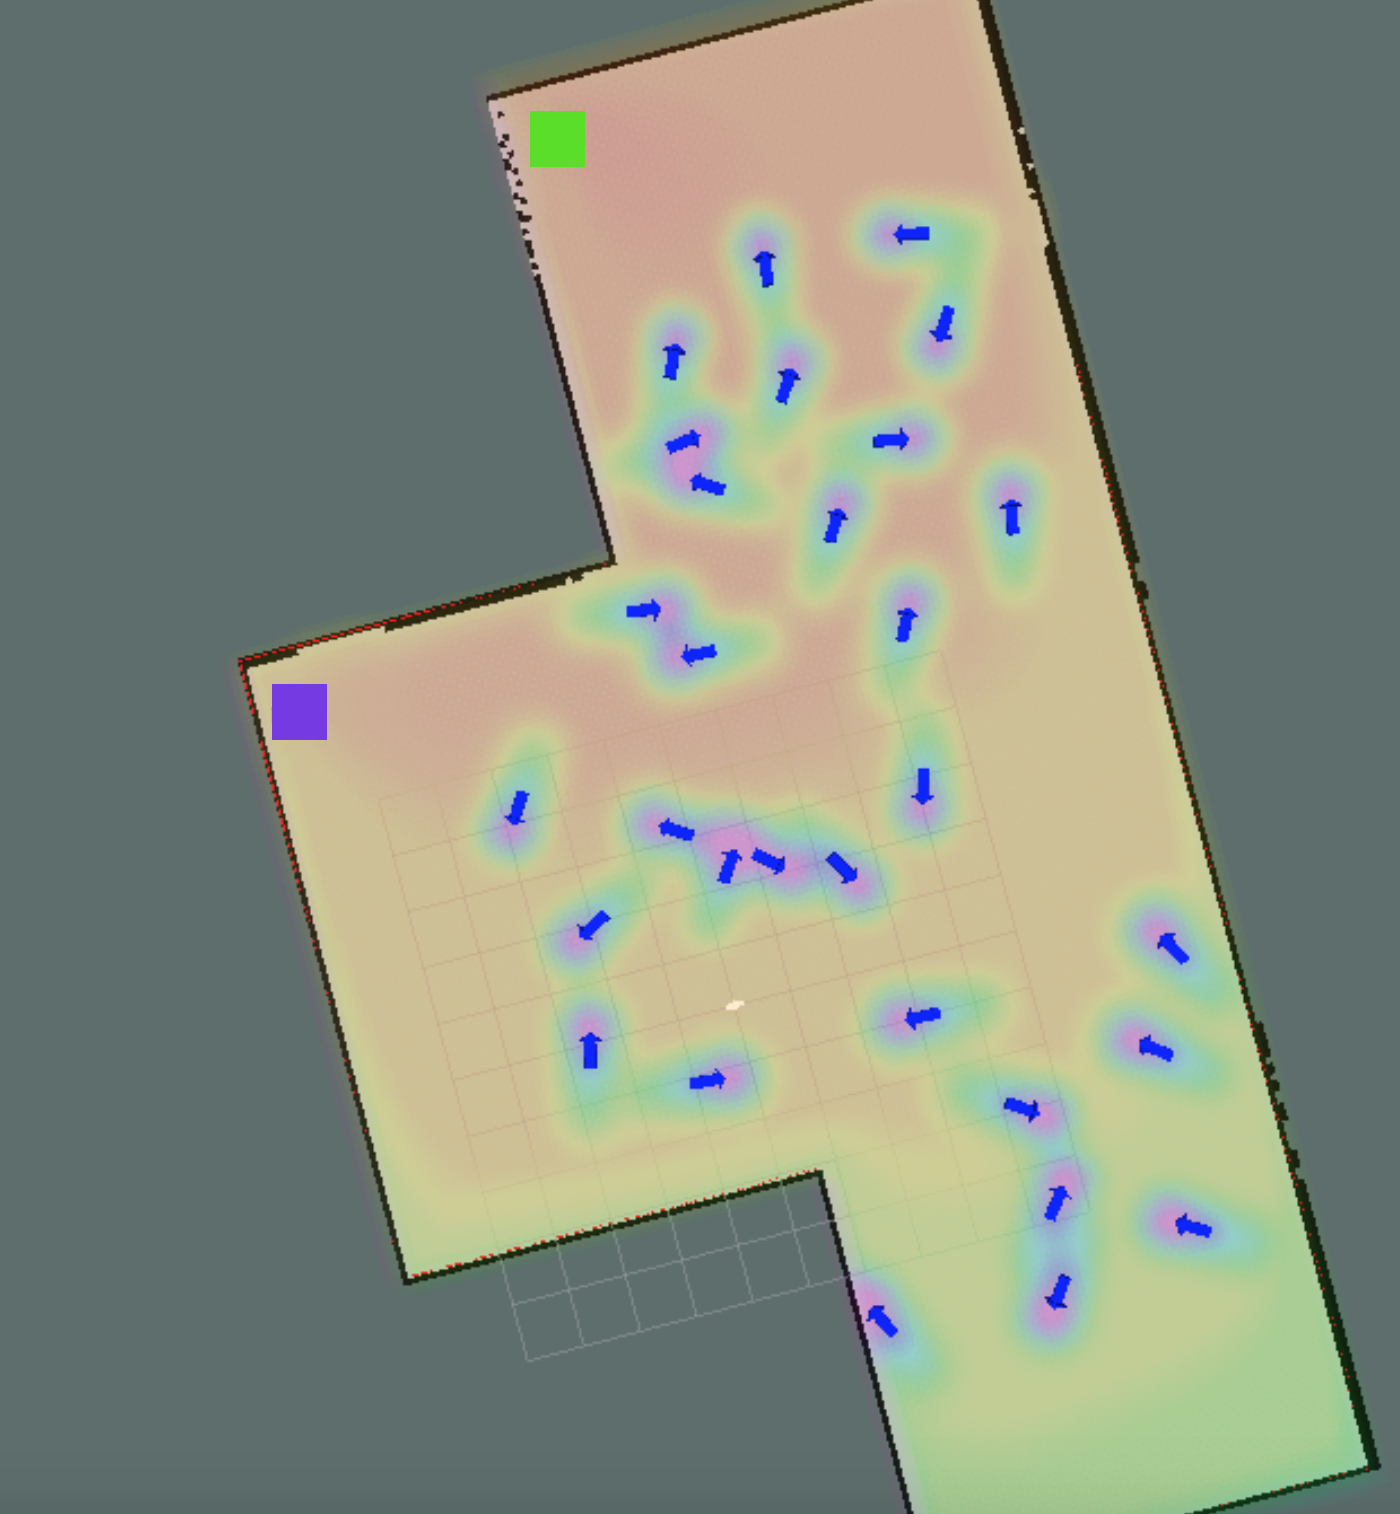
\includegraphics[scale = 0.15]{figures/cf.png}
    \caption{Cost function}
    \label{fig:cost_f}
  \end{subfigure} 

  %\vspace{-3mm}
  \caption{(a) A randomised instance of the social navigation task. Arrows denote the position and orientation of people in the scene. The robot is represented by the magenta box and the goal location is represented by the green box. (b) The corresponding cost function. Red denotes \emph{low} cost, while purple denotes \emph{high} cost.}

    \vspace{-2mm}

  %\vspace{-3mm}
  \label{fig:setting}
  \end{figure}

	The features we use can be divided into three categories. The first category encodes proxemics to the people present in the scene, i.e., the social features. Within this category we consider two variations, for reasons explained in the following section.
	\begin{itemize}
		\item {\bf Social feature set 1 (S1)}: Three isotropic Gaussian functions with different means, centred in front, behind, and on the person.
		\item {\bf Social feature set 2 (S2)}: Three field-of-view features. The features have a value of 1 if the robot is within a certain distance and angle from the person.
	\end{itemize}
	  The second category of features encodes the distance from the target location using linear, exponential, and logarithmic functions. The third category encodes the obstacle cost using a stable function of the reciprocal of the distance from the nearest obstacle. Figure \ref{fig:cost_f} shows an example cost function over the whole configuration space for the configuration in Figure \ref{fig:exp_setting}. We use different functions for human and target proximity, to allow for more degrees of freedom when modelling the underlying cost function. Sufficient regularisation ensures that that the model does not overfit.



% 	\begin{figure}[tbh]
% %	\hspace{-5cm}
% 	\centering
%       \begin{subfigure}[b]{0.42\columnwidth}
%     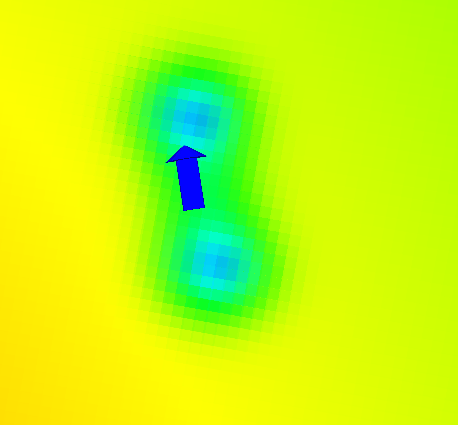
\includegraphics[scale=0.2]{images/person_feat2.png}
%     \caption{Social feature set S1.}
%     \label{fig:S1}
%   \end{subfigure}
%   \hspace{10mm}
%   \begin{subfigure}[b]{0.42\columnwidth}
%   \hspace{4mm}
%     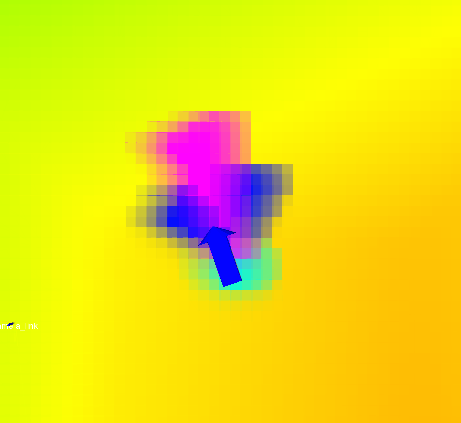
\includegraphics[scale=0.2]{images/person_feat1.png}
%     \caption{Social feature set S2}
%     \label{fig:S2}
%   \end{subfigure} 
%   %\vspace{-3mm}
%   \caption{Cost functions resulting from linear combinations of the social featuresets. Figure \ref{fig:S1} demonstrates featureset 1. It consists of three isotropic Gaussian functions centered in front in the center and behind the person. Figure \ref{fig:S2} shows the field-of-view features of featureset S2. \sw{I have no idea what these plots are showing.} \ks{Now?}}
%     \vspace{-2mm}
%   %\vspace{-3mm}
%   \label{fig:setting}
%   \end{figure}


	\subsubsection{Evaluation}

	To evaluate our algorithms, we generate a dataset $D$ by planning near-optimal paths from initial configurations $s_o$ to goal configurations $s_g$ under a ground-truth cost function $c_{gt}()$ derived from ground-truth weights $\mathbf{w}_{gt}$ and features $\mathbf{F}_{gt}$. A fully optimal path can only be derived asymptotically in terms of either time  for RRT$^*$, or resolution for A$^*$. In practice, however, we found that planning for 100 seconds using  RRT$^*$  achieves a path that is nearly optimal; running longer leads to negligible changes in path cost. 
	The resulting ground truth dataset enables a quantatitive empirical evaluation, which is otherwise problematic in IRL \cite{vasquez2014inverse,shiarlis2016inverse}. For each path $\zeta$ generated by the learning algorithm, we know its cost under the ground-truth cost function and features is simply  $\mathbf{w}_{gt}^T\mathbf{F}_{gt}(\zeta)$. Furthermore, we can compute the \emph{cost difference} between the learned path and the demonstrated path with respect to ground truth:
	\begin{equation}
		Q(\zeta,\zeta_i,\mathbf{w}_{gt}) = \mathbf{w}_{gt}^T(\mathbf{F}_{gt}(\zeta)-\mathbf{F}_{gt}(\zeta_i)), \label{eq:obj_eval}
	\end{equation}
which is our primary performance metric.  Note that, if the demonstration path $\zeta_i$ is optimal under $\mathbf{w}_{gt}$, then $Q(\zeta,\zeta_i,\mathbf{w}_{gt}) \geq 0$. For our holonomic simulated experiments, we consider two learning scenarios.
\begin{enumerate}
	\item \textbf{Unknown weights}: only $\mathbf{w}_{gt}$ is unknown. The demonstrations and the learning algorithm share social feature set S1.
	\item \textbf{Unknown weights and features}: $\mathbf{w}_{gt}$ and $\mathbf{F}_{gt}$  are unknown. S2 is used to generate the demonstrations and S1 is used for learning.
\end{enumerate}

The first scenario evaluates each algorithm's ability to learn good cost functions when provided only with limited demonstrations of the task. The second scenario introduces a feature discrepancy to better simulate real-world settings, since it is unlikely that the features we define will exactly match those implicitly used by the human demonstrator.
% In both cases the ground-truth weights $\mathbf{w}_{gt}$ were chosen to induce a cost function that penalises passing in front of people. In addition, small weights were added to the person related features, as well as linear and exponential penalisation of the distance from the goal, so that the cost functions would not be too trivial. 

We also document the total learning time for K iterations for the algorithms under comparison.  All algorithms were implemented in Python, share similar functions, and were not optimised for speed apart from the caching scheme in RLT$^*$. Finally, we perform a qualitative evaluation by visually comparing the learned cost functions for each algorithm and the paths they generate against ground truth.

	\subsubsection{Holonomic Robot Results}

	Our dataset $D$ consists of 20 trajectories from random social social situations. We split $D$ into $D_{train}$ and $D_{test}$, each with 10 trajectories. After training on $D_{train}$, the cost difference of a cost function is evaluated on $D_{test}$ using \eqref{eq:obj_eval}. The process is repeated 7 times for the same dataset but with different random compositions of $D_{train}$ and $D_{test}$.  All learning algorithms are initialised using the same cost function that only favours shortest paths.
	
	As mentioned earlier, planning time and grid resolution affect the performance of RRT$^*$ and $A^*$, respectively. To make a fair comparison, we vary these two quantities for each algorithm and plot cost difference against learning time at each setting.  We can then identify which algorithms at which settings comprise the Pareto front, i.e., are undominated with respect to cost difference and learning time.
	
	 Figures \ref{fig:res_sim1} and \ref{fig:res_sim2} show the results for the two scenarios described earlier. MMP\_X (green) refers to MMP with X meters of grid resolution while  RLT\_X (red) and RLT$^*$-NC\_X (blue) refer to RLT and RLT without caching, respectively, with X seconds of planning. The shading represents an interpolation of the performance between settings for each method. In this way an area of single colour illustrates hypothesized domination of that method over another, given the same amount of time. Since lower is better for both cost difference and learning time, the closer a point is to the bottom left corner, the better.

	\begin{figure}[tbh]
	\centering
	\captionsetup[subfigure]{justification=centering}
	\hspace{-1cm}
      \begin{subfigure}[b]{0.41\columnwidth}
    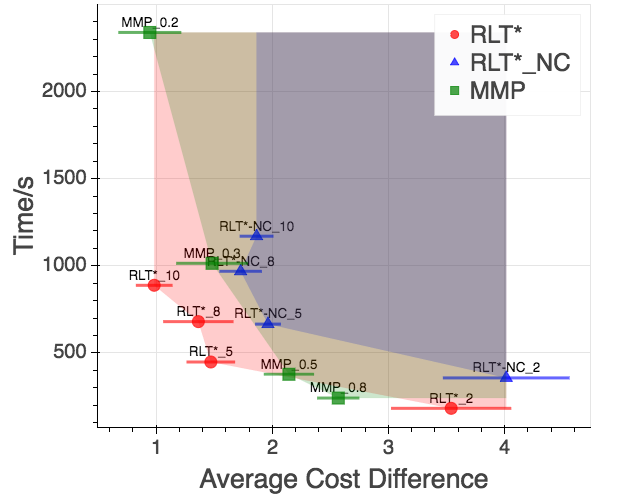
\includegraphics[scale=0.21]{figures/pf_same.png}
    \caption{Unknown weights scenario.}
    \label{fig:res_sim1}
  \end{subfigure}
     	\hspace{10mm}
  \begin{subfigure}[b]{0.41\columnwidth}

    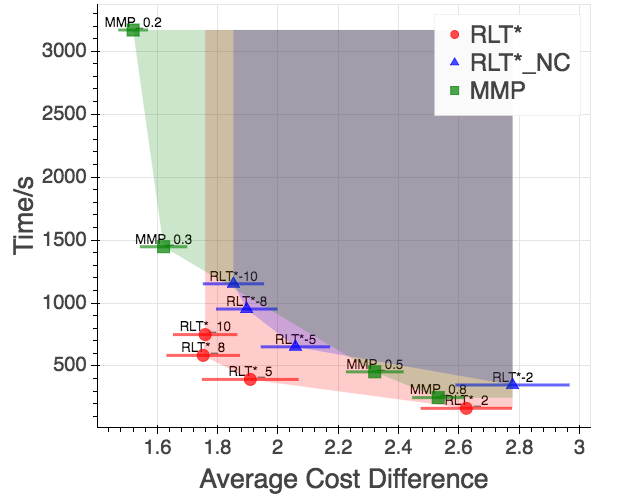
\includegraphics[scale=0.21]{figures/pf_different.png}
    \caption{Unknown weights and features scenario.}
    \label{fig:res_sim2}
  \end{subfigure} 
    \caption{Learning time vs.\ cost difference on the holonomic robot for MMP (green), RLT$^*$-NC (blue), and RLT (red) at different planning fidelities. On both axes \emph{lower is better}.}
    \vspace{-2mm}
  %\vspace{-3mm}
  \label{fig:results_sim}
  \end{figure}

 RLT$^*$ (red) comprises a large majority of the Pareto front, demonstrating good performance and generalisation in reasonable time.  However, the performance of RLT$^*$ and RLT$^*$-NC significantly degrades at very low planning times (2 seconds) because AMMP cannot sample good enough paths to compute a useful gradient.
 
 Note that caching not only speeds learning in RLT$^*$, it also modestly reduces cost differences. This suggests that the caching scheme introduces extra robustness and generalisation capabilities within the algorithm.  As mentioned in Section \ref{subsec:cached}, we hypothesise that the caching scheme improves learning by making the gradients smoother and more consistent, as with momentum. To confirm this, we plot the inner product between successive gradients during learning in Figure \ref{fig:in_prod_grad}. The plot confirms that subsequent gradients in RLT$^*$ are more similar.
 
 Finally, note that MMP's learning time scales exponentially with the size of the grid. This, however, is not solely due to the graph getting larger but also because A$^*$ search scales poorly with the complexity of the cost function itself. Since it relies on an admissible heuristic that for complex cost functions is no longer tight, A$^*$ must expand many more states.  RLT$^*$ is less susceptible to such problems.

 	\begin{figure}[tbh]
%	\hspace{-5cm}
	\centering
    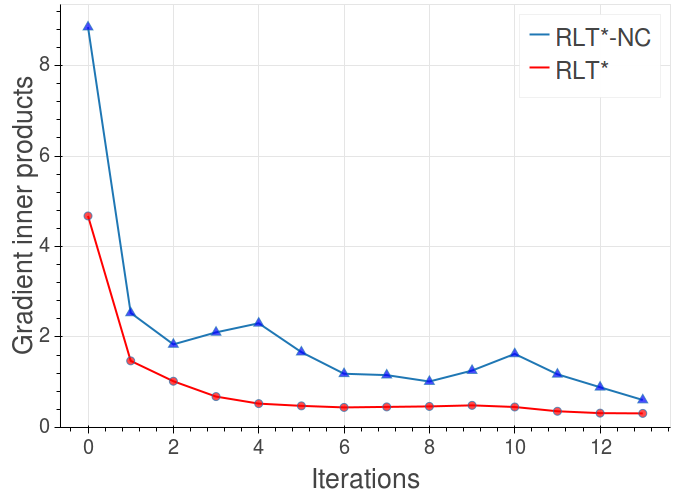
\includegraphics[scale=0.21]{figures/momentum.png}
    \caption{Inner product of succcessive gradients during learning. The smoother curve for RLT$^*$ suggests that fixing the sampled points during learning makes the gradients more consistent. }
    \vspace{-2mm}
  %\vspace{-3mm}
  \label{fig:in_prod_grad}
  \end{figure}


  \subsubsection{Non-Holonomic Robot Results}
  As mentioned earlier, a potential advantage of RLT$^*$ is that it can efficiently handle learning in the presence of motion constraints. In this section, we consider a robot planning in a three-dimensional space, $(x,y,\theta)$, representing the position and orientation of the robot. The robot's motion is further subject to the following motion constraints:
%
  \begin{align}
  	&\dot{x} = v\times\cos(\theta),\\
  	&\dot{y} = v\times\sin(\theta),\\
  	&\dot{\theta} = \omega,
  \end{align}
  where $v,\omega$ are the linear and angular velocities respectively.
  To meet these constraints, we use the POSQ $\texttt{Steer}$ function \cite{palmieri2014novel}.  Since this approach gives a local closed-loop policy between two vertices of the tree, it is  more robust to noise and uncertainty in the motion than an open loop trajectory. Furthermore, it has been shown to produce smooth paths between feasible configurations \cite{palmieri2014novel}. Evaluation is done in the same way as in the previous section, except that we compare RLT$^*$ only to RLT$^*$-NC and not MMP, as the latter cannot handle motion constraints.
RLT$^*$-NC was given 100 seconds to plan, in which case about 3000 configurations were sampled, and RLT$^*$'s cache was set to this size. 

Figure \ref{fig:results_kino} shows that RLT$^*$ is an order of magnitude faster than RLT$^*$-NC, while achieving a lower cost difference. The kinematic constraints contribute to this speedup since they make the \texttt{Steer} and \texttt{Safe} procedures, which are cached, more expensive. As in the holonomic case, RLT$^*$ resulted in smoother learning, confirming the results of Figure \ref{fig:in_prod_grad}. 

  	\begin{figure}[tbh]
	\centering
	\captionsetup[subfigure]{justification=centering}
	\hspace{-1cm}
      % \begin{subfigure}[b]{0.42\columnwidth}
    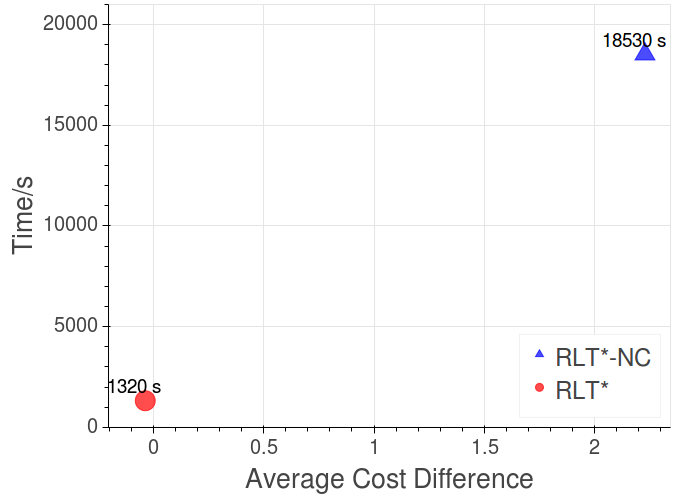
\includegraphics[scale=0.2]{figures/pareto_front_kino.png}
    % \caption{Learning time vs.\ cost difference.}
    % \label{fig:res_kino1}
  % \end{subfigure}
     	% \hspace{10mm}
  % \begin{subfigure}[b]{0.42\columnwidth}

  %   \includegraphics[scale=0.25]{images/cost_diff_val_kino.png}
  %   \caption{Learning curve}
  %   \label{fig:res_kino2}
  % \end{subfigure} 
    \caption{Non-holonomic robot results.}
    \vspace{-2mm}
  %\vspace{-3mm}
  \label{fig:results_kino}
  \end{figure}

Figure \ref{fig:results_qual} shows an instance of the types of paths generated by our method when compared to ground truth. This specific example was drawn from the validation set and is thus not a case of overfitting.


	\begin{figure}[tbh]
%	\hspace{-5cm}
	\centering
    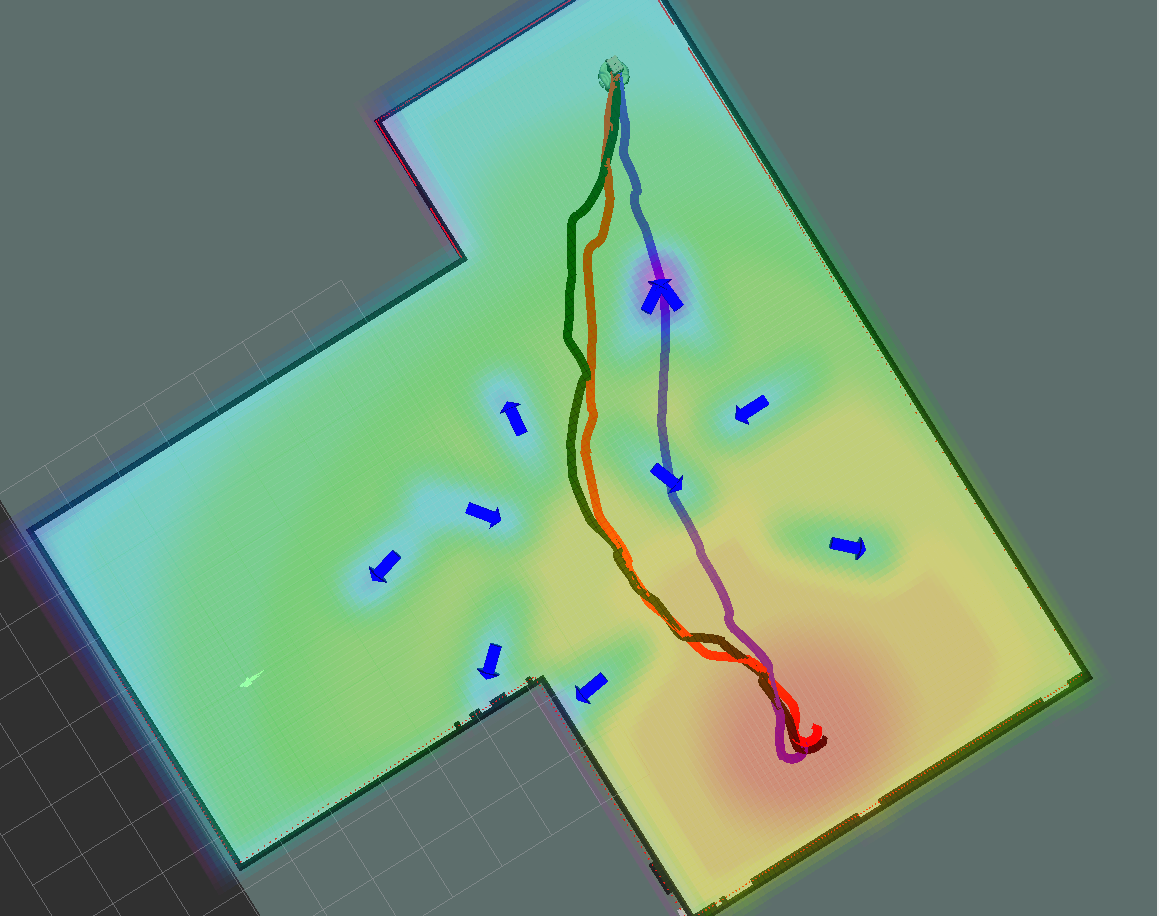
\includegraphics[scale=0.12]{figures/kino_paths.png}
    \caption{Qualitative evaluation of simulated results. The colour map denotes the learned cost function. Red denotes \emph(low) cost and green \emph{high} cost. The learned path (red) is quite similar to the demonstrated path (black) with a clear improvement over the path before learning (purple).}
    \vspace{-2mm}
  %\vspace{-3mm}
  \label{fig:results_qual}
  \end{figure}

	\subsubsection{Real Robot Experiments}
	In this section, we apply RLT$^*$ to real, human demonstrations using a telepresence robot, shown in Figure \ref{fig:robot}, in a social navigation scenario. Furthermore, we deploy the learned cost function on the actual robot.

  	\begin{figure}[tbh]
	\centering
	\captionsetup[subfigure]{justification=centering}
	\hspace{-1cm}
      % \begin{subfigure}[b]{0.42\columnwidth}
    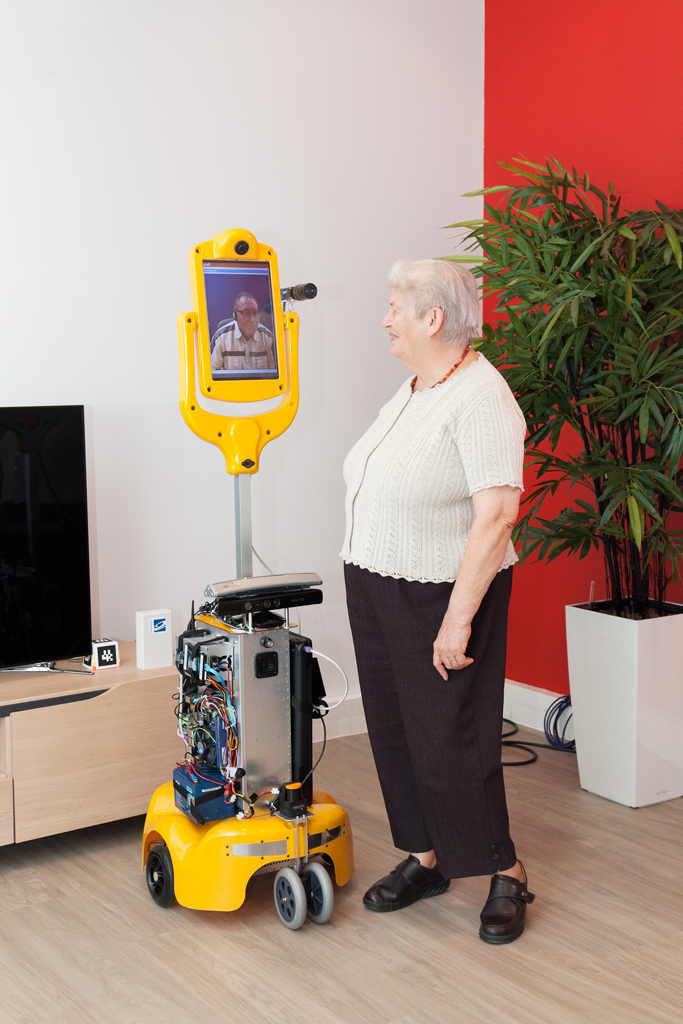
\includegraphics[scale=0.13]{figures/robot.jpg}
    % \caption{Learning time vs.\ cost difference.}
    % \label{fig:res_kino1}
  % \end{subfigure}
     	% \hspace{10mm}
  % \begin{subfigure}[b]{0.42\columnwidth}

  %   \includegraphics[scale=0.25]{figures/cost_diff_val_kino.png}
  %   \caption{Learning curve}
  %   \label{fig:res_kino2}
  % \end{subfigure} 
    \caption{The telepresence robot used in our experiments.}
    \vspace{-2mm}
  %\vspace{-3mm}
  \label{fig:robot}
  \end{figure}

	The experiments take place in a simplified version of the social scenarios we have seen in the previous section. There are two people in the scene at different positions and orientations. A human demonstrator is asked to execute paths for different initial and final conditions across the room. The task is similar to the one used in \cite{okallearning} and the purpose is to find cost functions that account for potential relationships between people depending on their orientation with respect to each other. For example, if people are facing each other, they are  likely engaged in conversation or a similar activity (e.g., taking a photograph) that should not be interrupted. By contrast, if they are looking away from each other and there is enough distance between them then, it might be better to pass between them if doing so yields a shorter path.

	To collect data for learning and validation, we use an off-the-shelf telepresence system augmented with several sensors that allow localisation and perception \cite{shiarlis2015teresa}. We use an Optitrack motion capture system to accurately collect ground truth data of both people and robot positions. RLT$^*$ learns a cost function from this data using the social feature set S1 and the rest of the features described earlier.

Since quantitative evaluation is difficult using real data, as no ground truth is available, we perform a qualitative evaluation instead. Figure \ref{fig:results_real} shows some representative cases that arose during learning. Figure \ref{fig:res_real1} shows a case where RLT$^*$ produced paths (red) that are quite similar to the demonstrated ones (black). Figure \ref{fig:res_real4} shows an instance instances where  the learned paths are reasonable even though they are not similar to the demonstrated paths.

			\begin{figure}[tbh]
%	\hspace{-5cm}
	\centering
      \begin{subfigure}[b]{0.42\columnwidth}
    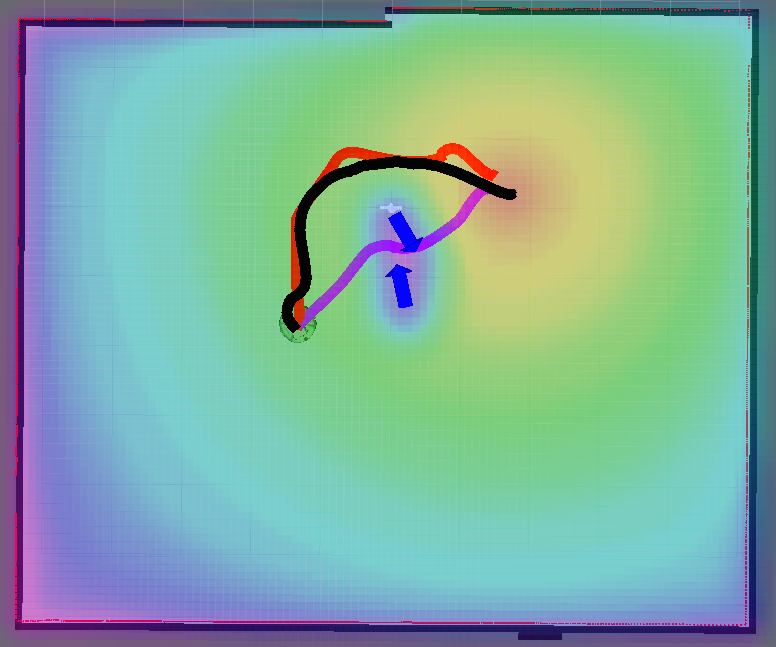
\includegraphics[scale=0.12]{figures/real_good_new.png}
    \caption{}
    \label{fig:res_real1}
  \end{subfigure}
  \hspace{10mm}
  \begin{subfigure}[b]{0.42\columnwidth}
  \hspace{4mm}
    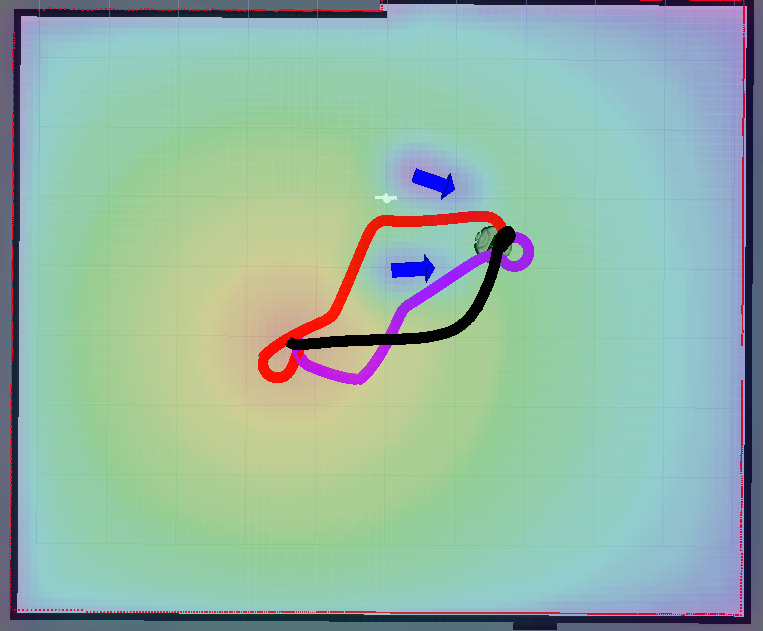
\includegraphics[scale=0.12]{figures/real_reasonable_new.png}
    \caption{}
    \label{fig:res_real4}
  \end{subfigure} 
    \caption{Real demonstrated paths (black), learned paths (red), and shortest paths (purple). In (a), the learned path is similar to the demonstrated path; in (b) it is different but reasonable. The paths are laid over the learned cost function.}
    \vspace{-2mm}
  %\vspace{-3mm}
  \label{fig:results_real}
  \end{figure}


	Finally, we successfully deployed the learned cost function, also shown in Figure \ref{fig:results_real}, on a real telepresence robot. A video demonstrating this deployment can be found in the supplementary material. Even though our planner outputs a full policy in terms of angular and linear velocities, to follow the prescribed path we used an elastic bands local planner in order to deal with dynamic changes in the environment.%\ks{should I say this?} \jm{I think it's ok} 



\vspace{-1mm}
\subsection{Conclusion \& Future Work}
In this paper, we proposed Rapidly Exploring Learning Trees (RLT$^*$), which learns the cost functions of Rapidly Exploring Random Trees (RRT) from demonstration, thereby making inverse learning methods applicable to more complex tasks. Our approach extends the Maximum Margin Planning to work with RRT$^*$ cost functions. Furthermore, it uses a caching scheme that greatly reduces the computational cost and improves performance. Our results in simulated social navigation scenarios show that RLT$^*$ achieves better performance at lower computational cost, even when there is a discrepancy between the features used for demonstration and learning. Furthermore, our results show that RLT$^*$ can handle more complex configuration spaces with motion constraints. Finally, we used RLT$^*$ to learn a cost function using data from real demonstrations on a telepresence robot and successfully deployed that cost function back on the robot.

In future work, we hope to extend RLT$^*$ to model how features evolve over time, in order to, e.g., consider people's movement during planning.  For complex social path planning applications, periodic replanning has been shown to help \cite{henry2010learning,vasquez2014inverse}. Replanning in RRT$^*$ is also possible \cite{otte2015rrtx} and could potentially be incorporated into RLT$*$.
>>>>>>> 3419034cfd28857d99443b62721f4c03cc22e56e


\clearpage





\section{Learning Body Pose Policies from Demonstration}
\label{sec:sl_policy}

Apart from being able to navigate socially, a key functionality for our semi-autonomous telepresence system, is to allow the pilot to engage in conversation 
with the people around the robot, without any input from the pilot himself. While in some ideal conditions this would be a simple tracking problem, (the robot attempts to always face a person), it is no longer the case in real social environments. This is because firstly there could be significant sensor noise, not allowing the robot to track everyone in its surroundings. Secondly, in crowded environments social norms become harder to hard code. For example we might need to converse with various sizes of groups at different formations. The TERESA system attempts to deal with these problems by learning from human interaction.

In Deliverable 5.3 we described in detail, several experiments of people and groups interacting with the robot. During these interactions both the pilot and the interaction target(s) gave direct feedback on the robot`s behaviour. After processing the collected data, two cost functions were produced that allowed us to encode people's prefferences with respect to the robot. In this deliverable we take a different approach. Instead of asking direct feedback from users we employ a human expert to demonstrate the correct behaviour to the robot. Using the collected demonstrations we learn a direct mapping from sensor readings to socially appropriate actions. The rest of the section is organised as follows. 

\begin{itemize}
	\item In Section \ref{sec:demonstration_experiment} we describe local experiments performed at the UvA. The aim of this experiments where to simulate different social situations and extract human demonstrations of control during robot conversation. We further describe how this data was filtered, processed. Finally we describe the input and output representations used in the learning.
	\item In Section \ref{sec:dnn_arch} we describe the use a Deep Neural Network architecture to learn a robust social conversation policy from the collected data, using the data and representations from the previous section. 
	\item Finally in Section \ref{sec:sl_res} we perform an evaluation of our resulting system.
\end{itemize} 

\subsection{Local Experiments and demonstration collection}
\label{sec:demonstration_experiment}
The fist step to achieving the goals set out in this section was to perform experiments in order to collect appropriate demonstration data in various social interaction situations. These experiments took place at the University of Amsterdam in August 2016. These were focused on collecting control data from human demonstrations at different social situations as well as data from all of the robot's sensors. Using machine learning, the aim was to match sequences of input data to the appropriate controls allowing the robot to thus mimic the human demonstrations in new unseen situations. The main aims of the experimental setup and procedure were:

\begin{itemize}
\item To collect data of the robot interacting with various groups sizes.
\item To impose siginificant variability in the sensor and demonstration data 
\end{itemize}

\subsubsection{Experimental Setup}
The setup of this experiment is similar to the one used in the previous deliverable and is depicted in Figure \ref{fig:experiment} . The TERESA robot is placed along with four interaction targets into the "interaction room". Three of the interaction targets are volunteers and vary with each experimental session while one is a researcher from the project. During the experimental session the interaction targets interact with the robot in a social manner. 

The researcher also participates in the interaction but has the additional role of inducing different social situations such that sufficient variability in the data is ensured. This was done by instructing the volunteers to:

\begin{itemize}
 	\item Leave or join the group.
 	\item Sit down or stand up.
 	\item Move
 	\item Change group formation.
\end{itemize}
 Meanwhile in the "control room" another researcher acts as an expert demonstrator, controling the TERESA robot and making sure that the interaction is socially appropriate. 

The following was collected during our experiments:

\begin{itemize}
	\item Linear and angular velocity ($v,\omega$) commands, generated by the expert. 
	\item Person positions  ($x,y$) as detected by the robot's on board localisation module.
	\item Ground truth person positions ($x_{gt},y_{gt}$) using the Optitrack overhead tracking system.
	\item Laser and RGBD sensor data.
	\item Odometry.
\end{itemize}

	\begin{figure}
	\centering
	%\vspace{-3.3mm}
	    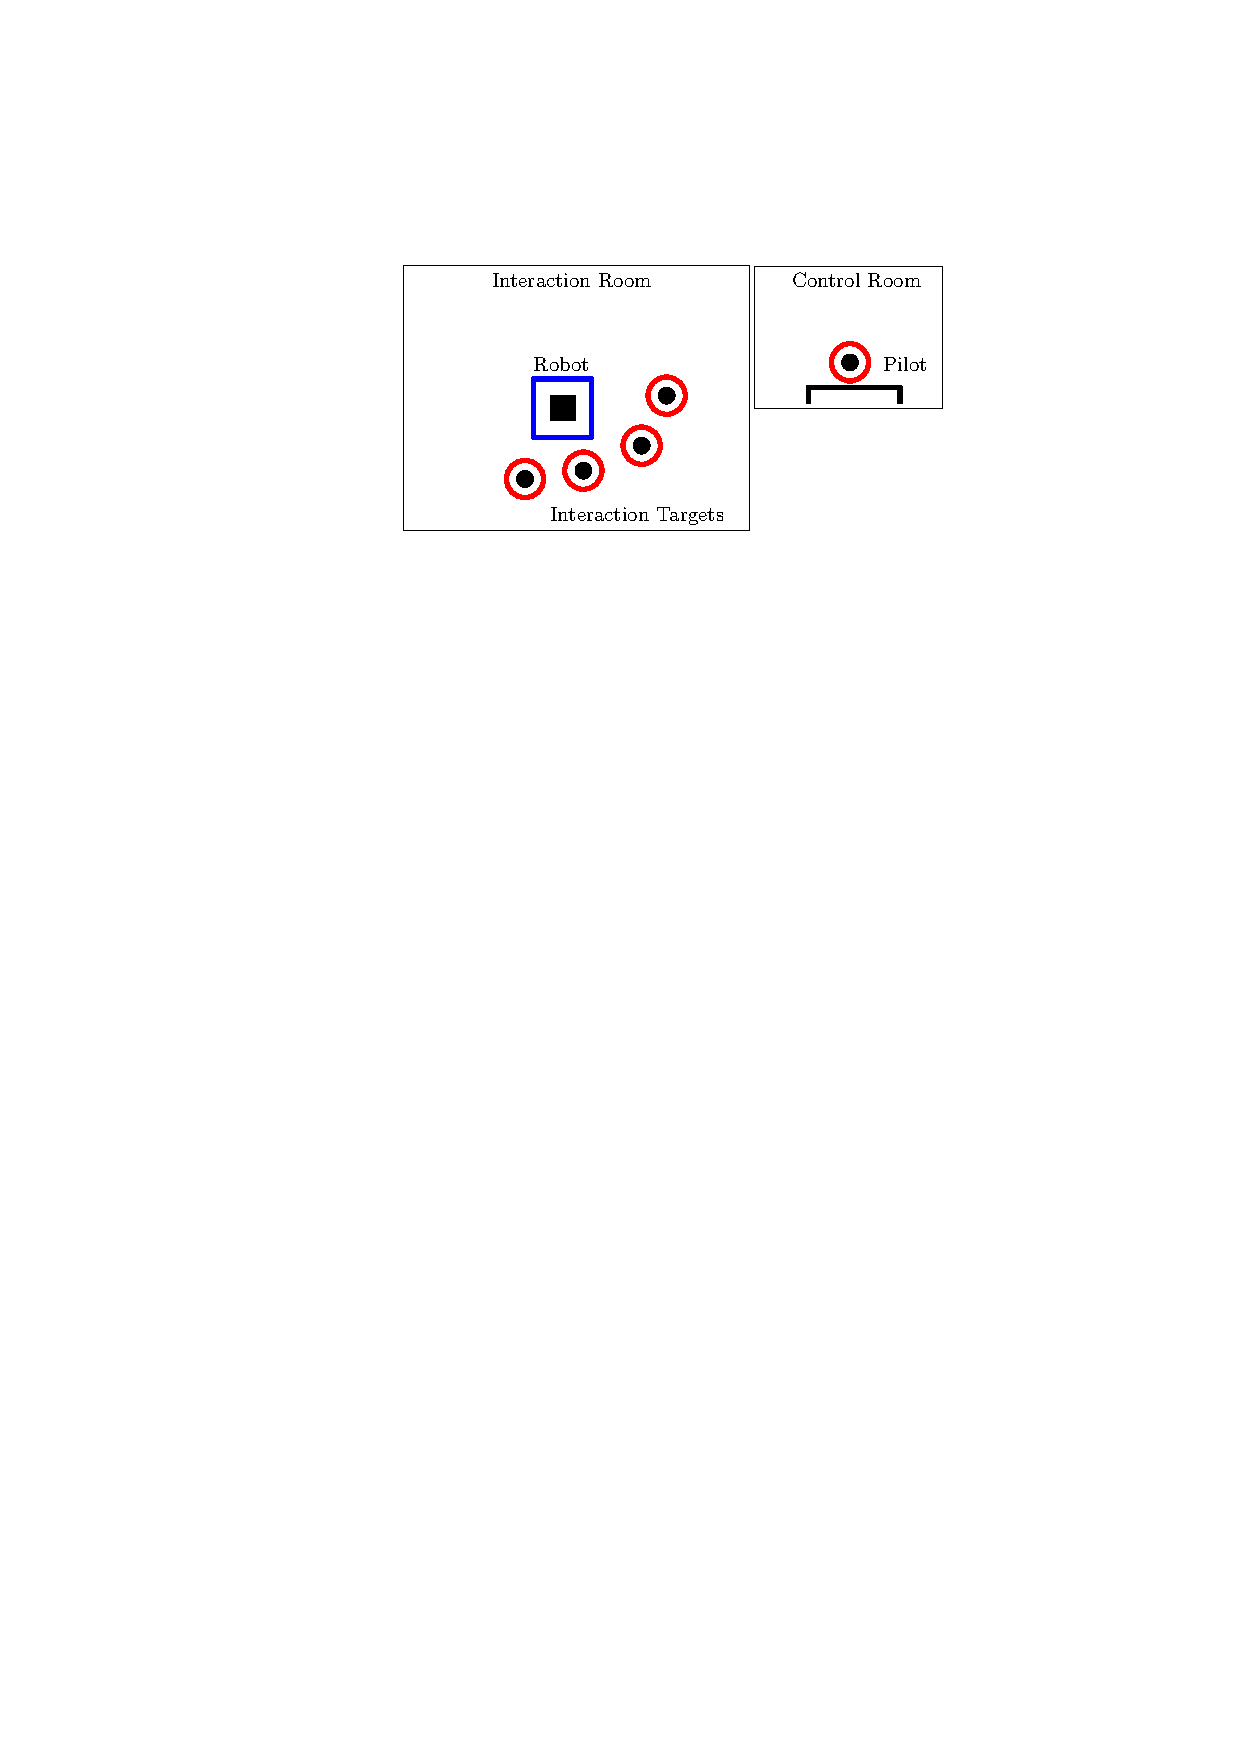
\includegraphics[width=0.8\textwidth]{figures/experiment.pdf}
	%\vspace{-4mm}
	  \caption[Experimental Setting]{The experimental setting}
	  \label{fig:experiment}
	\end{figure}

\subsubsection{Processing}

Before using a learning algorithm to learn a mapping from sensor observations to linear and angular velocities, the collected data was first filtered and processed into an appropriate representation. 

The first step in processing was removing parts where we would not expect the robot to learn a correct mapping for. This occured for example in cases where the participants would quickly move away from the robot, in cases where unusual circumstances took place, or times when the human expert would make an obvious mistake. This data filtering took place by playing back the data and annotating frames where innapropriate data was present, so that they could be ingored further down the pipeline. 

Next using the ground truth data from the Optitrack system we labeled which person was considered to be the interaction target during the conversation. This step is essential because during normal use of the TERESA system an interaction target also needs to be defined by the pilot. The ground truth positions of the interaction targets was not used to correct the readings from the robots localisation system. This ensured that during learning we also learn a model of the localisation system`s noise. 

After filteting the next step was data synchronisation. During the experiments the data from the localisation system and control come at different rates and are thus asynchronous. We synchronised the data by first setting the desired control rate for the final system at 10Hz and then retrieving the latest data from the localisation system and the control outputs at that rate.   

At this point out data consisted of:
\begin{itemize}
	\item Inputs: N Tracked person positions at time t, $\{[x_1,y_1],[x_2,y_2] .., [x_N,y_N]\}_t$.
	\item Outputs: Angular and linear velocity at time t, $\{v,w\}_t$.
\end{itemize}

A naive approach to the problem would attempt to learn a direct mapping from observations at time $t$ to actions at time $t$. This would have very limited chances of success for many reasons. The observations at a single timestep are not only noisy but also cannot encode context information such as the velocity and acceleration of the tracked persons. It is thus required that we augment the input vector to the learning algorithm with past time $\tau$ time instances. The input vector would thus become a concatenation of all tracked person vectors from time $t- \tau$ to $t$ $\{[x_1,y_1],[x_2,y_2] .., [x_{N_{t-\tau}},y_{N_{t-\tau}}]\}_{t-\tau},.. \{[x_1,y_1],[x_2,y_2] .., [x_{N_t},y_{N_t}]\}_t$ and the output would remain to be angular and linear velocity at time t.

Another problem with our input data is that the number of tracked persons at each time step varies. This variability in the input data makes processing using conventional Machine Learning methods difficult. One way to combat this problem is to set a max number of tracked people at each timestep, $N_{max}$. We would then make sure to include the closest $N_{max}$ tracked persons at each time. If $N_t$ would be less than $N_{max}$ then we could pad that vector with zeros. While this would be a viable option it could pose several difficulties for learning in practice. As an example picture two successive frames with different number of people. Were we to ensure that past frames are constant we would have to make sure that if a person is the same in the two time slots they should be put into the same person slot in order to facilitate learning, this could make data hard to preprocess and still lead to mistakes. For this reason we take a slightly different approach. For each input vector at time t we create an image such as the one shown in Figure \ref{fig:state}. Each person is drawn onto the image as a circle with intensity 1 while the interaction target is drawn as a circle with intensity 2. The position of this circles is determined by the person positions with respect to the robots frame. The created image has a fixed size and resolution which means that it can only represent persons that are present at a maximum distance of $d$ from the robot. In our $d$ was set to 2.5m. 

<<<<<<< HEAD
  	\begin{figure}[tbh]
	\centering
    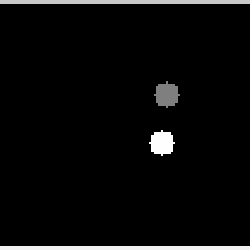
\includegraphics[scale=0.50]{figures/state.png}
    \caption[Image representation of the robot's state]{The Image representation of the robot's state. The bright circle is the interaction target, the grey is another detected person. The robot is facing towards the positive x-axis of the image. Hence in this case the two people are just in front of the robot. }
  \label{fig:state}
=======
  	\begin{figure}[tbh]
	\centering
    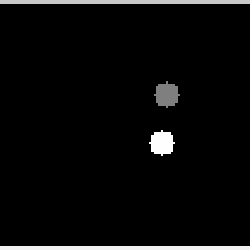
\includegraphics[scale=0.50]{figures/state.png}
    \caption{The Image representation of the robot's state. The bright circle is the interaction target, the grey is another detected person. The robot is facing towards the positive x-axis of the image. Hence in this case the two people are just in front of the robot. }
  \label{fig:state}
>>>>>>> 3419034cfd28857d99443b62721f4c03cc22e56e
  \end{figure}

Another advantage of the image representation is that it allows us to use state of the art machine learning methods that exploit spacial structure in images such as convolutional neural networks which have proved to be very effective in image processing tasks \cite{krizhevsky2012imagenet}. This is explored in the next section.

\subsubsection{Outputs}
The learning algorithm is expected to output a policy, i.e. a control output for a set of inputs. While our outputs are linear and angular velocities, it is not clear wether having continuous or discrete outputs is better in terms of learning and performance of the resulting policy. Having discrete outputs results in a classification problem which is typically easier to solve than a regression problem, which is the case with a continuous representation. Another drawback of continuous representations is that the output distribution could be mutimodal, which is something that continuous output networks do not typically account for. However a continuous representation is much more natural in this case and could result in a much more aggreable behaviour from the robot. For this reason we decided to try both representations and choose best one after deployment on the robot. 

Another problem in terms of the outputs, for this specific application sourced from the fact that during the training data, the robot was stopped for far longer than it was actually moving. This posed problems in both the cases of a continuous and a discrete output. In the discrete case, far more datapoints where in the specific class of $(v,\omega) = (0,0)$ than any of the other individual classes, this can hurt the learning or even urge the network to simply output that class if sufficient measures are not taken. In the continuous case, it may cause the network to output smaller velocities than required. To combat this effect we took two measures. First we made sure that a similar portion of static and moving outputs where present in the data. Secondly we experimented with a hierarchical output architecture. In this case, the learning algorithm must first clasify wether or not the output should be (0,0) or something else. Then given that the output is not (0,0) it decides what the output should be. This feature made a big difference when deployed on the robot and it is hence present in all the models we consider.


\subsection{Learning} \label{sec:dnn_arch}

In the previous section we detailed the form of our input states and output controls for the learning task treating the actual algorithm as a black box. We reasoned that an input image representation such as the one shown in Figure \ref{fig:state} would be more appropriate. We further argued that the learning procedure would be much more effective if the evolution of these images over time was to be taken into account. In this section we use these two key points to construct a deep neural network (DNN) architecture in order to learn this mapping from inputs to controls.

\subsubsection{Convolutional Layers}
Convolutional neural networks have been particuarly effective in extracting useful features from static images \cite{krizhevsky2012imagenet}. Input to a convolutional layer is an $n_i \times n_i$ image with $c_i$ channels. The input convolved by a set of $K$ filters of dimentions $n_f \times n_f$, resulting in $K$ output feature maps. These are then subject to a non-linearity, in this case a rectified linear unit (ReLu) and possibly a subsampling operation, in this case max pooling. The result of the computation can then be considered a new image of $K$ channels and dimention $n_1 \times n_1$, where the subscript denotes the layer number. This procedure may thus be repreated for many layers of computation. A key aspect of convolutional networks is that the filter weights (or shapes) are learned. This means that they can be trained to extact the image features usefull for the specific application. Such a convolutional layer is shown in Figure \ref{fig:conv_layer}.

	\begin{figure}
	\centering
	%\vspace{-3.3mm}
	    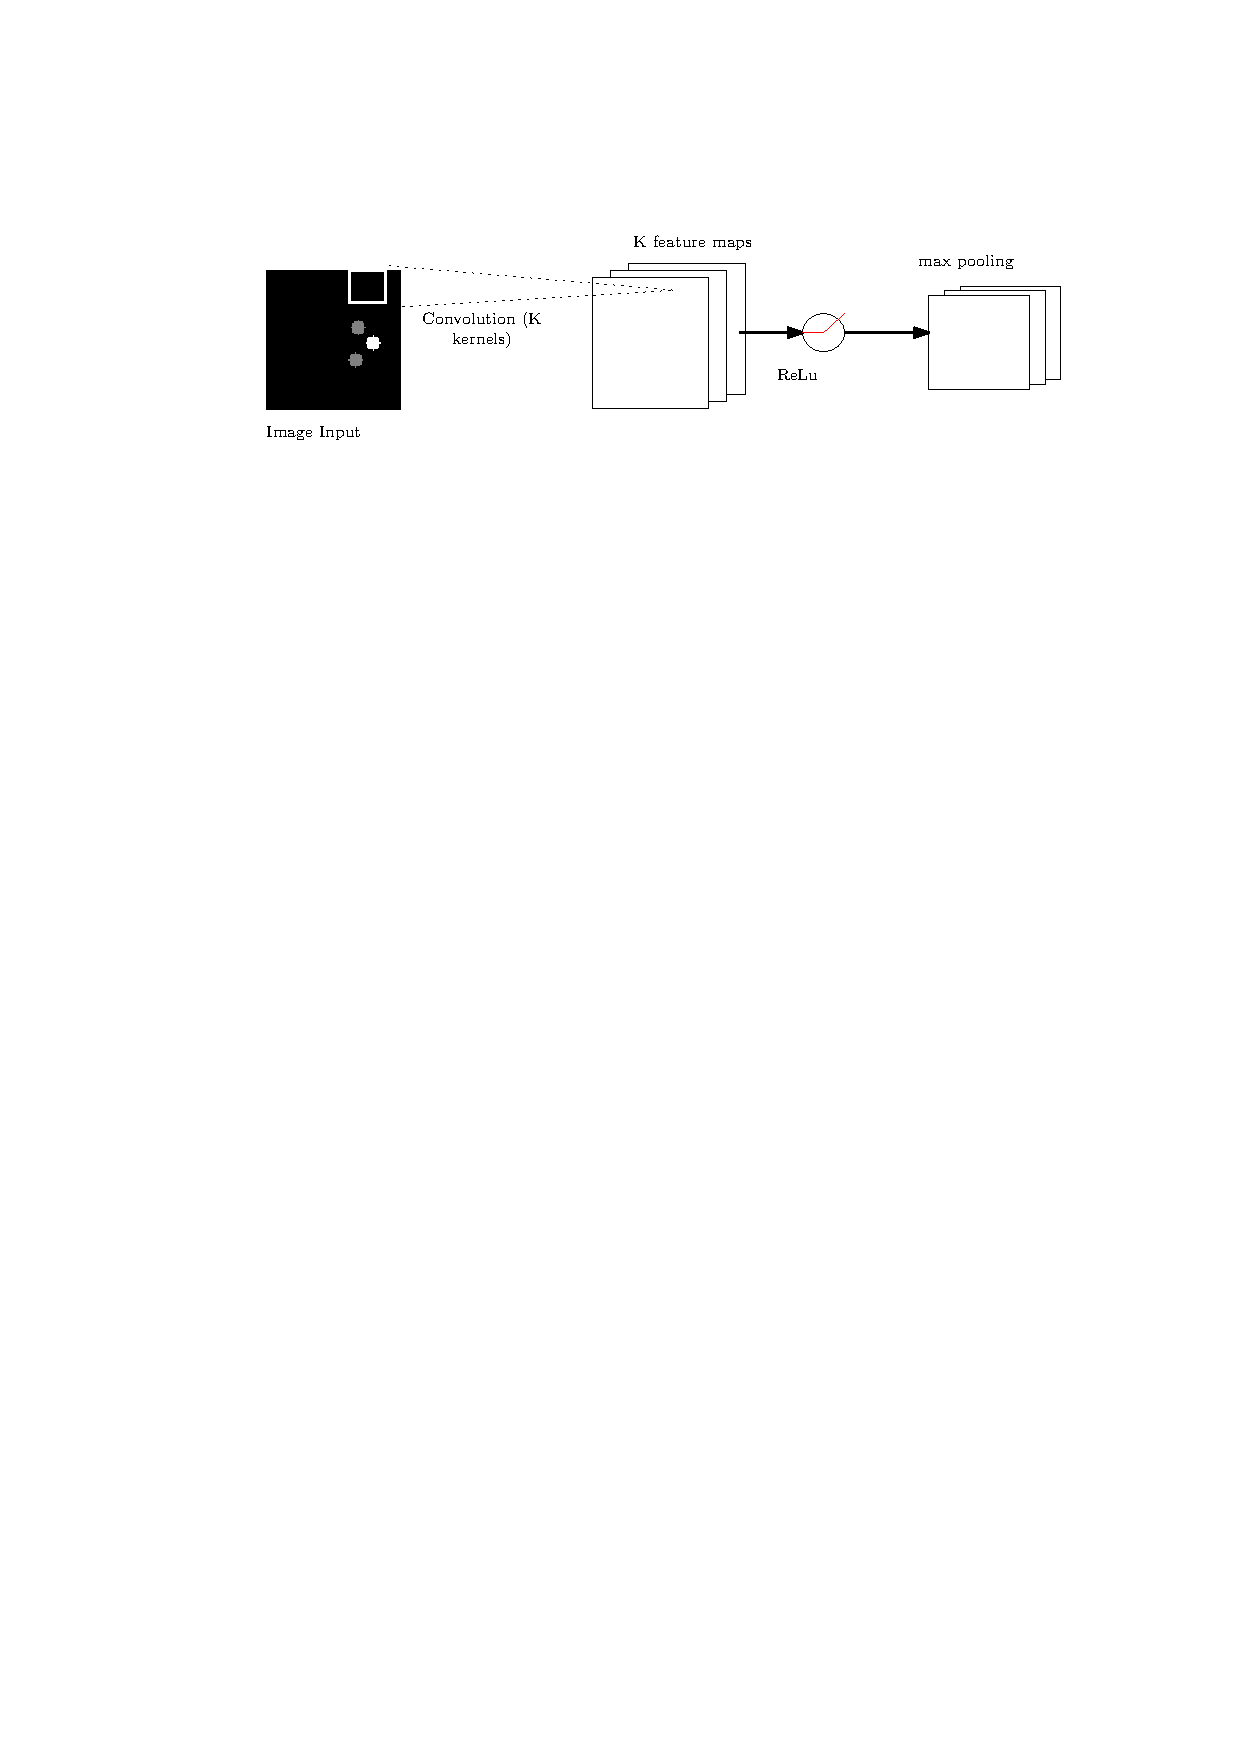
\includegraphics[width=0.8\textwidth]{figures/conv_layer.pdf}
	%\vspace{-4mm}
	  \caption[A convolutional layer]{A convolutional layer.}
	  \label{fig:conv_layer}
	\end{figure}


\subsubsection{Long Short Term Memory}
Recurrent neural network architectures allow DNNs to deal with input sequences instead of simply static inputs.
In contrast to fully connected and convolutional networks, an RNN allows the network to retain a state based on its previous inputs. This is done by essentially feeding back to the network a representation of the previous inuput. This makes them ideal in dealing with time varying and variable length inputs. An outline of an RNN is shown in Figure \ref{fig:RNN}.
\def\layersep{1.5cm}
\begin{figure}[h!]
\centering
\begin{tikzpicture}[shorten >=1pt,->,draw=black!50, node distance=2.5cm]
    \tikzstyle{every pin edge}=[<-,shorten <=1pt]
    \tikzstyle{neuron}=[circle,very thick,minimum size=17pt,inner sep=2pt]
    \tikzstyle{input neuron}=[neuron, draw=black!50, fill=white];
    \tikzstyle{output neuron}=[neuron, draw=black!50, fill=white];
    \tikzstyle{hidden neuron}=[neuron, draw=black!50, fill=white];
    \tikzstyle{annot} = [text width=4em, text centered]

    % Draw the input layer nodes
    \foreach \name / \y in {1,...,3}
    % This is the same as writing \foreach \name / \y in {1/1,2/2,3/3,4/4}
        \node[input neuron] (I-\name) at (0,-\y) {};
        
    \draw [->, thick, >=stealth', bend left=200, looseness=7] (I-2.east) to node [swap] {}  (I-2.west);
    
    \path (I-3) edge (I-2);
    \path (I-2) edge (I-1);    
    
    \node[text width=0cm] (x) at (-0.15, -1.0) {$o_t$};
    \node[text width=0cm] (h) at (-0.15, -2.0) {$h$};
    \node[text width=0cm] (o) at (-0.15, -3.0) {$x_t$};
    
    \node[text width=0cm] (o) at (\layersep-0.15cm, -2.0) {$\Rightarrow$};
    
    % Draw expanded network
    \foreach \name / \x in {1/1,2/2,4/4}
        \foreach \namee / \y in {1,...,3}
            \node[input neuron] (I-\name-\namee) at (\layersep+\layersep*\x,-\y) {};
            
    \path (I-1-3) edge (I-1-2);
    \path (I-1-2) edge (I-1-1);
    \path (I-1-2) edge (I-2-2);
    \path (I-2-3) edge (I-2-2);
    \path (I-2-2) edge (I-2-1);
    \path (I-2-2) edge (I-4-2);
    \path (I-4-3) edge (I-4-2);
    \path (I-4-2) edge (I-4-1); 
    
    \node[text width=0cm] (x) at (\layersep * 2 -0.15cm, -1.0) {$o_0$};
    \node[text width=0cm] (h) at (\layersep * 2 -0.15cm, -2.0) {$h_0$};
    \node[text width=0cm] (o) at (\layersep * 2 -0.15cm, -3.0) {$x_0$};
    \node[text width=0cm] (x) at (\layersep * 3 -0.15cm, -1.0) {$o_1$};
    \node[text width=0cm] (h) at (\layersep * 3 -0.15cm, -2.0) {$h_1$};
    \node[text width=0cm] (o) at (\layersep * 3 -0.15cm, -3.0) {$x_1$};
    \node[text width=0cm] (h) at (\layersep * 4 -0.15cm, -1.0) {$\dots$};
    \node[text width=0cm] (o) at (\layersep * 4 -0.15cm, -3.0) {$\dots$}; 
    \node[text width=0cm] (x) at (\layersep * 5 -0.15cm, -1.0) {$o_t$};
    \node[text width=0cm] (h) at (\layersep * 5 -0.15cm, -2.0) {$h_t$};
    \node[text width=0cm] (o) at (\layersep * 5 -0.15cm, -3.0) {$x_t$}; 
\end{tikzpicture}
\caption{An unfolded recurrent neural network.}
\label{fig:RNN}
\end{figure}
  
Long short term memory networks (LSTM) \cite{hochreiter1997long} are an effective standard architecture for Recurrent Neural Networks. While the general architecture follows the one shown in Figure \ref{fig:RNN}, the way that the feedback and output of the network are computed is especially designed to prevent the gradients during learning from exploding or becoming too small. This has allowed LSTMs to excell in various sequence prediction tasks such as handwriting and speech recognition. 

We have argued in the previous section, that it would be very hard to learn a mapping from inputs to demonstrations if the robot would have no memory of past input states (images). This is because, simply put, the environment is partially observable. Using the LSTMs allows the network to use past inputs, which in turn allows it to disambiguate between different input images and makes it more robust to the person localisation system`s false possitives. 

\tikzstyle{block} = [draw,rectangle,thick,minimum height=2em,minimum width=2em]
\usetikzlibrary{shapes,snakes}
\begin{figure}[h!]
  \hspace{-1cm}
  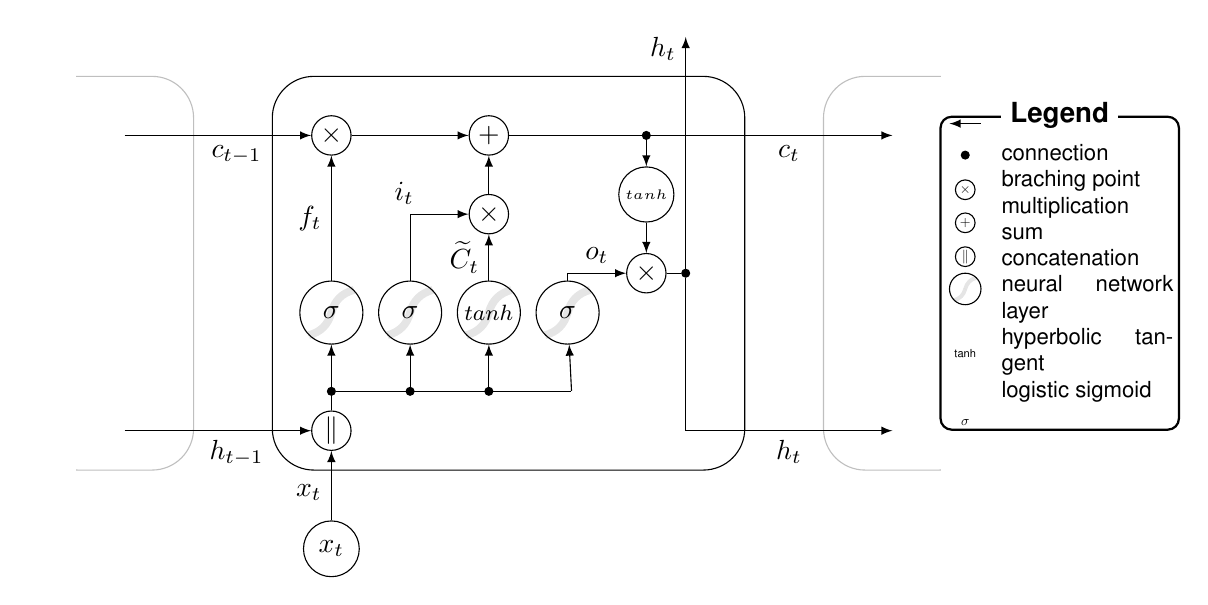
\begin{tikzpicture}
  \draw[rounded corners=15pt, color=lightgray] (-3,0) rectangle (-1,5);
  \draw[fill=white, color=white] (-3.1,-0.1) rectangle (-2.5,5.1);
  \draw[rounded corners=15pt] (0,0) rectangle (6,5);
  \draw[rounded corners=15pt, color=lightgray] (7,0) rectangle (9,5);
  \draw[fill=white, color=white] (8.5,-0.1) rectangle (9.1,5.1);

  \node (Htm1) at (-2,0.5) {};
  \node (Ctm1) at (-2,4.25) {};
  \node (Htm2) at (8,0.5) {};
  \node (Ctm2) at (8,4.25) {};
  
  %\node [rounded corners, draw=black, rectangle split, rectangle split parts=2] (zt) at (1,1.5) {\textbf{$z_t$} \nodepart{second} \footnotesize $(h_{t-1}\Vert x_t)$};
  \node[draw=black,circle, minimum size=0.5cm,inner sep=0pt] (Ct) at (0.75,4.25) {\textbf{$\times$}};
  
    \node[draw=black,circle, minimum size=0.8cm,inner sep=0pt] (sig1) at (0.75, 2) {$\sigma$};
    \draw [-, line width=1mm, bend left=60, bend right=30, looseness=1, opacity=0.1] (sig1.south west) to node [swap] {}  (sig1.center);
    \draw [-, line width=1mm, bend left=0, bend right=-30, looseness=1, opacity=0.1] (sig1.center) to node [swap] {}  (sig1.north east);
    
    \node[draw=black,circle, minimum size=0.8cm,inner sep=0pt] (sig2) at (1.75, 2) {$\sigma$};
    \draw [-, line width=1mm, bend left=60, bend right=30, looseness=1, opacity=0.1] (sig2.south west) to node [swap] {}  (sig2.center);
    \draw [-, line width=1mm, bend left=0, bend right=-30, looseness=1, opacity=0.1] (sig2.center) to node [swap] {}  (sig2.north east);
    
        \node[draw=black,circle, minimum size=0.8cm,inner sep=0pt] (tanh1) at (2.75, 2) {\footnotesize $tanh$};
    \draw [-, line width=1mm, bend left=60, bend right=30, looseness=1, opacity=0.1] (tanh1.south west) to node [swap] {}  (tanh1.center);
    \draw [-, line width=1mm, bend left=0, bend right=-30, looseness=1, opacity=0.1] (tanh1.center) to node [swap] {}  (tanh1.north east);
    
    \node[draw=black,circle, minimum size=0.8cm,inner sep=0pt] (sig3) at (3.75, 2) {$\sigma$};
    \draw [-, line width=1mm, bend left=60, bend right=30, looseness=1, opacity=0.1] (sig3.south west) to node [swap] {}  (sig3.center);
    \draw [-, line width=1mm, bend left=0, bend right=-30, looseness=1, opacity=0.1] (sig3.center) to node [swap] {}  (sig3.north east);
  
    \node[draw=black,circle, minimum size=0.5cm,inner sep=0pt] (zt) at (0.75,0.5) {\textbf{$\Vert$}};
  
    \node[draw=black,circle, minimum size=0.5cm,inner sep=0pt] (Ct2) at (2.75,4.25) {\textbf{$+$}};
   \node[draw=black,circle, minimum size=0.5cm,inner sep=0pt] (Ct3) at (2.75,3.25) {\textbf{$\times$}};  
   
   \node[draw=black,circle, minimum size=0.7cm,inner sep=0pt] (tanh) at (4.75, 3.5) {\tiny $tanh$};
   \node[draw=black,circle, minimum size=0.5cm,inner sep=0pt] (out1) at (4.75,2.5) {\textbf{$\times$}};     
   
  
  \node[draw=black,fill=black,circle, minimum size=0.1cm,inner sep=0pt] (split1) at (0.75,1) {};
  \node[draw=black,fill=black,circle, minimum size=0.1cm,inner sep=0pt] (split2) at (1.75,1) {};
  \node[draw=black,fill=black,circle, minimum size=0.1cm,inner sep=0pt] (split3) at (2.75,1) {};
  \node[draw=black,fill=black,circle, minimum size=0cm,inner sep=0pt] (split4) at (3.8,1) {};
  
  \node[draw=black,fill=black,circle, minimum size=0.1cm,inner sep=0pt] (split5) at (4.75,4.25) {};
  
  \node[draw=black,fill=black,circle, minimum size=0.1cm,inner sep=0pt] (split6) at (5.25,2.5) {};
  
  \draw[-latex] (Htm1) -- (zt) node[pos=0.6, below] {$h_{t-1}$};
  \draw[-latex] (Ctm1) -- (Ct) node[pos=0.6, below] {$c_{t-1}$};
  \draw[-latex] (zt) -- (sig1);% node[pos=0.7, left] {$z_t$};
  \draw[-latex] (split2) -- (sig2);% node[pos=0.5, left] {$z_t$};
  \draw[-latex] (split3) -- (tanh1);%; node[pos=0.5, left] {$z_t$};
  \draw[-latex] (split4) -- (sig3);%; node[pos=0.5, left] {$z_t$};  
  \draw[-latex] (sig1) -- (Ct) node[pos=0.5, left] {$f_t$};
  \draw[-latex] (Ct) -- (Ct2);
  \draw[-latex] (Ct3) -- (Ct2);
  \draw[-latex] (tanh1) -- (Ct3) node[pos=0.5, left] {$\widetilde{C}_t$};
  \draw[-latex] (Ct2) -- (Ctm2) node[pos=0.73, below] {$c_t$};
  \draw(sig2) -- (1.75,3.25);  
  \draw[-latex] (1.75,3.25) -- (Ct3) node[pos=-0.1, above] {$i_t$};
  \draw (split1) -- (split4) ;
  \draw(sig3) -- (3.75,2.5) ;
  \draw[-latex] (3.75,2.5) -- (out1) node[pos=0.5, above] {$o_t$}; 
  \draw[-latex] (split5) -- (tanh);
  \draw[-latex] (tanh) -- (out1);
  \draw(out1) -- (split6);
  \draw[-latex] (split6) -- (5.25,5.5) node[pos=0.95, left] {$h_t$}; 
  \draw (split6) -- (5.25,0.5);
  \draw[-latex] (5.25,0.5) -- (Htm2) node[pos=0.5, below] {$h_t$};
  
  \node[draw=black,circle] (xt) at (0.75, -1) {$x_t$};
  
  \draw[-latex] (xt) -- (zt) node[pos=0.4, left] {$x_t$};

  \tikzstyle{mybox} = [draw=black, thick,
    rectangle, rounded corners, inner sep=2pt, inner ysep=10pt]
    
  \node [mybox] (box) at (10,2.5) {
   \begin{minipage}{0.05\textwidth}\hspace{2em}\end{minipage}
   \begin{minipage}{0.18\textwidth}
      \footnotesize
      connection\\
      braching point\\
      multiplication\\
      sum\\
      concatenation\\
      neural network layer\\
      hyperbolic tangent\\
      logistic sigmoid
   \end{minipage}}; 
  \node[fill=white] at (box.north) {\textbf{Legend}};

  \draw[-latex](9,4.4) -- (8.6,4.4);
  \node[draw=black,fill=black,circle, minimum size=0.1cm,inner sep=0pt] (legend_split) at (8.8,4) {};
   \node[draw=black,circle, minimum size=0.5cm,scale = 0.5,inner sep=0pt] (legend_mult) at (8.8,3.56) {\textbf{$\times$}};
   \node[draw=black,circle, minimum size=0.5cm,scale = 0.5,inner sep=0pt] (legend_plus) at (8.8,3.14) {\textbf{$+$}};
   \node[draw=black,circle, minimum size=0.5cm,scale = 0.5,inner sep=0pt] (legend_vert) at (8.8,2.71) {\textbf{$\Vert$}};
    
    \node[draw=black,circle, minimum size=0.8cm,scale = 0.5, inner sep=0pt] (legend_neural) at (8.8, 2.3) {};
    \draw [-, line width=0.5mm, bend left=60, bend right=30, looseness=1, opacity=0.1] (legend_neural.south west) to node [swap] {}  (legend_neural.center);
    \draw [-, line width=0.5mm, bend left=0, bend right=-30, looseness=1, opacity=0.1] (legend_neural.center) to node [swap] {}  (legend_neural.north east);
    
    \node[scale=0.5] (legend_tanh) at (8.8,1.48) {\footnotesize tanh};
    \node[scale=0.5] (legend_sigm) at (8.8,0.61) {$\sigma$};
  \end{tikzpicture}
\caption{Long short term memory.}
\label{fig:LSTM}
\end{figure}

\subsubsection{Architecture}
The overall architecture of the DNN we used is depicted in Figure \ref{fig:net_arch}. The current image at time $t$, $s_t$ is input to the system. This is then processed by two convolutional layers using kernels of size $5\times5$ resulting to 15 feature maps at each layer. At each layer the feature maps are subsampled by 2, so that the filters may operate at different scales. The output of the second convolutional layer is flattened and is input to two LSTM layers of 500 and 100 hidden units respectively. Finally using a fully connected layers we reduce the output of the final LSTM network to the required dimentionality. Being fully differentiable the network is then trained using backpropagation using the Adam optimising routine. Note that in cases where the hierarchical structure is not used the output will only be a linear an angular velocity.

	\begin{figure}
	\centering
	%\vspace{-3.3mm}
	    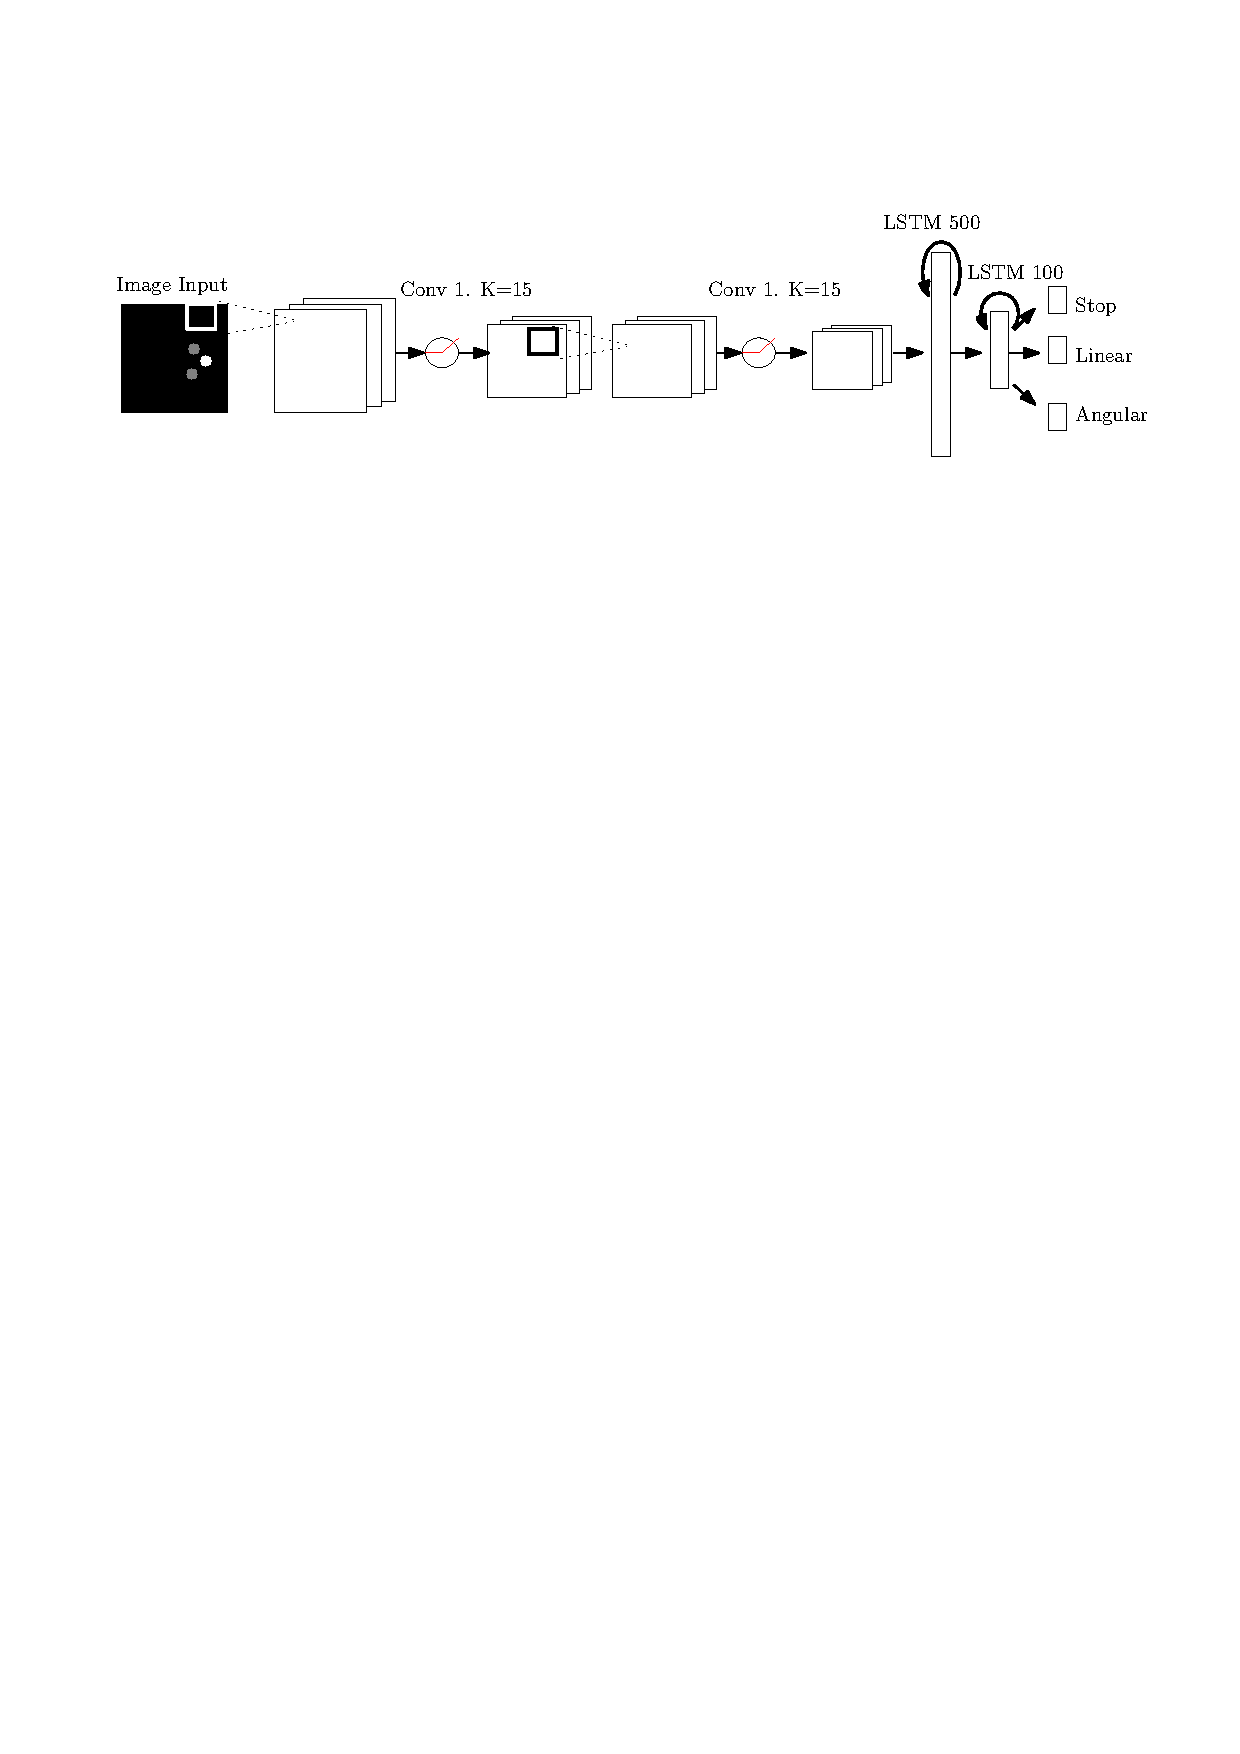
\includegraphics[width=0.9\textwidth]{figures/net.pdf}
	%\vspace{-4mm}
	  \caption[DNN Architecture]{The DNN architecture used to learn body pose policies from demonstration.}
	  \label{fig:pipeline}
	\end{figure}

\subsubsection{Continuous Learning Pipeline}
	In addition to the original experiments, we have created a learning pipeline for the robot that allows any human teacher to simply enrich the data that the networks is learned with. The pipeline runs as follows. First the most recently learned policy is deployed on the robot. The robot is then used for several interactions. During these interactions the robot is autonomous, however if any bad behaviour occurs the human demonstrator intervenes giving commands through a joystick. Any human intervention is then recorded by the robot. At the end of the interaction session any collected demonstrations are processed automatically and added to the rest of the data. Overnight the robot used the whole dataset to learn a new policy, at which point the process can be repeated. An outline of our learning pipeline is shown in Figure \ref{fig:pipeline}
	
	
	\begin{figure}
	\centering
	%\vspace{-3.3mm}
	    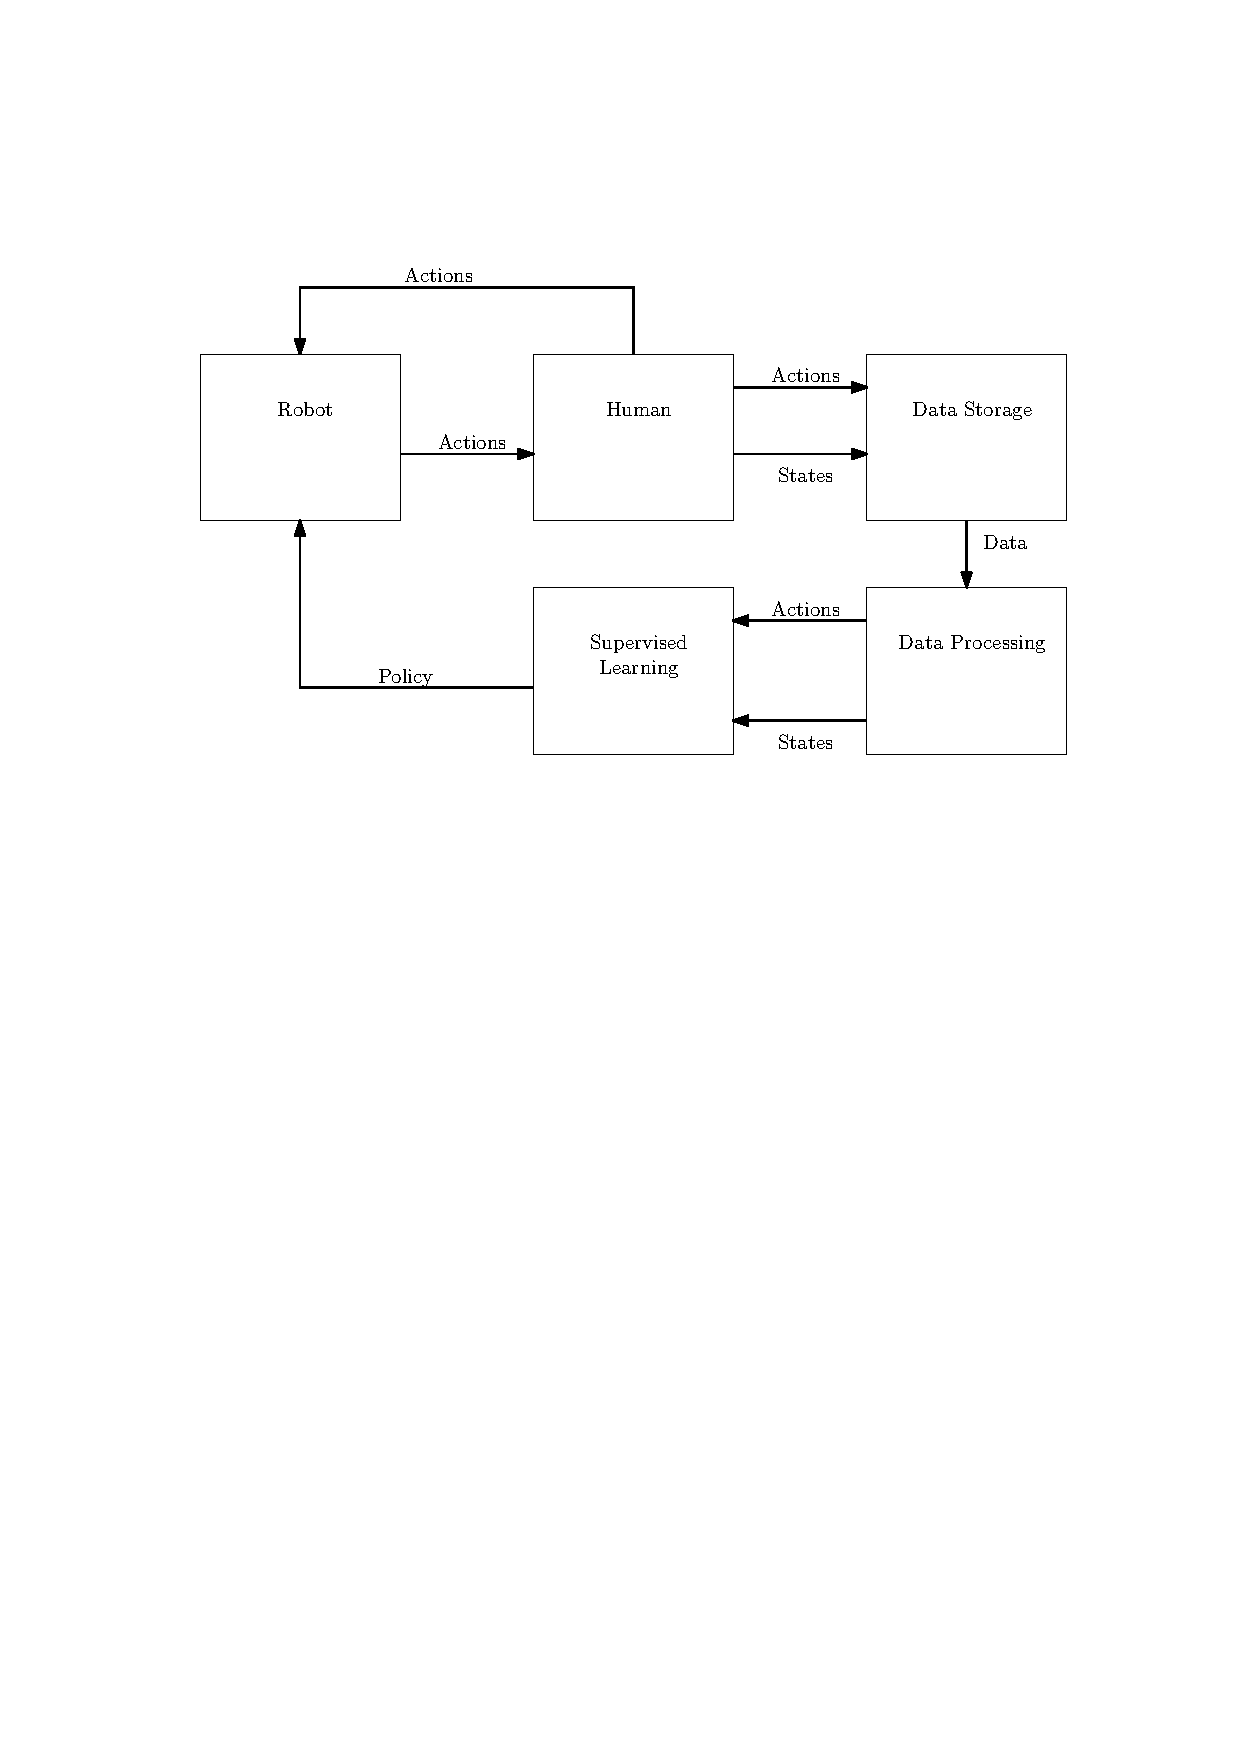
\includegraphics[width=0.8\textwidth]{figures/pipeline.pdf}
	%\vspace{-4mm}
	  \caption[Pipeline]{The continuous learning pipeline.}
	  \label{fig:pipeline}
	\end{figure}


\subsection{Results}\label{sec:sl_res}
In this section we plot the learning performance in terms of train and test loss for 3 output architectures. These are shown in Figures \ref{fig:SL_results}. Both discrete architectures have an action space of $v=\omega = [-0.5,-0.4,-0.3,0,0.3,0.4,0.5]$ hence each output has 7 classes. In the hierarchical case we have another binary output representing wether the robot should move or not. Because of this extra loss the two discrete architecture metrics are not comparable.

 I will perform a standardised comparison in terms of the hierarchical-non-hierarchical cases soon.

\begin{figure}[t]
	\centering
%	\hspace{-5cm}
      \begin{subfigure}[b]{0.45\columnwidth}

    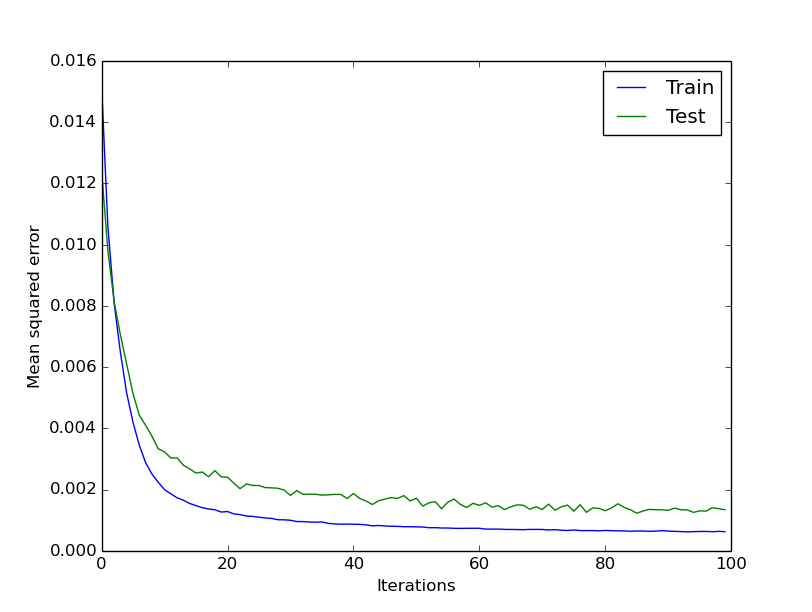
\includegraphics[clip=true,width=1.\textwidth]{figures/mse.png}
    \caption{Continuous}
    \label{fig:cont_results}
  \end{subfigure}
 % \hspace{5mm}
  \begin{subfigure}[b]{0.45\columnwidth}
    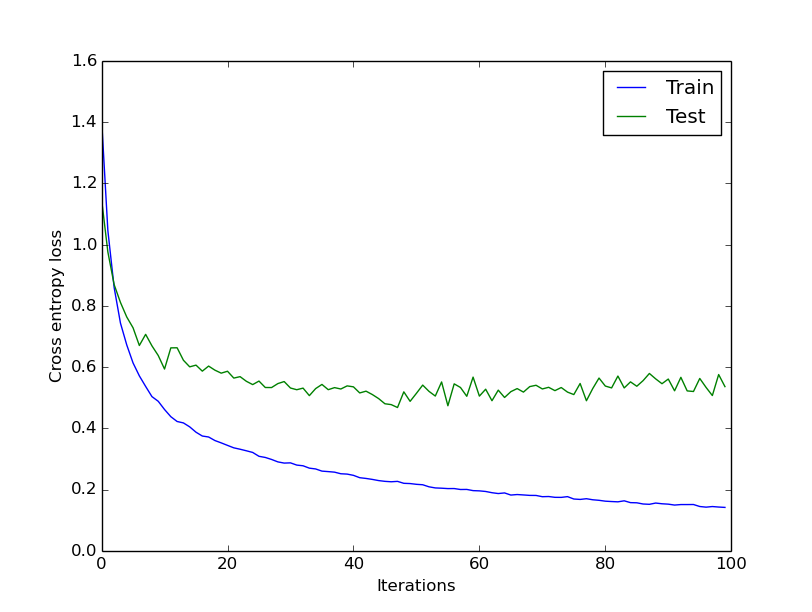
\includegraphics[clip=true,width=1.\textwidth]{figures/d_xent.png}
    \caption{Discrete}
    \label{fig:discrete_results}
  \end{subfigure} 
  
    \begin{subfigure}[b]{0.45\columnwidth}
    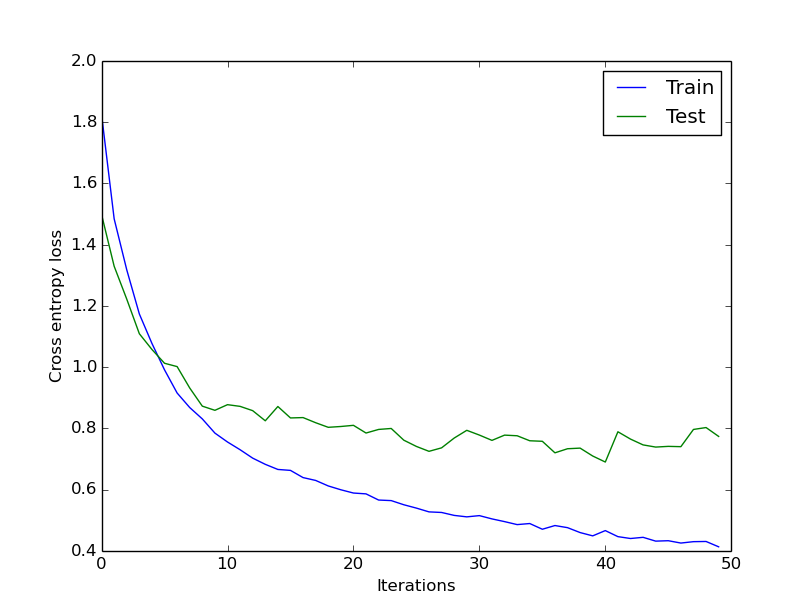
\includegraphics[clip=true,width=1.\textwidth]{figures/dh_xent.png}
    \caption{Hierarchical and discrete}
    \label{fig:hier_discrete_results}
  \end{subfigure} 

  %\vspace{-3mm}
  \caption[SL train test]{Train and test loss for the supervised learning under different output representations}
  %\vspace{-3mm}
  \label{fig:SL_results}
\end{figure}

Empirical results from the deployment of these policies can be found in Deliverable 5.4. 

\clearpage


\section{Integrating cost functions and human demonstrations (WIP)} \label{sl+rl}
\subsection{Introduction}
In the previous section we employed a DNN architecture to learn a social body pose policy from demonstrations, which is this section we refer to as the SL policy. One might argue however, that this would require a lot of samples from human demonstrations in order to result in a satisfactory behaviour for the robot. In this case Reinforcement Learining (RL) could be a more viable option for learning policies. In RL, one only needs to encode the preferences of a user in a cost(or reward) function and using that the robot can learn continuously. Designing a social cost function for our purposes however can be very challenging. One way to combat this drawback would be to use Inverse Reinforcement Learning (IRL) along with the collected human demonstrations. IRL was discussed in this and previous deliverables and has played a key role in deriving our navigation cost functions. The problem in this case is that our domain is partially observable and high dimentional. This means that we would need to use model free IRL methods such as [CITE REIRL] which can be very time consuming and still unreliable. In this section we take a slightly different approach. We investigate the possibility of using the policy learned from human demonstrations in combination with a hand coded cost function with the aim of learning a policy that both mimics the demonstrations and minimises the required cost simultaneously and prefferebly without any tradeoff. By doing so we aim to:

\begin{itemize}
	\item Use the policy from human demonstrations to learn faster using RL.
	\item Using RL to improve the SL policy where we feel is not peforming adequetly.   
\end{itemize}

In this section we propose a method that can integrate SL policies with hand coded cost(reward) functions and we show that for reasonable cost functions the above requirements can be satisfied. We begin with an introduction to basic policy gradient mathods for reinforcement learning in Section \ref{sec:pg_background}. We proceed to propose a simple cost function that tests our requirements above as well as an exploration strategy for the RL algorithm, this is done in Section ??. Finally we present some results in Section ?? and discuss future work in Section ??.


\subsection{Background}\label{sec:pg_background}

We assume a Markov decision process (MDP) with a state space $\mathcal{S}$ and an action space $\mathcal{A}$ an agent takes an action $a$ at a state $s$ according to a policy $\pi_\theta(s,a)$ where $\theta$ are the parameters of the policy, in our case the parameters of the neural network. For each state action pair the environment returns a reward $r(s,a)$ and the agent transitions to a next state according to a stationary dynamics dystribution $p(s_{t+1}|s_t,a_t)$. A sample return $r^{\gamma}$ is the discounted sum of rewards according to a discount factor $\gamma$. The Value function for a policy is defined as the expected return that results from following a policy $\pi$ starting at state $s$,


\begin{equation}
	V^{\pi}(s) = \mathbb{E}[r^{\gamma}|\pi,s]
\end{equation}

and the Action-Value function is defined as the expected return that results from starting at state $s$, taking action $a$ and then following policy $\pi$

\begin{equation}
	Q^{\pi}(s,a) = \mathbb{E}[r^{\gamma}|\pi,s,a]
\end{equation}


The traditional methods for learning in RL are based upon an agent learning $Q(s,a)$. Once this quantity is learned for all states and actions an agent can act greedily with respect to this function meaning that the action $a$ at state $s$ will be taken according to:
\begin{equation}
	a = \argmax_a Q(s,a) \label{eq:Q}
\end{equation}

Because the maximisation in \ref{eq:Q} can sometimes be very hard to perform, e.g in continuous spaces, policy gradient [cite barto] methods usually act as an alternative. In this section we do not consider a continuous action space for the sake of simplicity, we do however use policy gradient methods. This is because we aim to integrade our SL policy with cost functions. Since our DNN already outputs actions and not $Q(s,a)$ it is much more straighforward to make this integration happen using policy gradient methods. In this work we use the REINFORCE algorithm \cite{williams1992simple} which we review here. 

A policy search methods attempt to optimise a performance objective defined as:

\begin{equation}
	J(\pi_{\theta}) = \int_{\mathcal{S}} \rho(s)^{\pi} \int_{\mathcal{A}}\pi_{\theta}(s,a)r(s,a)dads
\end{equation}

Where, $ \rho(s)^{\pi}$ is the state visitation distribution under policy $\pi$ and the current dynamics.
Policy gradient methods attempt to perform gradient descent on this objective. The policy gradient theorem [cite barto] states that the gradient of the objective with respect to the policy parameters $\theta$ does not depend of the state distribution.

\begin{align}
	\nabla_{\theta}J(\pi_{\theta}) &= \int_{\mathcal{S}} \rho(s)^{\pi} \int_{\mathcal{A}}\nabla_{\theta}\pi_{\theta}(s,a)Q^{\pi}(s,a)dads\\
	&= \mathbb{E}_{\rho^{\pi},\pi_{\theta}} [\nabla_{\theta}\log\pi_{\theta}(s,a)Q^{\pi}(s,a)]
\end{align}

The REINFORCE algrotithm calculates $Q^{\pi}(s,a)$ using discounted sample returns.
In the case of our SL policy derived in the previous section, it could be the case that although the output is stochastic the network is too confident about a certain action. This would prevent any exploration from the agent which would make learning slow and possibly inneffective. In this case it is useful to act according to a different behaviour policy $\beta(s,a)$ while computing a gradient for our original policy $pi_{\theta}(s,a)$. The only modification to equation ?? would be weighing the gradient by an importance ratio, i.e.,  

\begin{equation}
\nabla_{\theta}J(\pi_{\theta}) = \mathbb{E}_{\rho^{\beta},\beta_{\theta}} [\frac{\pi_{\theta}(s,a)}{\beta_{\theta}(s,a)}\nabla_{\theta}\log\pi_{\theta}(s,a)Q^{\pi}(s,a)]
\end{equation}




\subsection{Implementation}
In this section we describe the aspects of the algorithm specific to out implementation of REINFORCE. The state representation remains the one we have described in Section \ref{sec:demonstration_experiment}. As an action representation we use a non-hierachical discretised action representation.

\subsubsection{Learning scenario and reward function}

As a proof of concept we use a simulated static scenario where two persons are standing in the middle of a square room as shown in Figure ??. The robot is spawned at different orientations and positions around the persons every 40 seconds, which we consider the duration of one episode. Although there are two persons in the scene, only one of the two is considered the interaction target. Hence in our image input representation only one circle is given a value of 2 and the other a value of 1. The reward function in this scenario consists of two parts. The first which we name $r_i$ is a based on the orientation of the robot with respect to the interaction target. 

\begin{equation}
	r_i = \frac{\pi}{3} -|\phi_{rel}| 
\end{equation}

The second part is a reward based on the distance of the robot to each person (Figure \ref{fig:rd}). We penalise the robot being either too close or too far away from the people in the room. To do so, for each person we consider the distance based reward for person $p$, $r_{d_p}$ to be the addition of two sigmoids.

\begin{equation}
	r_{d_p} = \frac{-2}{1+\exp(22-10x)}+ \frac{-2}{1+\exp(-7+10x)} 
\end{equation}
where x is the eucledian distance from the robot.

	\begin{figure}
	\centering
	%\vspace{-3.3mm}
	    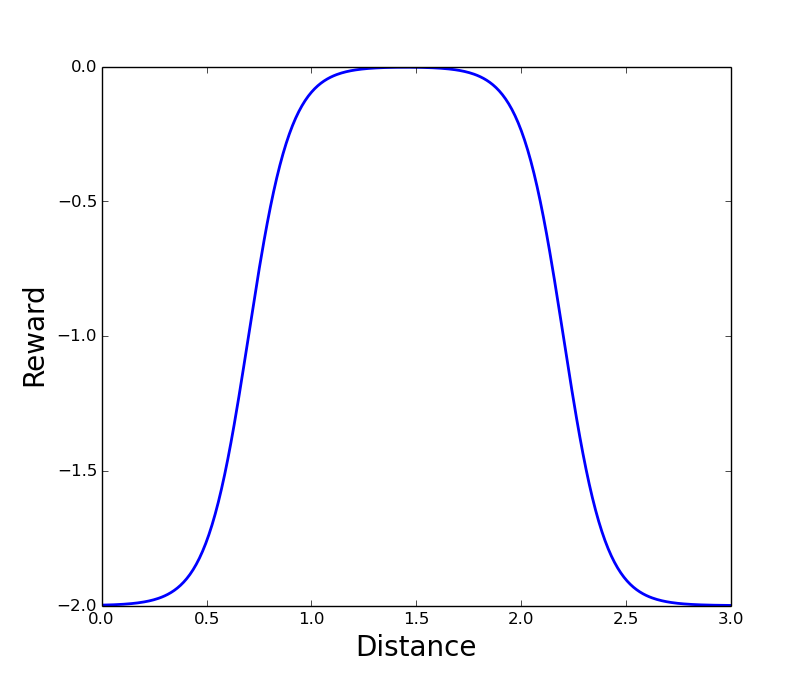
\includegraphics[width=0.5\textwidth]{figures/rd.png}
	%\vspace{-4mm}
	  \caption[Distance based reward function]{Reward function based on the distance of the robot from the simulated people in the scene.}
	  \label{fig:rd}
	\end{figure}
	
The total reward is given as the addition of $r_i$ and the two $r_{d_p}$ reward functions (one for each person in the scene). Figure \ref{fig:int_reward} depicts an example of the reward function for various positions of the interaction target.
 
 	\begin{figure}
	\centering
	%\vspace{-3.3mm}
	    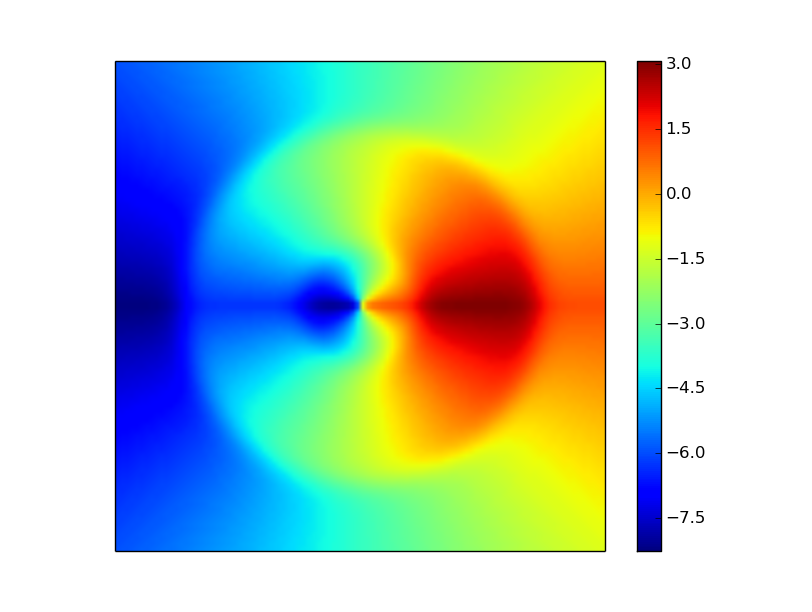
\includegraphics[width=0.5\textwidth]{figures/int_reward.png}
	%\vspace{-4mm}
	  \caption[Interaction target reward]{Reward function for the interaction target.}
	  \label{fig:int_reward}
	\end{figure}

\subsubsection{Exploration}
In order to promote our pre-trained SL policy to explore different actions exploration policies can be used. One very basic form of exploration policy is $\epsilon-$greedy. Under this exploration policy the agent takes the action prescribed by the policy with probability $1-\epsilon$ and with probability $\epsilon$ takes a unoformly random action from $A$. This is fine for most applications, however for control applications like ours the control rate of the agent is quite high (10Hz) and actions that are similar in magnitute have similar dynamics assosciated with them. This means that it makes more sense for the agent to explore actions around the previous action rather than picking an action at random. In recent work researchers use different forms of correlated processes in order to generate useful exploratory trajectories, for example in \cite{lillicrap2015continuous} the authors use an  Ornstein-Uhlenbeck process \cite{uhlenbeck1930theory}. In our case we do not have continuous actions and thus take a slightly different approach to produce correlated action samples. 

Supose we have 7 available actions to choose from. Instead of choosin an action with uniform probability we place a Gaussian function with a mean on the previous action \emph{index} $a^{idx}_{t-1}$ and a scale c. We can then calculate the probability of action index at time $t$, $a^{idx}_{t-1}$ according to,   


\begin{equation}
	p(a^{idx}_t) =\frac{\exp(-\frac{(a^{idx}_t-a^{idx}_{t-1})^2}{2c^2})}{\sum_i^{|\mathcal{A}|} \exp(-\frac{(a^{idx}_i-a^{idx}_{t-1})^2}{2c^2}) }.
\end{equation}

Figure ?? plots the distance based reward for a single person as a function of the eucledian distance x from the robot. 



This means that we give a greater weight for actions closer in index to our previous action and assuming that actions closer in index are more similar as in our case we can achieve a correlated noise effect. A sample of such an action process is shown in Figure for various values of the scale $c$. We can see that a when $c=1.1$ the action sequence is much more reasonable for any physical system than the case where $c=20$, which is essentially like drawing samples from a uniform distribution. 


\begin{figure}[t]
	\centering
%	\hspace{-5cm}
      \begin{subfigure}[b]{0.45\columnwidth}

    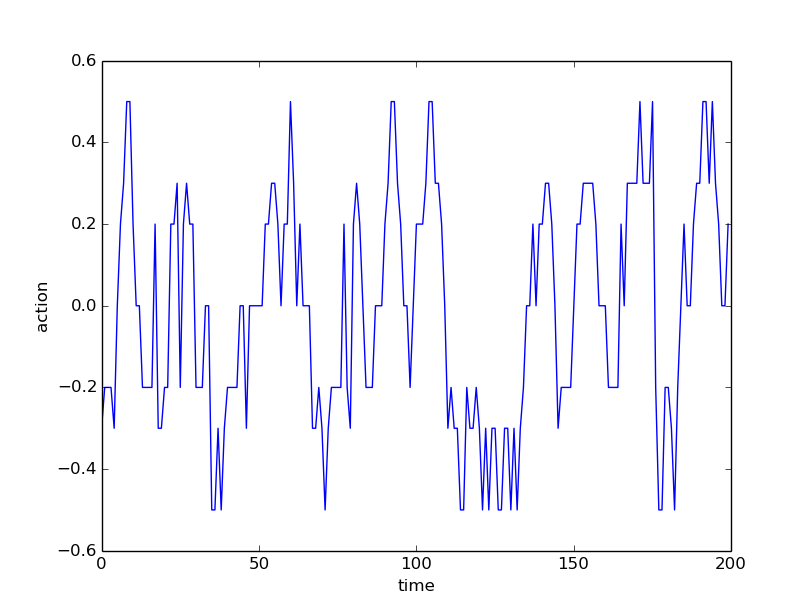
\includegraphics[clip=true,width=1.\textwidth]{figures/action_11.png}
    \caption{c = 1.1}
    \label{fig:c_11}
  \end{subfigure}
 % \hspace{5mm}
  \begin{subfigure}[b]{0.45\columnwidth}
    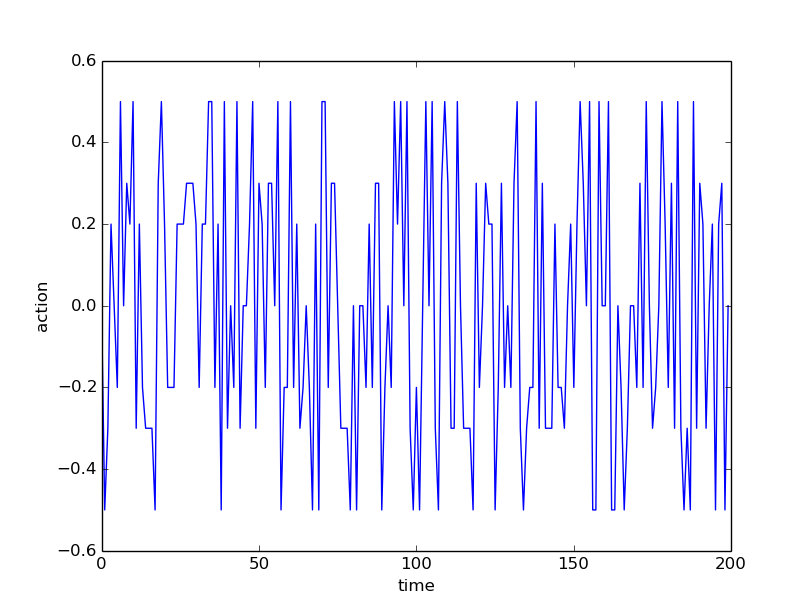
\includegraphics[clip=true,width=1.\textwidth]{figures/action_c20.png}
    \caption{c=20}
    \label{fig:c_20}
  \end{subfigure} 

  %\vspace{-3mm}
  \caption[Exploration at different parameters]{Exploration at different values of the Gaussian scale parameter, $c$.}
  %\vspace{-3mm}
  \label{fig:exploration}
\end{figure}

\subsection{Results}
In this section our aim was to show that by using policy gradient RL methods we can learn a policy that can perform well both in terms of the initial SL policy and the specified reward function. We further claimed that if the reward function was reasonably close to the human prefereces in the demonstrations it will also allow the RL algorithm to learn better. In this section we document out results with respect to these aims. Our method named RL+SL is compated to cases where only one learning paradigm is used. The method named $RL_{only}$ uses reinforcement learning on the reward function above, while the method $SL_{only}$ only learns a policy using the demonstrations as in the previous section. We perform a comparison of these 3 methods both in terms of the cost function described above and in terms of the human demonstrations.

\subsection{Comparison with RL}
In this first comparison we use our SL policy as a starting point and then use the cost function described above to learn a new policy using RL. We compare this to learning using RL from scratch, i.e starting with a random policy and with usign the SL policy without any learning. Figure ?? plots the average reward over 10000 timesteps for each method. Figure ?? shows the histograms of rewards for batches of 10000 timesteps for each algorithm. We can see that there is a clear advantage to using SL+RL than any of the two methods on their own. This advantage comes both in terms of speed of learning as well as the convereged policy.

\subsection{Comparison with SL}
After using RL on the three policies we can go back and see how they perform on the supervised data. This can be done by simply measuring the total cross entropy loss for the whole demonstration dataset collected, without performing any learning. The results are summarised in Table ??, we can clearly see that...  

\section{Integrating different cost functions using a multi-objective approach}
For the TERESA project, we have different sources of reward/cost (Section \ref{sec:integratecost}). When there are multiple sources of possibly conflicting feedback with respect to the socially optimal behaviour of the telepresence robot, e.g.,  corresponding to the user experience of the pilot (i.e., the person who steers the robot from a distance) and to the user experience of the target(s) (the person(s) with whom the robot is collocated and interacts directly), it is unclear what the best way is to integrate these. In the previous section, we have integrated different sources of cost manually, a priori. However, a theoretically more grounded way would be to see the different sources of cost as different objectives, and compute a set of policies for the robot that make different trade-offs between these objectives. This leads to so-called multi-objective decision making. 

We explored the possibilities for using multi-objective decision making \cite{roijers13survey, roijersPhD} for social robotics,  where different sources of feedback correspond to multiple objectives that we would like to optimise simultaneously. However, because these objectives may be conflicting, there is typically no single policy that attains the optimal value for each objective. Therefore, we must compute a so-called coverage set (CS) \cite{roijers13survey}, that contains at least one optimal policy for each possible utility function (i.e., preference) that a user might have with respect to the objectives. Because different users might have different interests while interacting with the robot, we take the utility function of the robot designer as the ultimate goal. We assume that this utility function is unobservable at the time when we need to plan different policies, and can only be partially observed after different policies have been computed, as a result of expressed preferences between different alternative policies.

In order to model different sources of feedback, we make use of an extension to the partially observable Markov decision process (POMDP) model \cite{Kaelbling98} that we have used in this and earlier work packages. Specifically, in a multi-objective partially observable Markov decision process (MOPOMDP) \cite{soh2011,roijers2015point,wray2015} the states, actions, transition function, observations and observation function are the same as in a POMDP, but the reward function is vector-valued, i.e., each element of the reward vector corresponding to a transition, corresponds to a different objective. 

In the following subsections we investigate the following questions: 1) which different sources of feedback can be obtain reliable data for, and how can we translate these different sources of feedback into a MOPOMDP; 2) what is an appropriate coverage set for this MOPOMDP and how can we compute it; and 3) how can we perform user selection in an effective way such that the robot designer can make an informed decision about which policy to select and ultimately implement in the robot. Finally, we discuss why this approach did not work well in this setting (yet), and promising alleys for further investigation for multiple objectives for robotics, such as deep multi-objective reinforcement learning (which would mitigate the need for using an explicit MOPOMDP model). 

\subsection{Sources of feedback}
In order to present policies that account for different objectives, we must first consider which sources of feedback we can obtain. In our original plan, we planned to have two objectives corresponding to the pilot resp. the target(s). In this setting, we would gather data from the interaction targets as well as the pilot in the following way: each person would observe robot behaviour in real-life experiments, and press a negative feedback button when the robot behaved badly. This would result in two objectives, corresponding to different roles. When gathering this data, it would be vitally important to see a difference between different behaviours in a) what is bad and what is not, but also b) which behaviours are worse than other bad behaviours. Sadly, we were unable to collect data to show this sufficiently. Therefore, we decided to focus on pilot feedback only. 

The pilot had two interests while controlling the robot. Firstly, the behaviour of the robot must be socially acceptable. This can be expressed by giving explicit feedback. However, for the pilot to be able to use the system adequately, the robot must also detect people accurately enough (so that the pilot can select different interaction targets). We thus aimed to obtain data corresponding to three objectives: negative feedback on the social behaviour of the robot (inputted by the pilot) to minimise, and false positive detections and false negative detections (to be determined experimentally). 

In order to gather this data, we used the single-interaction target approach scenario with no other people in the room. We used the wizard-of-oz approach, where the experimenter would control the robot. The wizard would show both behaviour that she would find socially acceptable, and socially unacceptable behaviour, while approaching the target. The pilot would speak with the interaction target over the robot, while giving negative feedback if the robot behaved badly. 

When we tested this, we found that in this setting we would not have any false positives in the gathered data, and were therefore limited to two objectives: minimising the expected negative feedback from the pilot, while minimising the number of false negative detections (i.e., failures to detect the interaction target). We not however, that the feedback from the pilot was rather sparse, as indicated in the next section. 

\subsection{MOPOMDP modelling}

In this section we describe the standard MOPOMDP formulation. We have one interaction target, and no other people in the scenario. Therefore we define the state with this interaction target as the origin. The state consists of an angle and a distance with respect to the interaction target. Both these components are discretised. 


The social reward function for the interaction target is learned from data, from feedback from the pilot of the robot, and is state-based. However, the data to learn this social reward function was sparse, the learned function may be estimated wrongly. We aim to improve the previously learned social reward function by imposing extra constraints on e.g., the smoothness of the social reward function. The detection reward are defined as the number of time steps where a false negative detection takes place.  The detection reward must also be learned from data.

The resulting multi-objective POMDP is  a tuple $\langle S,A,R,T,\Omega,O,\gamma\rangle$ where 
\begin{itemize}
\item $S = < S_{\varphi}, S_{d}>$ is the state space consisting of an angle ($S_{\varphi}$) and a distance  ($S_{d}$) component. 
\begin{itemize}
\item $S_{d} = \{\mathtt{far}, \mathtt{opt_{detect}}, \dots, \mathtt{to}_i, \dots, \mathtt{opt_{social}}, \mathtt{close}\}$ where, 
\item $\mathtt{far}$ is too far away
\item $\mathtt{close}$ is too close
\item $\mathtt{opt_{detect}}$ is the optimal detection distance (interval)
\item $\mathtt{opt_{social}}$ is the optimal detection distance (interval)
\item $\mathtt{to}_i$ are $N_{to}$ equally space trade-off intervals, where $N_{to}$ is minimally $1$ and maximally $5$. 
\item $S_{\varphi}$ is a set of angle intervals, dividing the angles in equal parts within the field of vision (45 degrees to the left or right w.r.t. straight in front), and one behind. $N_{\varphi}$ is the number of intervals. $N_{\varphi}$ needs to be even.
\end{itemize}
\item $A = \{\mathtt{wait}, \mathtt{forward}, \mathtt{backward}, \mathtt{turnleft}, \mathtt{turnright}\}$ is the (self-explanatory) action space.
\item ${\bf R}(s,a,s') = {\bf R}(s')  = ({R}_{soc}(s'), {R}_{fp}(s'))$ is the 2-objective reward function consisting of the state-based social reward, and the (also state-based) detection reward.  The reward depends on the discretisation of the state, and must thus be relearned every time we adjust $N_{to}$ and $N_{\varphi}$.
\begin{itemize}
\item ${R}_{soc}(s')$ is negative and learned from the negative feedback pilots gave explicitly in earlier experiments. To make this function more usable than we currently have we need to learn this function with smoothness constraints. ${R}_{soc}(s')$ only depends on the distance feature of the state space: $S_{d}$. 

\item ${R}_{fn}(s')$ is the number of false negative detections based on the result state after taking an action. This depends on both the angle and the distance, i.e., the full state $S$. 
\end{itemize}
\item $T(s,a,s')$ is the transition function, giving the probability of a next state given an action and a current state; needs to be learned from data. 
\item $\Omega = < \Omega_{d}, \Omega_{\varphi} >$ is the set of observations, equal in size to $S$. 

\item $O$ is the observation function, giving the probability of each observation given an action and the resulting state. One special remark here is that the observation probability is equal to the detection probability used for the reward function. We note that the detection is done by a separate module, i.e., putting circles around people is ``outsourced''. A function exists that estimates the probability of accurate detection, but that is currently not over the same state-space. We thus have to re-learn this. 
\item $\gamma$ is the discount factor. 
\end{itemize}

As in previous sections, we learn the transition, reward and observation functions using the wizard-of-oz approach, by counting the transitions from each state to each state, the social feedback given in each state, the number of false negatives in each state, and the observations for each state-action pair. 

\subsection{Solution and algorithms}
We assume that the utility function of the user can be seen as a linear combination of the value of a policy in each objective. However, we must take into account that this assumption might be an oversimplification. 

In the planning phase, we can thus assume that the value of a policy can be linearly scalarised, but we do not know the correct weights. Therefore, in the planning phase we must aim to compute a convex coverage set, i.e., the a set of policies that contains at least one optimal policy for each (linear) weighting of the objectives.  When all weight is given to the social feedback objective, the robot will just aim to minimise this feedback signal. When some weight is given to the second objective, the agent will be more likely to perform actions that provide correct detections to the pilot of the system.  
We can compute a convex coverage set for an MOPOMDP, using the state-of-the-art optimistic linear support with alpha reuse (OLSAR) planning algorithm \cite{roijers2015point} (out of the box).  

\subsection{Evaluation}\label{sec:evalMO}
After computing the convex coverage set, we show different policies to the users of the system. However, we cannot simply show the policy values with respect to social feedback and detection errors, and expect the user to be able to interpret these values. Instead, we ran the policies in a simulator, and plotted: a) the trajectory of the robot, and b) the detections it made. Such a plot took about 30 minutes to plot, using the Gazeebo simulator on ROS. In this way, we hoped that the policies would be able to be comparable in a meaningful way to the user. 

However, we ran into several problems that we could not overcome: 
\begin{itemize}
\item The trajectories resulting from our planner look like Figure \ref{fig:motraj}. These trajectories appear jittery. In fact, it is hard to distinguish any differences between trajectories learned for different linear scalarisation weights. 
\item Aggravating this situation is that the objectives where highly correlated. Therefore, even if the agent would know where it was perfectly, the robot would take the same actions in most of the state-space. I.e., in large parts of the state-space, the policies also \emph{need to be} indistinguishable. 
end{itemize}
Therefore, we conclude that --- while we still believe multiple objectives could contribute to social robotics --- for this use case, a user could not meaningfully select a policy from the convex coverage set. 
\begin{figure}
\centering
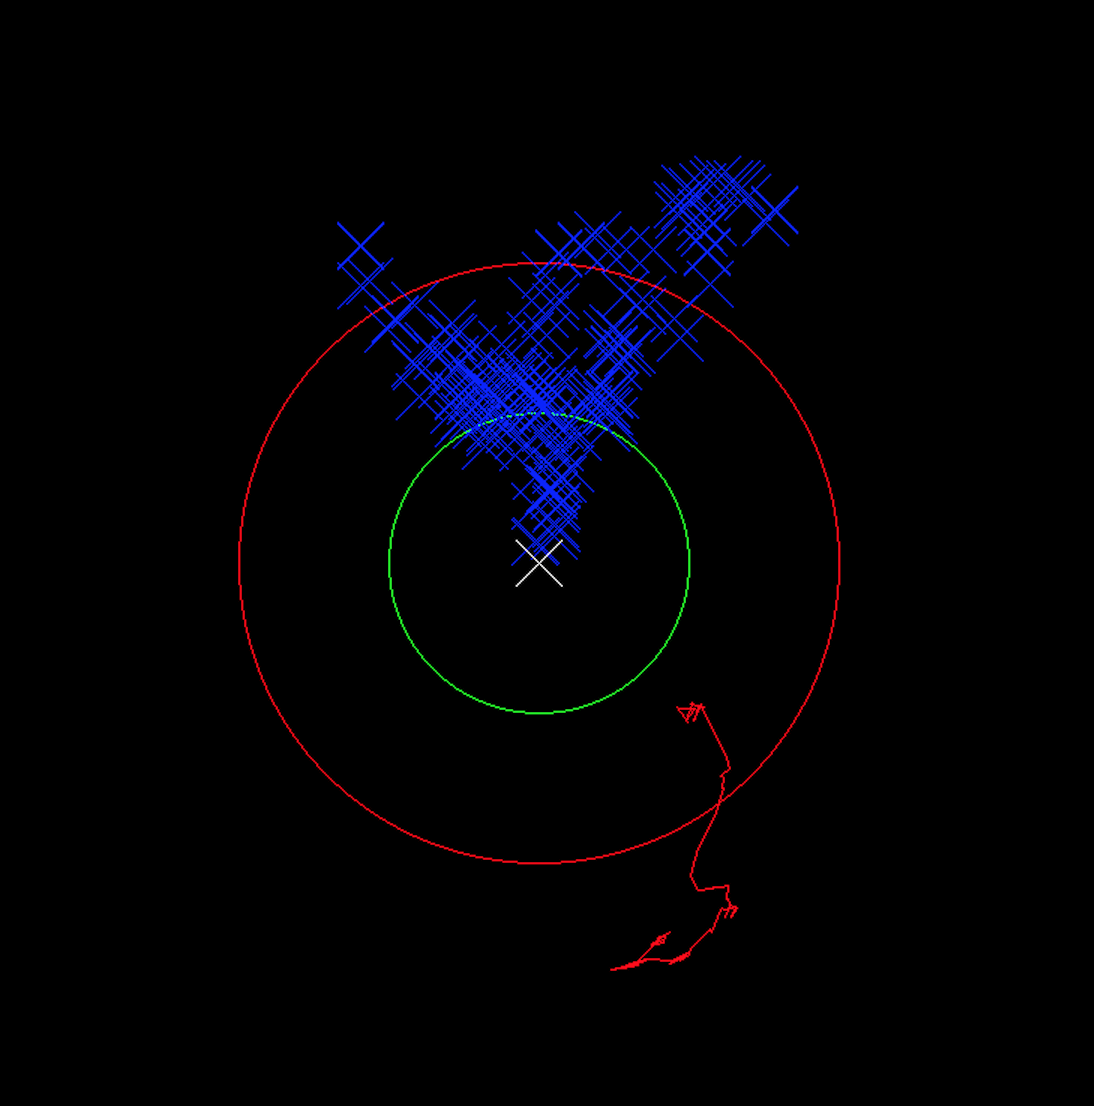
\includegraphics[width=0.4\textwidth]{motrajectory.png}
\caption[Robot interaction trajectory]{A trajectory of the social robot (in red) interacting with a target (the gray 
cross), making detections (the blue crosses), and finding a balance between the optimal 
detection distance (the red circle) and the optimal social distance (the green circle).}
\label{fig:motraj}
\end{figure}
\end{itemize}

\subsection{Lessons learnt and future research directions}
While trying to model a social robotics problem as a multi-objective decision problem we ran into a several problems (see Section \ref{sec:evalMO}). From these, we draw the following conclusion: when the objectives are highly correlated, a lot of data is needed in order to create a MOPOMDP model that can lead to policies that make distinguishably different trade-offs between the objectives. Hence, when little data is available, multi-objective approaches with highly conflicting objectives could be promising for modelling as a MOPOMDP.  Having set this, we believe that multi-objective methods can be vital for solving decision problems in social robotics. Particularly, we think the following cases should be investigated taking a multi-objective approach: 
\begin{itemize}
\item Extending existing robotics tasks that have a clearly described reward such as cleaning or path planning, to a setting in which it social costs resulting from the presence of humans. In such cases, minimising the social costs will typically be conflicting with maximising the efficiency with which the task is performed, e.g., robotics may have to take a longer route to not disturb the humans. However, in some cases it may be acceptable to cause some hindrance to humans by taking a shorter path that avoids humans to some extent. In fact, that is what humans do themselves as well. 
\item Social robotics tasks in which the social costs for different (groups of) users are clearly conflicting. For example, consider a group of people walking together with a telepresence robot, and a different group of people crossing the first group's path. If the robot would be overly considerate of the latter group, this may hinder the conversation in the former group. 
\end{itemize}

\subsubsection{Multi-objective deep reinforcement learning}
Furthermore, we also believe that it would be highly promising to use techniques that do not require modelling an entire MOPOMDP. For single-objective settings, we have already mentioned LSTMs and RNNs. The power of these models is that they can generalise over states automatically, without designer intervention. However, in order to train these neural networks from interaction data, multi-objective deep reinforcement learning methods needed to be developed. 

We developed the to our knowledge first deep multi-objective reinforcement learning algorithm, called Deep Optimistic Linear Support Learning (DOL) \cite{hossam2016}. DOL is built on Deep Q-Learning with standard (non-recurrent) deep Q-networks, and has so far been shown to work on problems that do not have the additional challenges of a) having to be learnt from physical interactions with a robot, and b) are not partially observable. In future work, we aim to create methods for deep multi-objective reinforcement learning, that can handle partially observable states (as is typically the case in social robotics settings) by incorporating memory (via LSTMs or RNNs), and apply these to our telepresence robot. In order to make such methods work for our telepresence robot, special attention must be paid to sample efficiency, as the sessions for gathering data with the telepresence robot are a scarce resource. 

\section{Conclusions and Future Work in Tasks 5.1 and 5.2}
\label{sec:conclusions}
This deliverable has summarised our progress for Work Package 5 from month 15 of the project until month 30. Significant progress has been achieved in all aspects of social behaviour learning on the TERESA robot. 

 An important aspect of this progress is in terms of learning from human demonstrations, using IRL. Firstly we have enabled the robot to learn from failed demosntrations as well as succesful ones in a unified principled framework. We have demonstrated that our method is capable of utilising the failed demonstrations in conjunction with the succesful ones to learn faster and better. Secondly we have developed a novel IRL method called, RLT$^*$ that works with RRT$^*$ as the underlying planner. RRT's are at the heart of TERESA's path planning module, thus learning directly using this planners is bound to produce superior learning results. We have also shown that our method is faster and better that a similar method that uses deterministic planners. A clear avenue of future work is to deploy RLT$^*$ on the real system. Furthermore we plan to integrate these methods together and evaluate any improvement on the real system.

 We have also reported significant progress in terms of experimentation and implementation of social conversation policies. Specifically, we conducted experiments and performed the necessary analysis, in order to discover a cost function for the distance between the robot and the interaction target. In addition we performed statistical analysis on an existing dataset gathered by our partners at UT. This dataset consisted of groups of people scoring how well the TERESA robot approached them. This analysis allowed us to produce a second cost function that determines how the robot should be orientated in such situations. The analysis also concluded that the bearing of the robot to the group's geometric centre was far more important to the bearing with respect to an individual person. This allowed us to determine a compact yet representative state-space representation for the robot during conversation. 

In terms of social conversation, there are three directions of future work we are currently pursuing, and for which we plan to report in month 36. Firstly, we aim to apply the methods for IRL that were here presented to the problem of learning social cost functions for social conversation from expert demonstrations of the interaction behaviors; Secondly, we aim to integrate the available cost functions in order to learn a single social conversation policy under which the robot operates. Finally, we aim to make the resulting policy more robust to false positives from the robots social detectors using advanced filtering techniques such as \emph{partially observable Markov decision processes} (POMDPs) and \emph{long-short memory networks} (LSTMs).

\bibliographystyle{plain}
\bibliography{references.bib}

\end{document}
